% Options for packages loaded elsewhere
\PassOptionsToPackage{unicode}{hyperref}
\PassOptionsToPackage{hyphens}{url}
%
\documentclass[
]{book}
\usepackage{amsmath,amssymb}
\usepackage{iftex}
\ifPDFTeX
  \usepackage[T1]{fontenc}
  \usepackage[utf8]{inputenc}
  \usepackage{textcomp} % provide euro and other symbols
\else % if luatex or xetex
  \usepackage{unicode-math} % this also loads fontspec
  \defaultfontfeatures{Scale=MatchLowercase}
  \defaultfontfeatures[\rmfamily]{Ligatures=TeX,Scale=1}
\fi
\usepackage{lmodern}
\ifPDFTeX\else
  % xetex/luatex font selection
\fi
% Use upquote if available, for straight quotes in verbatim environments
\IfFileExists{upquote.sty}{\usepackage{upquote}}{}
\IfFileExists{microtype.sty}{% use microtype if available
  \usepackage[]{microtype}
  \UseMicrotypeSet[protrusion]{basicmath} % disable protrusion for tt fonts
}{}
\makeatletter
\@ifundefined{KOMAClassName}{% if non-KOMA class
  \IfFileExists{parskip.sty}{%
    \usepackage{parskip}
  }{% else
    \setlength{\parindent}{0pt}
    \setlength{\parskip}{6pt plus 2pt minus 1pt}}
}{% if KOMA class
  \KOMAoptions{parskip=half}}
\makeatother
\usepackage{xcolor}
\usepackage{longtable,booktabs,array}
\usepackage{calc} % for calculating minipage widths
% Correct order of tables after \paragraph or \subparagraph
\usepackage{etoolbox}
\makeatletter
\patchcmd\longtable{\par}{\if@noskipsec\mbox{}\fi\par}{}{}
\makeatother
% Allow footnotes in longtable head/foot
\IfFileExists{footnotehyper.sty}{\usepackage{footnotehyper}}{\usepackage{footnote}}
\makesavenoteenv{longtable}
\usepackage{graphicx}
\makeatletter
\def\maxwidth{\ifdim\Gin@nat@width>\linewidth\linewidth\else\Gin@nat@width\fi}
\def\maxheight{\ifdim\Gin@nat@height>\textheight\textheight\else\Gin@nat@height\fi}
\makeatother
% Scale images if necessary, so that they will not overflow the page
% margins by default, and it is still possible to overwrite the defaults
% using explicit options in \includegraphics[width, height, ...]{}
\setkeys{Gin}{width=\maxwidth,height=\maxheight,keepaspectratio}
% Set default figure placement to htbp
\makeatletter
\def\fps@figure{htbp}
\makeatother
\setlength{\emergencystretch}{3em} % prevent overfull lines
\providecommand{\tightlist}{%
  \setlength{\itemsep}{0pt}\setlength{\parskip}{0pt}}
\setcounter{secnumdepth}{5}
\usepackage{booktabs}
\usepackage{amsthm}
\makeatletter
\def\thm@space@setup{%
  \thm@preskip=8pt plus 2pt minus 4pt
  \thm@postskip=\thm@preskip
}
\makeatother
\ifLuaTeX
  \usepackage{selnolig}  % disable illegal ligatures
\fi
\usepackage[]{natbib}
\bibliographystyle{plainnat}
\IfFileExists{bookmark.sty}{\usepackage{bookmark}}{\usepackage{hyperref}}
\IfFileExists{xurl.sty}{\usepackage{xurl}}{} % add URL line breaks if available
\urlstyle{same}
\hypersetup{
  pdftitle={NCGR NISE-Bioinformatics},
  hidelinks,
  pdfcreator={LaTeX via pandoc}}

\title{NCGR NISE-Bioinformatics}
\author{}
\date{\vspace{-2.5em}}

\begin{document}
\maketitle

{
\setcounter{tocdepth}{1}
\tableofcontents
}
\hypertarget{national-center-for-genome-resources}{%
\chapter*{National Center for Genome Resources}\label{national-center-for-genome-resources}}
\addcontentsline{toc}{chapter}{National Center for Genome Resources}

This publication was supported by an Institutional Development Award (IDeA) from the National Institute of General Medical Sciences of the National Institutes of Health under grant number P20GM103451.

\hypertarget{license-and-copyright}{%
\section*{License and Copyright}\label{license-and-copyright}}
\addcontentsline{toc}{section}{License and Copyright}

Creative Commons Attribution-NonCommercial-NoDerivatives 4.0
\url{https://creativecommons.org/licenses/by-nc-nd/4.0/}

© 2023 National Center for Genome Resources

\hypertarget{linux}{%
\chapter{Linux}\label{linux}}

\textbf{Linux operating system (OS) and Bourne-Again SHell (bash) command-language basics}

\hypertarget{a-little-shell-aka-the-prompt-is-the-command-line-interface}{%
\section{A little shell\ldots{} aka the \$ prompt is the command line interface}\label{a-little-shell-aka-the-prompt-is-the-command-line-interface}}

\begin{itemize}
\tightlist
\item
  A shell is a user interface to the operating system.

  \begin{itemize}
  \tightlist
  \item
    CLI (Command Line Interface)
  \item
    GUI (Graphical User Interface)
  \end{itemize}
\item
  Bourne-Again SHell (bash) is a Unix shell and command language
\item
  Each command drives a program or script by talking to the Operating System
  (Linux)
\end{itemize}

\hypertarget{directory-structure}{%
\section{Directory Structure}\label{directory-structure}}

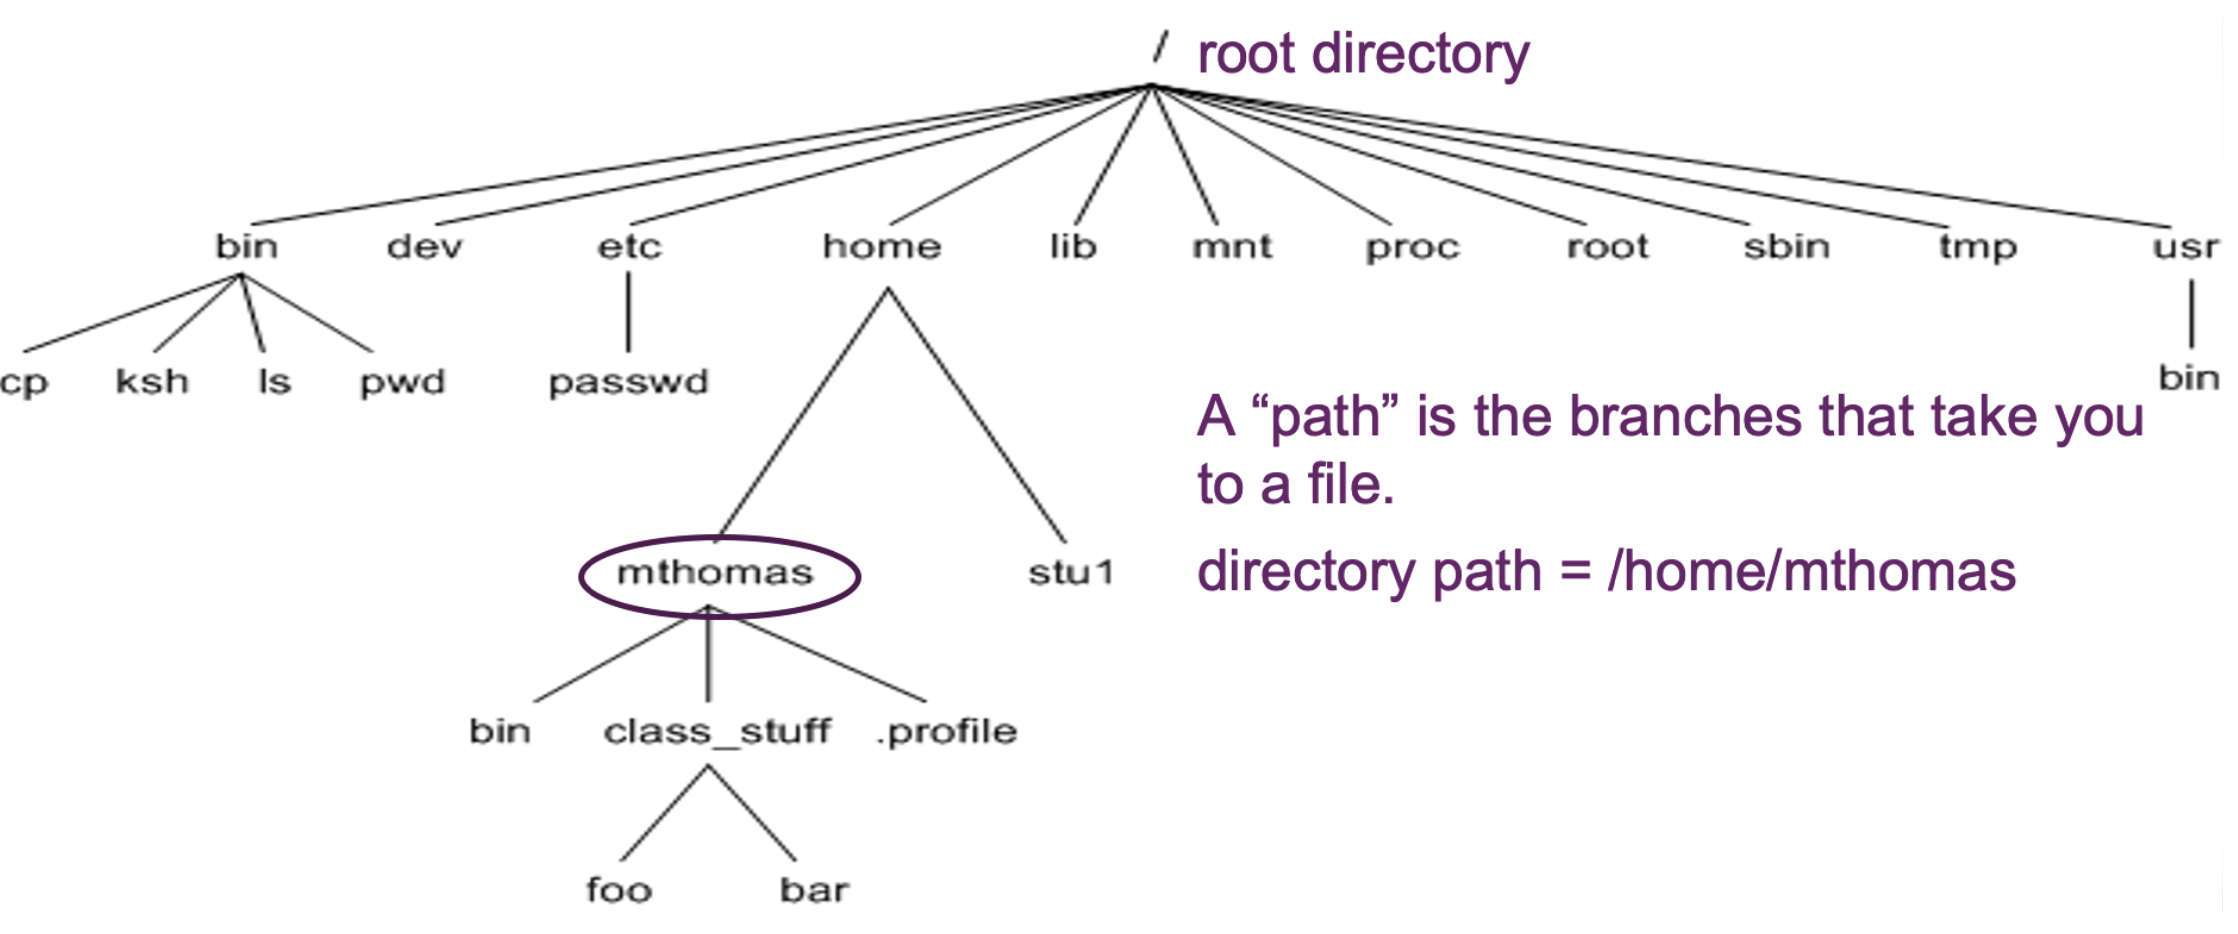
\includegraphics[width=1\textwidth,height=\textheight]{./Figures/DirectoryStructure.png}

In a Finder window, you would see this:

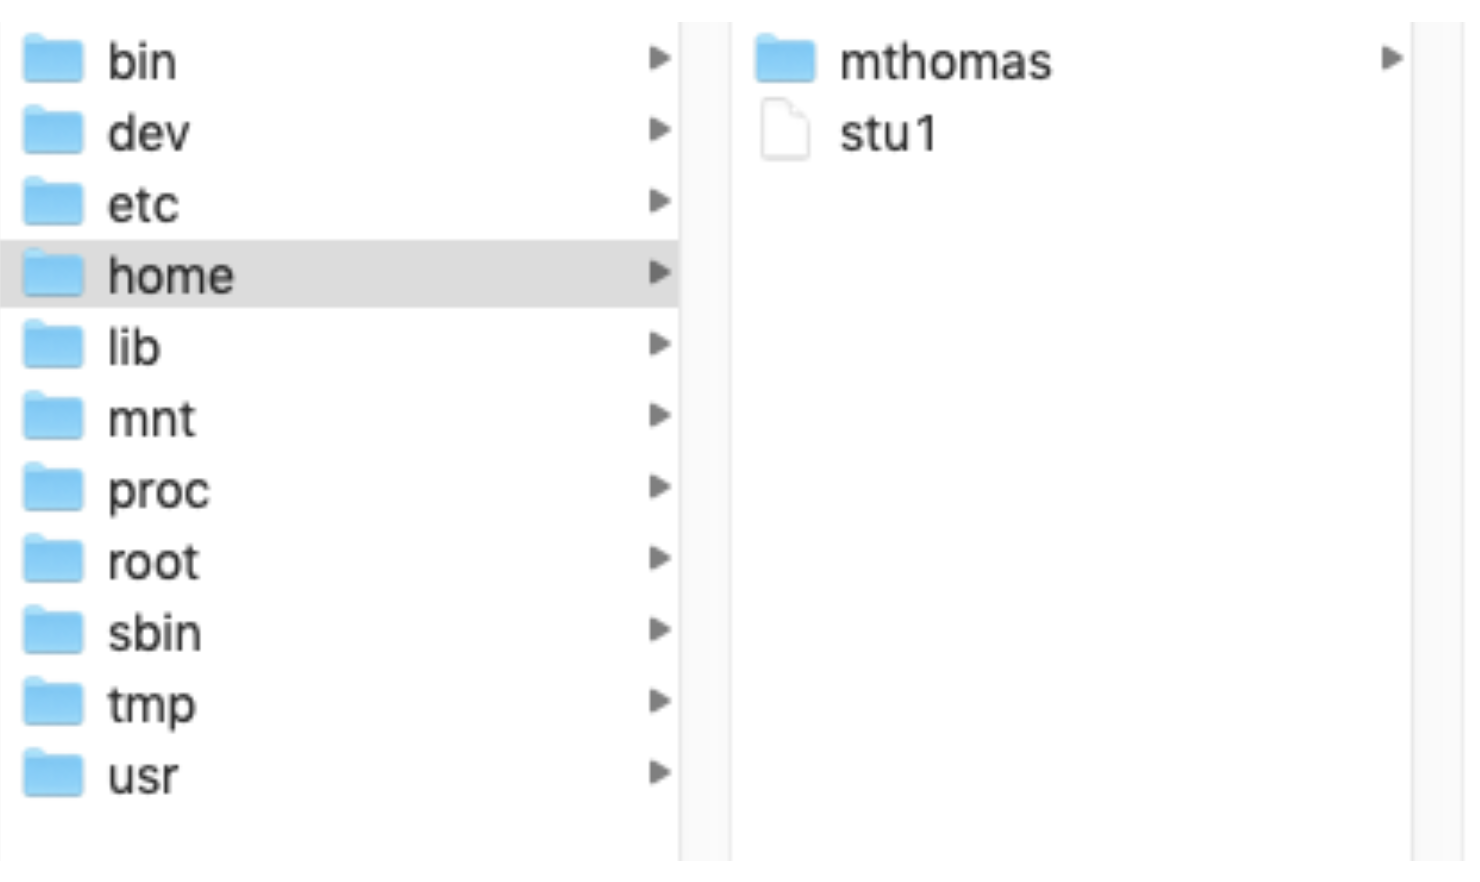
\includegraphics[width=0.6\textwidth,height=\textheight]{./Figures/FinderWindow.png}

\hypertarget{find-the-shell-in-system-youll-use-to-log-into-the-ncgrs-server}{%
\section{Find the shell in system you'll use to log into the NCGR's server}\label{find-the-shell-in-system-youll-use-to-log-into-the-ncgrs-server}}

\begin{itemize}
\tightlist
\item
  For \textbf{Windows}: search for MobaXterm from the start menu.

  \begin{itemize}
  \tightlist
  \item
    It may be useful to drag the terminal icon to the \textbf{desktop} for easier access in the future.
  \end{itemize}
\item
  For \textbf{Mac}: search for ``terminal'' in the bar located in the Launchpad (rocket icon in the taskbar).

  \begin{itemize}
  \tightlist
  \item
    It may be useful to drag the terminal icon into the \textbf{Dock} for easier access in the future.
  \end{itemize}
\end{itemize}

\hypertarget{log-on-to-logrus-server}{%
\section{Log on to logrus server}\label{log-on-to-logrus-server}}

Enter the following command to log on to logrus:

\begin{itemize}
\tightlist
\item
  substitute \textbf{your} personal username in for ``username''
\end{itemize}

\begin{verbatim}
ssh -p 44111 username@gateway.training.ncgr.org
\end{verbatim}

Notes:

\begin{itemize}
\tightlist
\item
  Because we're logging in remotely, the -p option is required to specify port 44111.
\item
  If you're prompted to confirm the connection, say ``yes'', then enter your password.
\end{itemize}

\hypertarget{now-that-i-logged-on-where-am-i}{%
\section{Now that I logged on, where am I?}\label{now-that-i-logged-on-where-am-i}}

You're at the command line interface of the logrus analysis server!

To the left of the command prompt, you should see something like this:

\begin{itemize}
\tightlist
\item
  {[}\href{mailto:eprice@logrus}{\nolinkurl{eprice@logrus}} \textasciitilde{]}\$
\end{itemize}

Command \textbf{output} is shown after the ``\#\#'' in this document.

\hypertarget{part-i-basic-topics}{%
\section{Part I: Basic Topics}\label{part-i-basic-topics}}

\hypertarget{understanding-directories}{%
\subsection{Understanding Directories}\label{understanding-directories}}

print working directory (pwd), mkdir (make directory), and list contents (ls)

\begin{verbatim}
pwd
\end{verbatim}

\begin{verbatim}
## /home/eprice
\end{verbatim}

\begin{itemize}
\tightlist
\item
  This is your ``home'' directory.
\end{itemize}

Now, create a dir under your home directory for this linux class:

\begin{verbatim}
mkdir linuxc

ls
\end{verbatim}

\begin{verbatim}
## linuxc
\end{verbatim}

\hypertarget{listing-options}{%
\subsection{Listing options}\label{listing-options}}

using the ls command

\begin{itemize}
\tightlist
\item
  \textbf{l}ong list:
\end{itemize}

\begin{verbatim}
ls -l
\end{verbatim}

\begin{verbatim}
## total 4
## drwxrwxr-x 2 eprice eprice 4096 Aug 17 22:50 linuxc
\end{verbatim}

\begin{itemize}
\tightlist
\item
  \textbf{l}ong list, by \textbf{t}ime, \textbf{r}everse order -old to new:
\end{itemize}

\begin{verbatim}
ls -ltr
\end{verbatim}

\begin{verbatim}
## total 4
## drwxrwxr-x 2 eprice eprice 4096 Aug 17 22:50 linuxc
\end{verbatim}

\hypertarget{navigation}{%
\subsection{Navigation}\label{navigation}}

\begin{enumerate}
\def\labelenumi{\arabic{enumi})}
\tightlist
\item
  ``\textbf{c}hange \textbf{d}irectory'' to the directory you made
\end{enumerate}

\begin{itemize}
\tightlist
\item
  where \textasciitilde{} is shorthand for your home directory
\end{itemize}

\begin{verbatim}
cd ~/linuxc

pwd
\end{verbatim}

\begin{verbatim}
## /home/eprice/linuxc
\end{verbatim}

\hypertarget{files-creating-with-touch-command}{%
\subsection{Files: creating with touch command}\label{files-creating-with-touch-command}}

\begin{enumerate}
\def\labelenumi{\arabic{enumi})}
\tightlist
\item
  Create a file
\end{enumerate}

\begin{verbatim}
touch newfile.txt

ls -l
\end{verbatim}

\begin{verbatim}
## total 0
## -rw-rw-r-- 1 eprice eprice 0 Aug 17 22:50 newfile.txt
\end{verbatim}

\begin{enumerate}
\def\labelenumi{\arabic{enumi})}
\setcounter{enumi}{1}
\tightlist
\item
  Change to your home dir
\end{enumerate}

\begin{verbatim}
cd ~ 

pwd
\end{verbatim}

\begin{verbatim}
## /home/eprice
\end{verbatim}

\hypertarget{history-command}{%
\subsection{History command}\label{history-command}}

lists the commands you have entered

\begin{verbatim}
history
\end{verbatim}

\begin{verbatim}
## 17 ls -ltr
## 18 cd ../linuxc
## 19 ls -ltr
## 20 history
\end{verbatim}

Scroll through recent commands with the up and down arrows.

To perform a command from the list by number:

\begin{verbatim}
!17
\end{verbatim}

To perform the last command you made:

\begin{verbatim}
!!
\end{verbatim}

\hypertarget{files-creating-by-redirecting-standard-out}{%
\subsection{Files: creating by redirecting standard out}\label{files-creating-by-redirecting-standard-out}}

redirect operator \textbf{\textgreater{}}

To send output to a file instead of standard out:

\begin{itemize}
\tightlist
\item
  standard out is just the terminal
\end{itemize}

\begin{verbatim}
history > history.txt

ls -l
\end{verbatim}

\begin{verbatim}
## total 4
## -rw-rw-r-- 1 eprice eprice 0    Aug 17 22:50 history.txt
## drwxrwxr-x 2 eprice eprice 4096 Aug 17 22:50 linuxc
\end{verbatim}

\begin{verbatim}
cat history.txt
\end{verbatim}

\begin{verbatim}
## 17 ls -ltr
## 18 cd ../linuxc
## 19 ls -ltr
## 20 history
## 21 ls -ltr
## 20 history > history
\end{verbatim}

Now you have a file with your commands!

\hypertarget{file-name-completion-with-tab}{%
\subsection{File name completion with tab}\label{file-name-completion-with-tab}}

To autocomplete remainder of file name instead of typing it all in:

\begin{itemize}
\tightlist
\item
  cat h\ldots(press tab)

  \begin{itemize}
  \tightlist
  \item
    cat history
  \end{itemize}
\item
  prevents typos and saves time
\end{itemize}

\hypertarget{files-moving-files-from-one-filename-to-another}{%
\subsection{Files: moving files from one filename to another}\label{files-moving-files-from-one-filename-to-another}}

\textbf{m}o\textbf{v}ing ``mv'' command

\hypertarget{syntax-mv-sourcefilename-destinationfilename}{%
\subsubsection*{Syntax: mv sourcefilename destinationfilename}\label{syntax-mv-sourcefilename-destinationfilename}}
\addcontentsline{toc}{subsubsection}{Syntax: mv sourcefilename destinationfilename}

\begin{verbatim}
mv history.txt history_file.txt

ls -l
\end{verbatim}

\begin{verbatim}
## total 4
## -rw-rw-r-- 1 eprice eprice 0    Aug 17 22:50 history_file.txt 
## drwxrwxr-x 2 eprice eprice 4096 Aug 17 22:50 linuxc
\end{verbatim}

\hypertarget{files-copying-files-from-one-filename-to-another}{%
\subsection{Files: copying files from one filename to another}\label{files-copying-files-from-one-filename-to-another}}

\textbf{c}o\textbf{p}ying ``cp'' command

\hypertarget{syntax-cp-sourcefilename-destinationfilename}{%
\subsubsection*{Syntax: cp sourcefilename destinationfilename}\label{syntax-cp-sourcefilename-destinationfilename}}
\addcontentsline{toc}{subsubsection}{Syntax: cp sourcefilename destinationfilename}

\begin{enumerate}
\def\labelenumi{\arabic{enumi})}
\tightlist
\item
  Change back to the linuxc directory:
\end{enumerate}

\begin{verbatim}
cd ~/linuxc
\end{verbatim}

\begin{enumerate}
\def\labelenumi{\arabic{enumi})}
\setcounter{enumi}{1}
\tightlist
\item
  Make a ``back up'' copy of a file in your working directory:
\end{enumerate}

\begin{verbatim}
cp ~/linuxc/newfile.txt newfile_bu.txt
\end{verbatim}

\begin{enumerate}
\def\labelenumi{\arabic{enumi})}
\setcounter{enumi}{2}
\tightlist
\item
  Check if the newly copied file is there:
\end{enumerate}

\begin{verbatim}
ls
\end{verbatim}

\begin{verbatim}
## newfile_bu.txt
## newfile.txt
\end{verbatim}

\hypertarget{files-securely-copying-files-between-your-laptop-and-logrus}{%
\subsection{Files: securely copying files between your laptop and logrus}\label{files-securely-copying-files-between-your-laptop-and-logrus}}

\textbf{s}ecure \textbf{c}o\textbf{p}y ``scp'' command

\begin{itemize}
\tightlist
\item
  a secure way to copy files to/from a server while you're working on an outside network

  \begin{itemize}
  \tightlist
  \item
    like from your home or starbucks to logrus and vice versa
  \end{itemize}
\end{itemize}

\hypertarget{syntax-scp-options-sourcepath-destinationpath}{%
\subsubsection*{Syntax: scp {[}options{]} sourcepath destinationpath}\label{syntax-scp-options-sourcepath-destinationpath}}
\addcontentsline{toc}{subsubsection}{Syntax: scp {[}options{]} sourcepath destinationpath}

\begin{enumerate}
\def\labelenumi{\arabic{enumi})}
\tightlist
\item
  Create a file to copy
\end{enumerate}

\begin{verbatim}
touch scp_test.txt
\end{verbatim}

\begin{enumerate}
\def\labelenumi{\arabic{enumi})}
\setcounter{enumi}{1}
\tightlist
\item
\end{enumerate}

\begin{itemize}
\tightlist
\item
  \textbf{Mac} users

  \begin{itemize}
  \tightlist
  \item
    open a \textbf{local} terminal
  \item
    do \textbf{not} connect it to logrus
  \end{itemize}
\item
  \textbf{Windows} users

  \begin{itemize}
  \tightlist
  \item
    open a new MobaXterm session (shell)
  \end{itemize}
\end{itemize}

\begin{enumerate}
\def\labelenumi{\arabic{enumi})}
\setcounter{enumi}{2}
\tightlist
\item
  Run the scp command from your \textbf{local} terminal window:
\end{enumerate}

\begin{itemize}
\tightlist
\item
  to \textbf{download} the file \textbf{to your computer} from logrus
\item
  the last period means that the destination is your working directory
\end{itemize}

\begin{verbatim}
scp -P 44111 <user>@gateway.training.ncgr.org:~/linuxc/scp_test.txt .
\end{verbatim}

Note: When you designate a port with secure copy (scp), you use a capital P.

You will be prompted for your logrus password if not using MobaXterm.

\begin{enumerate}
\def\labelenumi{\arabic{enumi})}
\setcounter{enumi}{3}
\item
  Check to see if the file you copied from logrus is on \textbf{your} computer!
\item
  Now \textbf{upload} a file \textbf{to logrus} from your computer
\end{enumerate}

\begin{itemize}
\tightlist
\item
  Again, run the scp command from your \textbf{local} terminal window:
\end{itemize}

\begin{verbatim}
scp -P 44111 scp_test.txt <user>@gateway.training.ncgr.org:~/linuxc
\end{verbatim}

\begin{enumerate}
\def\labelenumi{\arabic{enumi})}
\setcounter{enumi}{5}
\tightlist
\item
  Check to see if the file you copied from your computer is on \textbf{logrus}!
\end{enumerate}

\hypertarget{files-and-directories-removing-files-is-deleting-files}{%
\subsection{Files and directories: removing files is deleting files}\label{files-and-directories-removing-files-is-deleting-files}}

\textbf{r}e\textbf{m}oving ``rm'' command

\hypertarget{syntax-rm-options-filename}{%
\subsubsection*{Syntax: rm {[}options{]} filename}\label{syntax-rm-options-filename}}
\addcontentsline{toc}{subsubsection}{Syntax: rm {[}options{]} filename}

\begin{verbatim}
rm -i newfile_bu.txt
\end{verbatim}

\begin{verbatim}
## rm: remove regular empty file newfile_bu.txt?
\end{verbatim}

Enter ``yes'' or ``y'' in response to the question:

\begin{verbatim}
yes

ls -l
\end{verbatim}

\begin{verbatim}
## total 0
## -rw-rw-r-- 1 eprice eprice 0 Aug 17 22:50 newfile.txt
\end{verbatim}

At this point everyone should have the above in their linuxc class directory.

\hypertarget{tool-box-how-to-abort-a-commandprocess}{%
\subsection{Tool box: How to abort a command/process}\label{tool-box-how-to-abort-a-commandprocess}}

Hold ``control'' key then hit ``c'' key, then release.

\begin{itemize}
\tightlist
\item
  Control-key often referred to as CTRL.
\end{itemize}

Let's say you type a command and nothing happens; it hangs.
This can happen when the syntax doesn't make sense.
Good time for CTRL c

\begin{verbatim}
cat
\end{verbatim}

If you can't execute commands, then CTRL c

\begin{verbatim}
## ^C
\end{verbatim}

You should be returned to your prompt: {[}\href{mailto:username@logrus}{\nolinkurl{username@logrus}} linuxc{]}\$

\hypertarget{part-ii-advanced-topics}{%
\section{PART II: Advanced Topics}\label{part-ii-advanced-topics}}

\hypertarget{files-symbolic-links-and-the-soft-link--s}{%
\subsection{Files: Symbolic links and the soft link (-s)}\label{files-symbolic-links-and-the-soft-link--s}}

\hypertarget{syntax-ln--s-fileyouwanttolinkpointto-nameyouwanttogiveit}{%
\subsubsection*{Syntax: ln -s FileYouWantToLink/PointTo NameYouWantToGiveIt}\label{syntax-ln--s-fileyouwanttolinkpointto-nameyouwanttogiveit}}
\addcontentsline{toc}{subsubsection}{Syntax: ln -s FileYouWantToLink/PointTo NameYouWantToGiveIt}

\begin{verbatim}
ln -s /home/eprice/covid.fasta covid.fasta

ls -l
\end{verbatim}

\begin{verbatim}
## total 0
## lrwxrwxrwx 1 eprice eprice 26 Aug 17 22:50 covid.fasta -> /home/eprice/covid.fasta 
## -rw-rw-r-- 1 eprice Aug 17 22:50 newfile.txt
\end{verbatim}

\hypertarget{understanding-a-fasta-file-format}{%
\subsection{Understanding a fasta file format}\label{understanding-a-fasta-file-format}}

Fasta files (.fasta or .fa) contain one or more sequences, each preceded by a \textbf{header} starting with ``\textgreater{}''.

Show only the \textbf{first 10 lines} of a file with ``head'' command:

\begin{verbatim}
head covid.fasta
\end{verbatim}

\begin{verbatim}
## >NC_045512.2 |Severe acute respiratory syndrome coronavirus 2 isolate Wuhan-Hu-1, co
## ATTAAAGGTTTATACCTTCCCAGGTAACAAACCAACCAACTTTCGATCTCTTGTAGATCT
## GTTCTCTAAACGAACTTTAAAATCTGTGTGGCTGTCACTCGGCTGCATGCTTAGTGCACT
## CACGCAGTATAATTAATAACTAATTACTGTCGTTGACAGGACACGAGTAACTCGTCTATC
## TTCTGCAGGCTGCTTACGGTTTCGTCCGTGTTGCAGCCGATCATCAGCACATCTAGGTTT
## CGTCCGGGTGTGACCGAAAGGTAAGATGGAGAGCCTTGTCCCTGGTTTCAACGAGAAAAC
## ACACGTCCAACTCAGTTTGCCTGTTTTACAGGTTCGCGACGTGCTCGTACGTGGCTTTGG
## AGACTCCGTGGAGGAGGTCTTATCAGAGGCACGTCAACATCTTAAAGATGGCACTTGTGG
## CTTAGTAGAAGTTGAAAAAGGCGTTTTGCCTCAACTTGAACAGCCCTATGTGTTCATCAA
## ACGTTCGGATGCTCGAACTGCACCTCATGGTCATGTTATGGTTGAGCTGGTAGCAGAACT
\end{verbatim}

Now show only the \textbf{last 10 lines} of a file using the ``tail'' command:

\begin{verbatim}
tail covid.fasta
\end{verbatim}

\begin{verbatim}
## TATTGACGCATACAAAACATTCCCACCAACAGAGCCTAAAAAGGACAAAAAGAAGAAGGC
## TGATGAAACTCAAGCCTTACCGCAGAGACAGAAGAAACAGCAAACTGTGACTCTTCTTCC
## TGCTGCAGATTTGGATGATTTCTCCAAACAATTGCAACAATCCATGAGCAGTGCTGACTC
## AACTCAGGCCTAAACTCATGCAGACCACACAAGGCAGATGGGCTATATAAACGTTTTCGC
## TTTTCCGTTTACGATATATAGTCTACTCTTGTGCAGAATGAATTCTCGTAACTACATAGC
## ACAAGTAGATGTAGTTAACTTTAATCTCACATAGCAATCTTTAATCAGTGTGTAACATTA
## GGGAGGACTTGAAAGAGCCACCACATTTTCACCGAGGCCACGCGGAGTACGATCGAGTGT
## ACAGTGAACAATGCTAGGGAGAGCTGCCTATATGGAAGAGCCCTAATGTGTAAAATTAAT
## TTTAGTAGTGCTATCCCCATGTGATTTTAATAGCTTCTTAGGAGAATGACAAAAAAAAAA
## AAAAAAAAAAAAAAAAAAAAAAA
\end{verbatim}

\hypertarget{the-pipe-operator-will-redirect-output-of-a-command-to-another-command.}{%
\subsubsection*{The pipe operator will redirect output of a command to another command.}\label{the-pipe-operator-will-redirect-output-of-a-command-to-another-command.}}
\addcontentsline{toc}{subsubsection}{The pipe operator will redirect output of a command to another command.}

Use the pipe operator to redirect ``cat'' output to ``head'':

\begin{itemize}
\tightlist
\item
  The symbol ``\textbar{}'' denotes a pipe
\end{itemize}

\begin{verbatim}
cat covid.fasta | head
\end{verbatim}

\begin{verbatim}
## >NC_045512.2 |Severe acute respiratory syndrome coronavirus 2 isolate Wuhan-Hu-1, co
## ATTAAAGGTTTATACCTTCCCAGGTAACAAACCAACCAACTTTCGATCTCTTGTAGATCT
## GTTCTCTAAACGAACTTTAAAATCTGTGTGGCTGTCACTCGGCTGCATGCTTAGTGCACT
## CACGCAGTATAATTAATAACTAATTACTGTCGTTGACAGGACACGAGTAACTCGTCTATC
## TTCTGCAGGCTGCTTACGGTTTCGTCCGTGTTGCAGCCGATCATCAGCACATCTAGGTTT
## CGTCCGGGTGTGACCGAAAGGTAAGATGGAGAGCCTTGTCCCTGGTTTCAACGAGAAAAC
## ACACGTCCAACTCAGTTTGCCTGTTTTACAGGTTCGCGACGTGCTCGTACGTGGCTTTGG
## AGACTCCGTGGAGGAGGTCTTATCAGAGGCACGTCAACATCTTAAAGATGGCACTTGTGG
## CTTAGTAGAAGTTGAAAAAGGCGTTTTGCCTCAACTTGAACAGCCCTATGTGTTCATCAA
## ACGTTCGGATGCTCGAACTGCACCTCATGGTCATGTTATGGTTGAGCTGGTAGCAGAACT
\end{verbatim}

\begin{verbatim}
cat covid.fasta | tail
\end{verbatim}

\begin{verbatim}
## TATTGACGCATACAAAACATTCCCACCAACAGAGCCTAAAAAGGACAAAAAGAAGAAGGC
## TGATGAAACTCAAGCCTTACCGCAGAGACAGAAGAAACAGCAAACTGTGACTCTTCTTCC
## TGCTGCAGATTTGGATGATTTCTCCAAACAATTGCAACAATCCATGAGCAGTGCTGACTC
## AACTCAGGCCTAAACTCATGCAGACCACACAAGGCAGATGGGCTATATAAACGTTTTCGC
## TTTTCCGTTTACGATATATAGTCTACTCTTGTGCAGAATGAATTCTCGTAACTACATAGC
## ACAAGTAGATGTAGTTAACTTTAATCTCACATAGCAATCTTTAATCAGTGTGTAACATTA
## GGGAGGACTTGAAAGAGCCACCACATTTTCACCGAGGCCACGCGGAGTACGATCGAGTGT
## ACAGTGAACAATGCTAGGGAGAGCTGCCTATATGGAAGAGCCCTAATGTGTAAAATTAAT
## TTTAGTAGTGCTATCCCCATGTGATTTTAATAGCTTCTTAGGAGAATGACAAAAAAAAAA
## AAAAAAAAAAAAAAAAAAAAAAA
\end{verbatim}

\hypertarget{understanding-fastq-fq-file-format}{%
\subsection{Understanding fastq (fq) file format}\label{understanding-fastq-fq-file-format}}

Fastq files contain sequence reads and associated \textbf{meta data}.

\begin{verbatim}
ln -s /home/fds/unix_basics/SP1.fq SP1.fq

ls -ltr
\end{verbatim}

\begin{verbatim}
## total 0
## -rw-rw-r-- 1 eprice eprice 0 Aug 17 22:50 newfile.txt
## lrwxrwxrwx 1 eprice eprice 26 Aug 17 22:50 covid.fasta -> /home/eprice/covid.fasta 
## lrwxrwxrwx 1 eprice eprice Aug 17 22:50 SP1.fq -> /home/fds/unix_basics/SP1.fq
\end{verbatim}

Tail the last 4 lines:

\begin{verbatim}
tail -n 4 SP1.fq
\end{verbatim}

\begin{verbatim}
## @cluster_834:UMI_TTAAGG
## AGGGTGGGGGATCACATTTATTGTATTGAGG 
## +
## =A=@AB===>4?A=??EEB?EB@C?ECB=A?
\end{verbatim}

A fastq file has 4 lines per record:

\begin{itemize}
\tightlist
\item
  The header; starts with ``@''
\item
  The sequence
\item
  Throwaway line; begins with ``+''
\item
  Phred-scaled quality scores
\end{itemize}

\hypertarget{what-is-the-difference-between-this-and-a-fasta-file}{%
\paragraph*{What is the difference between this and a fasta file?}\label{what-is-the-difference-between-this-and-a-fasta-file}}
\addcontentsline{toc}{paragraph}{What is the difference between this and a fasta file?}

\hypertarget{using-grep-global-regular-expression-print-to-extract-metrics}{%
\subsection{Using grep (global regular expression print) to extract metrics}\label{using-grep-global-regular-expression-print-to-extract-metrics}}

Grep will output the lines containing a provided expression.

\hypertarget{syntax-grep-options-expression-filename}{%
\subsubsection*{Syntax: grep {[}options{]} ``expression'' filename}\label{syntax-grep-options-expression-filename}}
\addcontentsline{toc}{subsubsection}{Syntax: grep {[}options{]} ``expression'' filename}

\begin{verbatim}
grep ">" covid.fasta
\end{verbatim}

\begin{verbatim}
## >NC_045512.2 |Severe acute respiratory syndrome coronavirus 2 isolate Wuhan-Hu-1, co
## >MT627325.1 |Severe acute respiratory syndrome coronavirus 2 isolate SARS-CoV-2/huma
## >MT622319.1 |Severe acute respiratory syndrome coronavirus 2 isolate SARS-CoV-2/huma
## >MT568634.1 |Severe acute respiratory syndrome coronavirus 2 isolate SARS-CoV-2/huma
## >MT568635.1 |Severe acute respiratory syndrome coronavirus 2 isolate SARS-CoV-2/huma
## >MT568636.1 |Severe acute respiratory syndrome coronavirus 2 isolate SARS-CoV-2/huma
## >MT568637.1 |Severe acute respiratory syndrome coronavirus 2 isolate SARS-CoV-2/huma
## >MT568638.1 |Severe acute respiratory syndrome coronavirus 2 isolate SARS-CoV-2/huma
## >MT568639.1 |Severe acute respiratory syndrome coronavirus 2 isolate SARS-CoV-2/huma
## >MT568640.1 |Severe acute respiratory syndrome coronavirus 2 isolate SARS-CoV-2/huma
## >MT568641.1 |Severe acute respiratory syndrome coronavirus 2 isolate SARS-CoV-2/huma
## >MT407649.1 |Severe acute respiratory syndrome coronavirus 2 isolate SARS-CoV-2/huma
## >MT407650.1 |Severe acute respiratory syndrome coronavirus 2 isolate SARS-CoV-2/huma
## >MT407651.1 |Severe acute respiratory syndrome coronavirus 2 isolate SARS-CoV-2/huma
## >MT407652.1 |Severe acute respiratory syndrome coronavirus 2 isolate SARS-CoV-2/huma
## >MT407653.1 |Severe acute respiratory syndrome coronavirus 2 isolate SARS-CoV-2/huma
## >MT407654.1 |Severe acute respiratory syndrome coronavirus 2 isolate SARS-CoV-2/huma
## >MT407655.1 |Severe acute respiratory syndrome coronavirus 2 isolate SARS-CoV-2/huma
## >MT407656.1 |Severe acute respiratory syndrome coronavirus 2 isolate SARS-CoV-2/huma
## >MT407657.1 |Severe acute respiratory syndrome coronavirus 2 isolate SARS-CoV-2/huma
## >MT407658.1 |Severe acute respiratory syndrome coronavirus 2 isolate SARS-CoV-2/huma
## >MT407659.1 |Severe acute respiratory syndrome coronavirus 2 isolate SARS-CoV-2/huma
## >MT534630.1 |Severe acute respiratory syndrome coronavirus 2 isolate SARS-CoV-2/huma
## >MT510727.1 |Severe acute respiratory syndrome coronavirus 2 isolate SARS-CoV-2/huma
## >MT510728.1 |Severe acute respiratory syndrome coronavirus 2 isolate SARS-CoV-2/huma
## >MT079843.1 |Severe acute respiratory syndrome coronavirus 2 isolate SARS-CoV-2/huma
## >MT079844.1 |Severe acute respiratory syndrome coronavirus 2 isolate SARS-CoV-2/huma
## >MT079845.1 |Severe acute respiratory syndrome coronavirus 2 isolate SARS-CoV-2/huma
## >MT079846.1 |Severe acute respiratory syndrome coronavirus 2 isolate SARS-CoV-2/huma
## >MT079847.1 |Severe acute respiratory syndrome coronavirus 2 isolate SARS-CoV-2/huma
## >MT079848.1 |Severe acute respiratory syndrome coronavirus 2 isolate SARS-CoV-2/huma
## >MT079849.1 |Severe acute respiratory syndrome coronavirus 2 isolate SARS-CoV-2/huma
## >MT079850.1 |Severe acute respiratory syndrome coronavirus 2 isolate SARS-CoV-2/huma
## >MT079851.1 |Severe acute respiratory syndrome coronavirus 2 isolate SARS-CoV-2/huma
## >MT079852.1 |Severe acute respiratory syndrome coronavirus 2 isolate SARS-CoV-2/huma
## >MT079853.1 |Severe acute respiratory syndrome coronavirus 2 isolate SARS-CoV-2/huma
## >MT079854.1 |Severe acute respiratory syndrome coronavirus 2 isolate SARS-CoV-2/huma
## >MT446312.1 |Severe acute respiratory syndrome coronavirus 2 isolate SARS-CoV-2/huma
## >MT412134.1 |Severe acute respiratory syndrome coronavirus 2 isolate SARS-CoV-2/huma
## >MT396241.1 |Severe acute respiratory syndrome coronavirus 2 isolate SARS-CoV-2/huma
## >MT039874.1 |Severe acute respiratory syndrome coronavirus 2 isolate SARS-CoV-2/huma
## >MT281577.1 |Severe acute respiratory syndrome coronavirus 2 isolate SARS-CoV-2/huma
## >MT291826.1 |Severe acute respiratory syndrome coronavirus 2 isolate SARS-CoV-2/huma
## >MT291827.1 |Severe acute respiratory syndrome coronavirus 2 isolate SARS-CoV-2/huma
## >MT291828.1 |Severe acute respiratory syndrome coronavirus 2 isolate SARS-CoV-2/huma
## >MT291829.1 |Severe acute respiratory syndrome coronavirus 2 isolate SARS-CoV-2/huma
## >MT291830.1 |Severe acute respiratory syndrome coronavirus 2 isolate SARS-CoV-2/huma
## >MT291831.1 |Severe acute respiratory syndrome coronavirus 2 isolate SARS-CoV-2/huma
## >MT291832.1 |Severe acute respiratory syndrome coronavirus 2 isolate SARS-CoV-2/huma
## >MT291833.1 |Severe acute respiratory syndrome coronavirus 2 isolate SARS-CoV-2/huma
## >MT291834.1 |Severe acute respiratory syndrome coronavirus 2 isolate SARS-CoV-2/huma
## >MT291835.2 |Severe acute respiratory syndrome coronavirus 2 isolate SARS-CoV-2/huma
## >MT291836.1 |Severe acute respiratory syndrome coronavirus 2 isolate SARS-CoV-2/huma
## >MT259226.1 |Severe acute respiratory syndrome coronavirus 2 isolate SARS-CoV-2/huma
## >MT259227.1 |Severe acute respiratory syndrome coronavirus 2 isolate SARS-CoV-2/huma
## >MT259228.1 |Severe acute respiratory syndrome coronavirus 2 isolate SARS-CoV-2/huma
## >MT259229.1 |Severe acute respiratory syndrome coronavirus 2 isolate SARS-CoV-2/huma
## >MT259230.1 |Severe acute respiratory syndrome coronavirus 2 isolate SARS-CoV-2/huma
## >MT259231.1 |Severe acute respiratory syndrome coronavirus 2 isolate SARS-CoV-2/huma
## >MT253696.1 |Severe acute respiratory syndrome coronavirus 2 isolate SARS-CoV-2/huma
## >MT253697.1 |Severe acute respiratory syndrome coronavirus 2 isolate SARS-CoV-2/huma
## >MT253698.1 |Severe acute respiratory syndrome coronavirus 2 isolate SARS-CoV-2/huma
## >MT253699.1 |Severe acute respiratory syndrome coronavirus 2 isolate SARS-CoV-2/huma
## >MT253700.1 |Severe acute respiratory syndrome coronavirus 2 isolate SARS-CoV-2/huma
## >MT253701.1 |Severe acute respiratory syndrome coronavirus 2 isolate SARS-CoV-2/huma
## >MT253702.1 |Severe acute respiratory syndrome coronavirus 2 isolate SARS-CoV-2/huma
## >MT253703.1 |Severe acute respiratory syndrome coronavirus 2 isolate SARS-CoV-2/huma
## >MT253704.1 |Severe acute respiratory syndrome coronavirus 2 isolate SARS-CoV-2/huma
## >MT253705.1 |Severe acute respiratory syndrome coronavirus 2 isolate SARS-CoV-2/huma
## >MT253706.1 |Severe acute respiratory syndrome coronavirus 2 isolate SARS-CoV-2/huma
## >MT253707.1 |Severe acute respiratory syndrome coronavirus 2 isolate SARS-CoV-2/huma
## >MT253708.1 |Severe acute respiratory syndrome coronavirus 2 isolate SARS-CoV-2/huma
## >MT253709.1 |Severe acute respiratory syndrome coronavirus 2 isolate SARS-CoV-2/huma
## >MT253710.1 |Severe acute respiratory syndrome coronavirus 2 isolate SARS-CoV-2/huma
## >MT226610.1 |Severe acute respiratory syndrome coronavirus 2 isolate SARS-CoV-2/huma
## >MT121215.1 |Severe acute respiratory syndrome coronavirus 2 isolate SARS-CoV-2/huma
## >MT135041.1 |Severe acute respiratory syndrome coronavirus 2 isolate SARS-CoV-2/huma
## >MT135042.1 |Severe acute respiratory syndrome coronavirus 2 isolate SARS-CoV-2/huma
## >MT135043.1 |Severe acute respiratory syndrome coronavirus 2 isolate SARS-CoV-2/huma
## >MT135044.1 |Severe acute respiratory syndrome coronavirus 2 isolate SARS-CoV-2/huma
## >MT123290.1 |Severe acute respiratory syndrome coronavirus 2 isolate SARS-CoV-2/huma
## >MT123291.2 |Severe acute respiratory syndrome coronavirus 2 isolate SARS-CoV-2/huma
## >MT123292.2 |Severe acute respiratory syndrome coronavirus 2 isolate SARS-CoV-2/huma
## >MT123293.2 |Severe acute respiratory syndrome coronavirus 2 isolate SARS-CoV-2/huma
## >MT093631.2 |Severe acute respiratory syndrome coronavirus 2 isolate SARS-CoV-2/huma
## >MT049951.1 |Severe acute respiratory syndrome coronavirus 2 isolate SARS-CoV-2/huma
## >MT039873.1 |Severe acute respiratory syndrome coronavirus 2 isolate HZ-1, complete
## >MT019529.1 |Severe acute respiratory syndrome coronavirus 2 isolate BetaCoV/Wuhan/I
## >MT019530.1 |Severe acute respiratory syndrome coronavirus 2 isolate BetaCoV/Wuhan/I
## >MT019531.1 |Severe acute respiratory syndrome coronavirus 2 isolate BetaCoV/Wuhan/I
## >MT019532.1 |Severe acute respiratory syndrome coronavirus 2 isolate BetaCoV/Wuhan/I
## >MT019533.1 |Severe acute respiratory syndrome coronavirus 2 isolate BetaCoV/Wuhan/I
## >MN996527.1 |Severe acute respiratory syndrome coronavirus 2 isolate WIV02, complete
## >MN996528.1 |Severe acute respiratory syndrome coronavirus 2 isolate WIV04, complete
## >MN996529.1 |Severe acute respiratory syndrome coronavirus 2 isolate WIV05, complete
## >MN996530.1 |Severe acute respiratory syndrome coronavirus 2 isolate WIV06, complete
## >MN996531.1 |Severe acute respiratory syndrome coronavirus 2 isolate WIV07, complete
## >MN988668.1 |Severe acute respiratory syndrome coronavirus 2 isolate 2019-nCoV WHU01
## >MN988669.1 |Severe acute respiratory syndrome coronavirus 2 isolate 2019-nCoV WHU02
## >MN938384.1 |Severe acute respiratory syndrome coronavirus 2 isolate 2019-nCoV_HKU-S
## >MN975262.1 |Severe acute respiratory syndrome coronavirus 2 isolate 2019-nCoV_HKU-S
## >MN908947.3 |Severe acute respiratory syndrome coronavirus 2 isolate Wuhan-Hu-1, com
\end{verbatim}

Adding the ``-c'' option counts the number of lines containing a match

\begin{itemize}
\tightlist
\item
  \textbf{not} the number of matches!
\end{itemize}

\begin{verbatim}
grep -c ">" covid.fasta
\end{verbatim}

\begin{verbatim}
## 102
\end{verbatim}

The ``-v'' option reverses the grep search, which is the first step towards finding the total length of sequences

\begin{verbatim}
grep -v ">" covid.fasta
\end{verbatim}

Use c to halt the overflow of output.

We can add in the pipe operator to redirect our output to the ``wc'' command.

The output shows the number of newline characters, followed by line count and total character count.

\begin{verbatim}
grep -v ">" covid.fasta | wc
\end{verbatim}

wc: prints newline, word, and byte counts for each file:

\begin{verbatim}
## 50812 50812 3096018
\end{verbatim}

Let's trim out the newline characters with ``tr -d'' before doing the word count:

\begin{verbatim}
grep -v ">" covid.fasta | tr -d ’\n’ | wc
\end{verbatim}

\begin{verbatim}
##       0       1 3045206
\end{verbatim}

\hypertarget{working-with-compressed-files}{%
\subsection{Working with compressed files}\label{working-with-compressed-files}}

Powerful Z commands (zcat)

\begin{itemize}
\tightlist
\item
  p.~1 of 2
\end{itemize}

Let's copy another file:

\begin{verbatim}
cp /home/fds/unix_basics/table1.txt.gz /home/<user>/linuxczcat table1.txt.gz
\end{verbatim}

\begin{verbatim}
## 1, Justin Timberlake, Title 545, Price $7.30
## 2, Taylor Swift, Title 723, Price $7.90
## 3, Mick Jagger, Title 610, Price $7.90
## 4, Lady Gaga, Title 118, Price $7.30
## 5, Johnny Cash, Title 482, Price $6.50
## 6, Elvis Presley, Title 335, Price $7.30
## 7, John Lennon, Title 271, Price $7.90
## 8, Michael Jackson, Title 373, Price $5.50
\end{verbatim}

\begin{verbatim}
zgrep "Jagger" table1.txt.gz
\end{verbatim}

\begin{verbatim}
## 3, Mick Jagger, Title 610, Price $7.90
\end{verbatim}

!! = last command

:s = substitute /word1/with word2

\begin{verbatim}
!!:s/Jagger/John
\end{verbatim}

\begin{verbatim}
## 5, Johnny Cash, Title 482, Price $6.50
## 7, John Lennon, Title 271, Price $7.90
\end{verbatim}

\hypertarget{start-and-end-symbols}{%
\subsection{Start \^{} and end \$ symbols}\label{start-and-end-symbols}}

Powerful Z commands (zgrep)

\begin{itemize}
\tightlist
\item
  p.~2 of 2
\end{itemize}

Display all the lines that start with 8:

\begin{verbatim}
zgrep "^8" table1.txt.gz
\end{verbatim}

\begin{verbatim}
## 8, Michael Jackson, Title 373, Price $5.50
\end{verbatim}

Display all the lines that end with 50:

\begin{verbatim}
zgrep "50$" table1.txt.gz
\end{verbatim}

\begin{verbatim}
## 5, Johnny Cash, Title 482, Price $6.50
## 8, Michael Jackson, Title 373, Price $5.50
\end{verbatim}

\hypertarget{files-parsing-and-creating-data-subsets}{%
\subsection{Files: parsing and creating data-subsets}\label{files-parsing-and-creating-data-subsets}}

p.1 of 5

Be sure you are in linuxc directory (as usual)

AWK command

\begin{itemize}
\tightlist
\item
  \textbf{A}ho, \textbf{W}einberger and \textbf{K}ernighan

  \begin{itemize}
  \tightlist
  \item
    the authors of the language
  \end{itemize}
\end{itemize}

General syntax:

\begin{itemize}
\tightlist
\item
  awk 'pattern \{action\}' input-file

  \begin{itemize}
  \tightlist
  \item
    output goes to standard out=terminal
  \end{itemize}
\item
  awk 'pattern \{action\}' input-file \textgreater{} output-file

  \begin{itemize}
  \tightlist
  \item
    or send to an output file
  \end{itemize}
\end{itemize}

\hypertarget{exercise}{%
\subsubsection*{Exercise:}\label{exercise}}
\addcontentsline{toc}{subsubsection}{Exercise:}

How many fields does the 1st row of table1.txt have?

Let's look at the 1st row of table1.txt:

1, Justin Timberlake, Title 545, Price \$7.30

How many fields does it have?

\hypertarget{files-parsing-and-creating-data-subsets-1}{%
\subsection{Files: parsing and creating data-subsets}\label{files-parsing-and-creating-data-subsets-1}}

p.~2 of 5

\begin{verbatim}
gunzip table1.txt.gz

cat table1.txt
\end{verbatim}

\begin{verbatim}
## 1, Justin Timberlake, Title 545, Price $7.30
## 2, Taylor Swift, Title 723, Price $7.90
## 3, Mick Jagger, Title 610, Price $7.90
## 4, Lady Gaga, Title 118, Price $7.30
## 5, Johnny Cash, Title 482, Price $6.50
## 6, Elvis Presley, Title 335, Price $7.30
## 7, John Lennon, Title 271, Price $7.90
## 8, Michael Jackson, Title 373, Price $5.50
\end{verbatim}

\begin{verbatim}
awk '{print $1 $3 $5}' table1.txt
\end{verbatim}

\begin{verbatim}
## 1,Timberlake,545,
## 2,Swift,723,
## 3,Jagger,610,
## 4,Gaga,118,
## 5,Cash,482,
## 6,Presley,335,
## 7,Lennon,271,
## 8,Jackson,373,
\end{verbatim}

\hypertarget{files-parsing-and-creating-data-subsets-2}{%
\subsection{Files: parsing and creating data-subsets}\label{files-parsing-and-creating-data-subsets-2}}

p.~3 of 5

Using field separator command -F

\begin{verbatim}
cat table1.txt
\end{verbatim}

\begin{verbatim}
## 1, Justin Timberlake, Title 545, Price $7.30
## 2, Taylor Swift, Title 723, Price $7.90
## 3, Mick Jagger, Title 610, Price $7.90
## 4, Lady Gaga, Title 118, Price $7.30
## 5, Johnny Cash, Title 482, Price $6.50
## 6, Elvis Presley, Title 335, Price $7.30
## 7, John Lennon, Title 271, Price $7.90
## 8, Michael Jackson, Title 373, Price $5.50
\end{verbatim}

\begin{verbatim}
awk -F, '{print $3}' table1.txt
\end{verbatim}

\begin{verbatim}
##  Title 545
##  Title 723
##  Title 610
##  Title 118
##  Title 482
##  Title 335
##  Title 271
##  Title 373
\end{verbatim}

\hypertarget{files-parsing-and-creating-data-subsets-3}{%
\subsection{Files: parsing and creating data-subsets}\label{files-parsing-and-creating-data-subsets-3}}

p.~4 of 5: Conditional awk

Time to really watch for syntax errors!

\begin{enumerate}
\def\labelenumi{\arabic{enumi})}
\item
  Statements inside the curly brackets \{statement\} are called a block.
\item
  If you put a conditional expression in front of a block with with ==, the statement inside the block will be executed \textbf{only if} the condition is \textbf{true}.
\item
  The whole awk command is inside ' '.
\end{enumerate}

\begin{itemize}
\tightlist
\item
  For example:

  \begin{itemize}
  \tightlist
  \item
    awk `\$7==``\$7.30''\{print \$3\}' table1.txt
  \end{itemize}
\item
  The condition is:

  \begin{itemize}
  \tightlist
  \item
    if \$7==``\$7.30''
  \item
    meaning if the element at column 7 is equal to ``\$7.30'', then execute statement(s) in the block \{print \$3\}.
  \end{itemize}
\end{itemize}

\hypertarget{revisiting-table1-and-previous-awk-command}{%
\subsection{\texorpdfstring{Revisiting table1 and \emph{previous} awk command}{Revisiting table1 and previous awk command}}\label{revisiting-table1-and-previous-awk-command}}

p.~5 of 5

\begin{verbatim}
awk '$7=="$7.30" {print $3}' table1.txt
\end{verbatim}

\begin{verbatim}
## Timberlake,
## Gaga,
## Presley,
\end{verbatim}

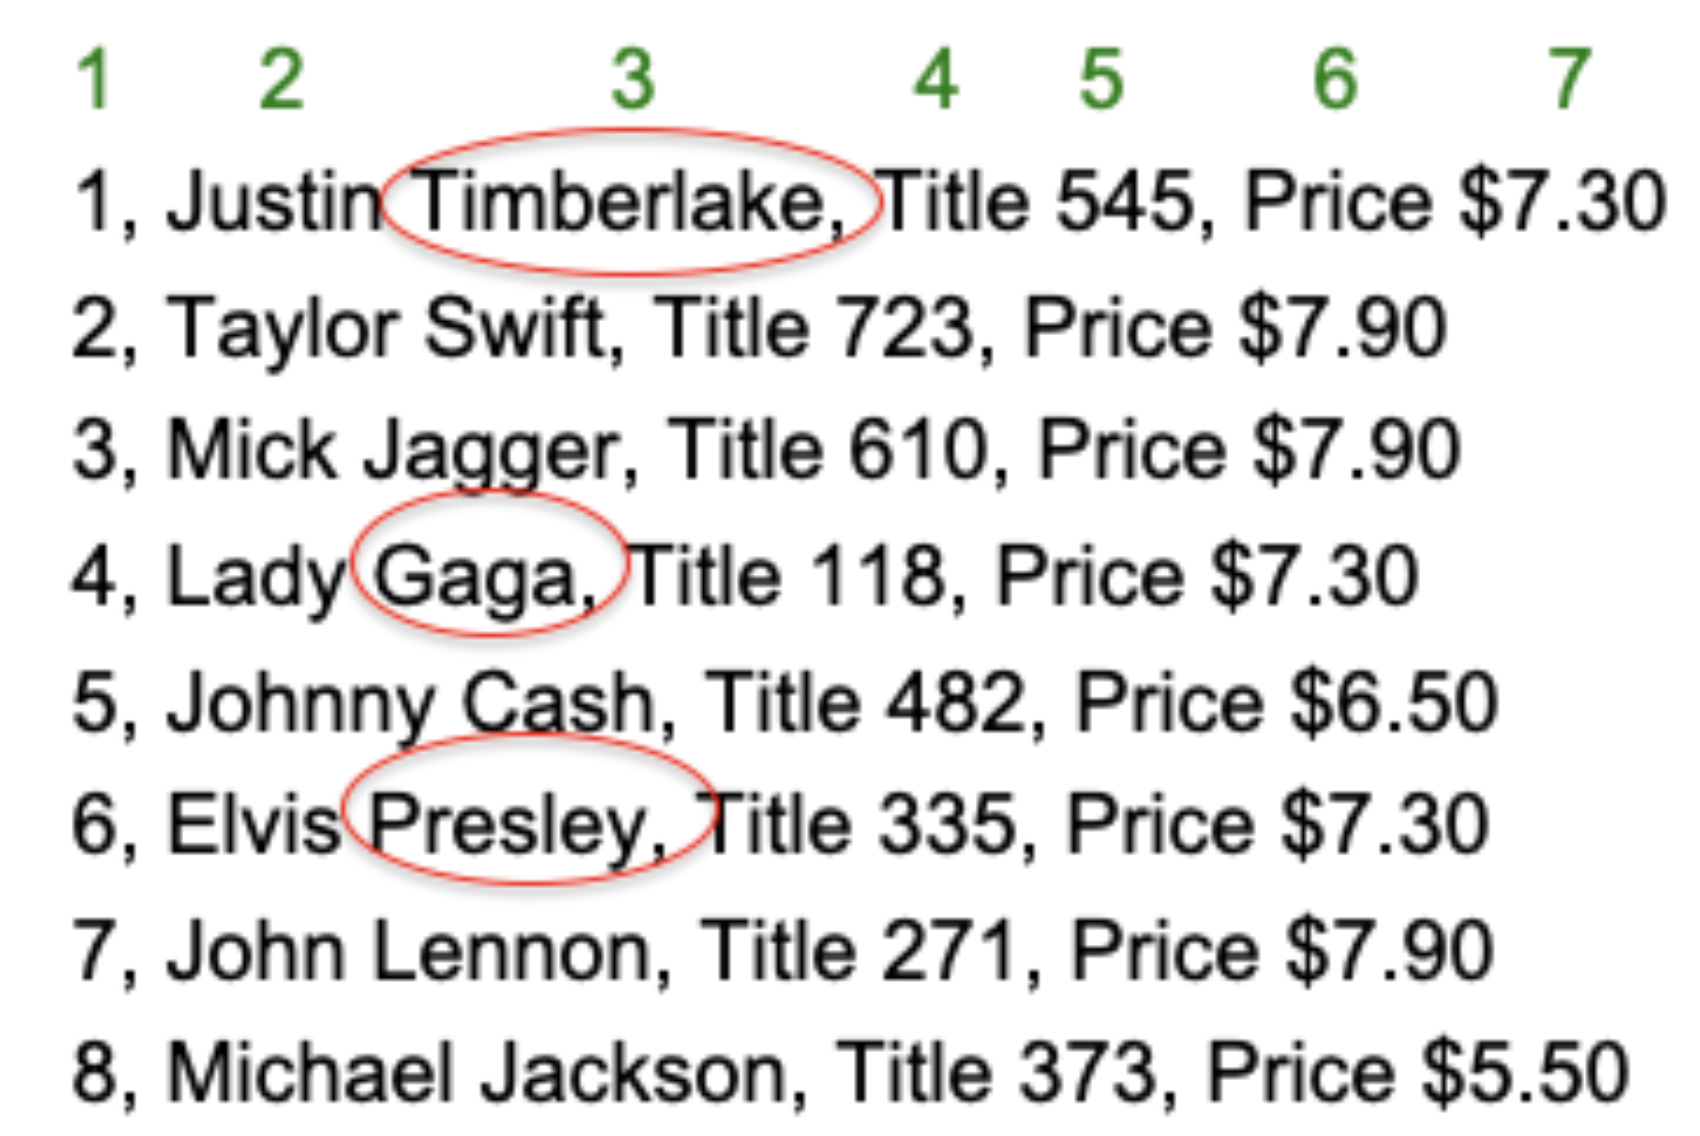
\includegraphics[width=0.6\textwidth,height=\textheight]{./Figures/awk.png}

\hypertarget{files-stream-editor-sed}{%
\subsection{\texorpdfstring{Files: \textbf{S}tream \textbf{ED}itor (sed)}{Files: Stream EDitor (sed)}}\label{files-stream-editor-sed}}

text substitution

\hypertarget{syntax-sed-spatternreplacement}{%
\subsubsection*{Syntax: sed s/pattern/replacement}\label{syntax-sed-spatternreplacement}}
\addcontentsline{toc}{subsubsection}{Syntax: sed s/pattern/replacement}

Examples:

\begin{verbatim}
echo "it’s a trap" | sed s/ra/ar/
\end{verbatim}

\begin{verbatim}
## it’s a tarp
\end{verbatim}

Say you want to change all price occurrences of \$7.90 to \$8.90 from table1.txt, and save the changes to a new file.

You can do this with sed.

\begin{verbatim}
sed 's/7.90/8.90/' table1.txt > table2.txt
\end{verbatim}

Use cat to display the contens of the new file:

\begin{verbatim}
cat table2.txt
\end{verbatim}

\begin{verbatim}
## 1, Justin Timberlake, Title 545, Price $7.30
## 2, Taylor Swift, Title 723, Price $8.90
## 3, Mick Jagger, Title 610, Price $8.90
## 4, Lady Gaga, Title 118, Price $7.30
## 5, Johnny Cash, Title 482, Price $6.50
## 6, Elvis Presley, Title 335, Price $7.30
## 7, John Lennon, Title 271, Price $8.90
## 8, Michael Jackson, Title 373, Price $5.50
\end{verbatim}

\hypertarget{the-bash-for-loop}{%
\subsection{The Bash ``for'' Loop}\label{the-bash-for-loop}}

Suppose we want to run a command for a \textbf{group of files} in a directory. We can use a for loop to target all of them at once.

\hypertarget{syntax-for-variablename-in-filenameexpression-do-command-variablename-done}{%
\subsubsection*{Syntax: for variablename in filenameexpression; do command \$\{variablename\}; done}\label{syntax-for-variablename-in-filenameexpression-do-command-variablename-done}}
\addcontentsline{toc}{subsubsection}{Syntax: for variablename in filenameexpression; do command \$\{variablename\}; done}

\begin{verbatim}
for file in *; do echo ${file}; done
\end{verbatim}

\begin{verbatim}
## covid.fasta
## newfile.txt
## SP1.fq
## table1.txt
## table2.txt
\end{verbatim}

\begin{itemize}
\tightlist
\item
  The part up to the first semicolon targets every file in the working directory with the ``*'' wildcard
\item
  The second part will sequentially echo each file in the working directory
\item
  The third part is required to terminate the loop
\end{itemize}

\hypertarget{help-with-command-syntax}{%
\subsection{Help with command syntax}\label{help-with-command-syntax}}

If you forget details of a certain command, documentation can easily be found with a web search.

There is also cheat sheet on the weebly site under Supplemental Documents.

\hypertarget{exercises}{%
\section{Exercises}\label{exercises}}

\begin{enumerate}
\def\labelenumi{\arabic{enumi}.}
\item
  Using awk, print to output the first names of artists with album prices over \$7.50 from ta- ble1.txt. Then redirect this output to a file named homework\_1.txt
\item
  Using sed, replace all commas with semicolons in table1.txt. Save this to a file named home- work\_2.txt
\item
  Piping history to grep, show all commands you've used with the expression ``ls''. Save this to a file named homework\_3.txt
\item
  Piping cat to wc -l on the history text file made during the tutorial, count the number of lines in it.
\item
  Using scp, download table1.txt to your own machine. Check it's there, then upload it back to logrus.
\end{enumerate}

\hypertarget{part-iii}{%
\section{PART III}\label{part-iii}}

\begin{enumerate}
\def\labelenumi{\arabic{enumi})}
\item
  Log on to logrus server
\item
  Enter the following command to log on to logrus:
\end{enumerate}

\begin{verbatim}
ssh -p 44111 username@gateway.training.ncgr.org
\end{verbatim}

\begin{itemize}
\tightlist
\item
  Don't forget to substitute \textbf{your} personal username in
\end{itemize}

\begin{enumerate}
\def\labelenumi{\arabic{enumi})}
\setcounter{enumi}{2}
\tightlist
\item
  Make a new directory under \textbf{your home directory}:
\end{enumerate}

\begin{verbatim}
mkdir fastq_files
\end{verbatim}

\begin{enumerate}
\def\labelenumi{\arabic{enumi})}
\setcounter{enumi}{3}
\tightlist
\item
  Enter into the new directory:
\end{enumerate}

\begin{verbatim}
cd fastq_files
\end{verbatim}

\begin{enumerate}
\def\labelenumi{\arabic{enumi})}
\setcounter{enumi}{4}
\tightlist
\item
  Move the fastq file from yesterday to the present working directory:
\end{enumerate}

\begin{verbatim}
mv ~/linuxc/SP1.fq .

ls -ltr
\end{verbatim}

\begin{verbatim}
## total 0
## lrwxrwxrwx 1 elavelle elavelle 28 Aug 17 22:50 SP1.fq -> /home/fds/unix_basics/SP1.f
\end{verbatim}

\begin{enumerate}
\def\labelenumi{\arabic{enumi})}
\setcounter{enumi}{5}
\tightlist
\item
  How can we count the number of records in a fastq file?
\end{enumerate}

\begin{verbatim}
grep -c "@cluster" SP1.fq
\end{verbatim}

\begin{verbatim}
## 250
\end{verbatim}

\begin{enumerate}
\def\labelenumi{\arabic{enumi})}
\setcounter{enumi}{6}
\tightlist
\item
  If you want to determine the number of lines in a file, you can use the ``wc'' command.
\end{enumerate}

\begin{verbatim}
cat SP1.fq | wc -l
\end{verbatim}

\begin{verbatim}
## 1000
\end{verbatim}

\begin{enumerate}
\def\labelenumi{\arabic{enumi})}
\setcounter{enumi}{7}
\tightlist
\item
  Why does the first command output 250 and the second 1000?
\end{enumerate}

\hypertarget{more-exercises}{%
\section{More Exercises}\label{more-exercises}}

\begin{enumerate}
\def\labelenumi{\arabic{enumi}.}
\item
  With one command, send a copy of table1.txt in the linuxc directory to your home directory with the name table1\_bu.txt
\item
  Print to standard output the last line of table1.txt
\item
  Use a loop to count the number of lines in all files in the linuxc directory.
\item
  Print to standard output the last names of music artists with album prices less than or equal to \$7.30
\item
  Create a file with only the accession numbers of the sequences contained in the covid.fasta file (with no additional spaces or symbols).
\end{enumerate}

\hypertarget{our-world-in-data}{%
\chapter{Our World in Data}\label{our-world-in-data}}

\hypertarget{practice-parsing}{%
\section{Practice parsing}\label{practice-parsing}}

Let's practice with a small file. Make sure you are in a \textbf{screen}.

\begin{enumerate}
\def\labelenumi{\arabic{enumi}.}
\item
  Make a directory under your home directory called ``parse''.
\item
  Go into that directory.
\item
  Copy the file ``pandemics.csv'' from this directory: ``/home/jm/linux\_practice/'' to the directory you just made.
\item
  Take a look at the file.
\item
  Sort by year an put it into a new file called ``sort.pandemic.csv''
  Note that you will need to change the delimiter to a comma (-t), tell it to sort numerically (-n), and tell it which column to sort (-k) sort -t, -n -k3 pandemics.csv \textgreater{} sort.pandemics.csv
\item
  Pull out all the instances that mention plague
  Note that grep is case sensitive by default so you might want to use the -i flag to make it case insensitive in case the is inconsistent
\item
  Pull out all the instance of the flu
\item
  Let's count the number of each type of pathogen (column 2). You could do this with a series of grep commands but with a big file you might not know all the possible pathogens and it would get tedious. So let's do this in a step-wise fashion and make sure each piece is as expected, then pipe it into the next step.\\
  a. First pull out column 2 using awk or cut\\
  b. Get the unique values (make sure you ``sort'' before you ``uniq'' or you will only deredundify adjacent identical values).\\
  c.~Get the count (hint: add -c to the uniq step)
\item
  Grab and count the organisms for the instances that mention plague
\end{enumerate}

Hint: It is the same as \#8 except you need to grab the plague lines first. When you put a command after the pipe it will read in the output of the previous command so only use the file name on the first command.

Click for All Answers

Note that there are often several ways to do things in linux and not all methods are shown.

\begin{verbatim}
1. mkdir ~/parse

2. cd ~/parse

3. cp /home/jm/linux_practice/pandemics.csv . [Don't forget the space and period at the end; the period says to name it the same thing.]

4. cat pandemics.csv [you could also use more, less, head, tail, or other commands]

5. sort -t, -nk 3 pandemics.csv > sort.pandemics.csv

6. grep -i plague sort.pandemics.csv

7. grep -i flu sort.pandemics.csv

8. awk -F, '{print $2}' sort.pandemics.csv | sort | uniq -c
     [Note that you can also use: "cut -d, -f2 pandemics.csv" for the first step]

9. grep -i plague sort.pandemics.csv | awk -F, '{print $2}' | sort | uniq -c
\end{verbatim}

\hypertarget{our-world-in-data-1}{%
\section{Our World in Data}\label{our-world-in-data-1}}

Now let's use the data from ``Our World In Data''. For things that are new, we have added some in-line answers but before you reveal the answer, try it yourself first using the hints provided.

\begin{enumerate}
\def\labelenumi{\arabic{enumi}.}
\setcounter{enumi}{9}
\item
  Copy the file ``owid-covid-data.csv'' from this directory: ``/home/jm/linux\_practice/'' to your ``parse'' directory.
\item
  Make sure you are in the ``parse'' directory.
\item
  How many rows are in the file? Use wc -l (wc = word count, -l = lines)
\end{enumerate}

Click for Answer

\begin{verbatim}
  wc -l owid-covid-data.csv
\end{verbatim}

\hfill\break

\begin{enumerate}
\def\labelenumi{\arabic{enumi}.}
\setcounter{enumi}{12}
\tightlist
\item
  How many columns? There is a special variable, NF, in awk, which prints the number of fields
\end{enumerate}

Note: this will print the number of fields in each row. You can hit ctrl-c if you don't want to go through the whole file

Click for Answer

\begin{verbatim}
  awk -F, '{print NF}' owid-covid-data.csv
\end{verbatim}

\hfill\break

\begin{enumerate}
\def\labelenumi{\arabic{enumi}.}
\setcounter{enumi}{13}
\tightlist
\item
  Let's look at hospital\_beds\_per\_thousand (column 60). We also need to get the location (country) from column 3 and the date from column 4. We'll pipe it into less so that we can scroll through it (to get out of less, hit ``q'').
\end{enumerate}

Click for Answer

\begin{verbatim}
  cut -d, -f 3,4,60 owid-covid-data.csv | less
\end{verbatim}

\hfill\break

\begin{enumerate}
\def\labelenumi{\arabic{enumi}.}
\setcounter{enumi}{14}
\item
  There are lots of dates for each country. Let's limit it to early in the pandemic (2020-01-03), which is the first available date. Put it into a file called ``beds.2020-01-03.csv'' so we don't have to keep generating it.
\item
  What country had the least beds per thousand on 2020-01-03 and which has the most? Hint: Sort by the number of beds and pipe it into less.
\end{enumerate}

Note: Some lines have missing data and will sort at the top of the file so you will have to scroll down.

\begin{enumerate}
\def\labelenumi{\arabic{enumi}.}
\setcounter{enumi}{16}
\tightlist
\item
  How many beds were there in the United States on 2020-01-03?
\end{enumerate}

Hint: There is a ``United States'' and a ``United States Virgin Islands''. To avoid getting the latter, have the match end with a comma. Also, require grep to start the match at the beginning of the line (\^{}). It is good practice to be specific when using grep.

Click for Answer

\begin{verbatim}
  grep "^United States," beds.2020-01-03.csv
\end{verbatim}

\hfill\break

\begin{enumerate}
\def\labelenumi{\arabic{enumi}.}
\setcounter{enumi}{17}
\tightlist
\item
  How many beds were there in your three countries on 2020-01-03?
\end{enumerate}

If your countries don't have data on that date, go back to the original file and see if you can find data for any date.

Hint: we'll use the extended version of grep which will allow us to search all 3 at once. Use the -E flag and put the things you are searching for in double quotes, seperated by pipes.

Click for Answer

\begin{verbatim}
  grep -E "^Sweden,|^Norway,|^Denmark," beds.2020-01-03.csv
\end{verbatim}

\hfill\break

\begin{enumerate}
\def\labelenumi{\arabic{enumi}.}
\setcounter{enumi}{18}
\item
  Create a file that has only the United States data for beds with the same three columns we have been using. Call it usbeds.csv. We'll use this file for the questions below.
\item
  Get the number of beds in the United States for each day in 2020.
\item
  Get the number of beds in the United States for the first COVID wave (March through September 2020).
\end{enumerate}

Hint: Use sed to remove the dashes then awk with \$2\textgreater=20200301\&\&\$2\textless=20200930.

Click for Answer

sed `s/-//g' usbeds.csv \textbar{} awk `\$2\textgreater=20200301\&\&\$2\textless=20200930\{print\}'

\hfill\break

\begin{enumerate}
\def\labelenumi{\arabic{enumi}.}
\setcounter{enumi}{21}
\tightlist
\item
  BONUS: Get the average number of beds in the United States for the first COVID wave (March through September 2020). This is a tough one. See if you can understand the code.
\end{enumerate}

Click for Answer

sed `s/-//g' usbeds.csv \textbar{} sed `s/-//g' \textbar awk -F, `\$2\textgreater=20200301\&\&\$2\textless=20200930\{SUM+=\$3;CNT+=1\}END\{print SUM/CNT\}'

\hfill\break

Click for All Answers

\begin{verbatim}
10. cp /home/jm/linux_practice/owid-covid-data.csv . 

11. pwd [If you aren't in that directory you can: "cd ~/parse"]

12. wc -l owid-covid-data.csv

13. awk -F, '{print NF}' owid-covid-data.csv

14. cut -d, -f 3,4,60 owid-covid-data.csv | less

15. cut -d, -f 3,4,60 owid-covid-data.csv | grep 2020-01-03 > beds.2020-01-03.csv

16. sort -t, -n -k3 beds.2020-01-03.csv | less

    Least: Mali,2020-01-03,0.1
    
    Most: Monaco,2020-01-03,13.8

17. grep "^United States," beds.2020-01-03.csv

18. grep -E "^Sweden,|^Norway,|^Denmark," beds.2020-01-03.csv

19. cut -d, -f 3,4,60 owid-covid-data.csv | grep "^United States," > usbeds.csv

20. grep 2020 usbeds.csv

21. sed 's/-//g' usbeds.csv | sed 's/-//g' |awk -F, '$2>=20200301&&$2<=20200930{print}'

22. sed 's/-//g' usbeds.csv | sed 's/-//g' |awk -F, '$2>=20200301&&$2<=20200930{SUM+=$3;CNT+=1}END{print SUM/CNT}'

\end{verbatim}

\hypertarget{practice-with-your-3-countries}{%
\section{Practice with your 3 countries}\label{practice-with-your-3-countries}}

Now practice on your own. Choose another variable and see if there are any interesting differences between your 3 countries. Explore at least 3 other variables.

Hint: You can look at the variables by heading the first line of the file.

\begin{verbatim}
    head -1 owid-covid-data.csv
\end{verbatim}

Hint: If you prefer to have them each on their own line you can use sed to replace the commas with hard returns. Make sure to use the global ``g'' at the end so that every comma is replaced and not just the first one on each line.

\begin{verbatim}
    head -1 owid-covid-data.csv | sed 's/,/\n/g'
\end{verbatim}

Hint: awk will also print out the row number for you (which corresponds to the column number for that variable in the original file). The NR variable is a special awk variable that will print the row.

\begin{verbatim}
    head -1 owid-covid-data.csv | sed 's/,/\n/g' |awk '{print NR "\t" $1}'
\end{verbatim}

\hypertarget{ncbi-sars-cov-2-genome-sequences}{%
\chapter{NCBI SARS-CoV-2 Genome Sequences}\label{ncbi-sars-cov-2-genome-sequences}}

\hypertarget{getting-sequences-from-ncbi}{%
\section{Getting Sequences from NCBI}\label{getting-sequences-from-ncbi}}

See pdf.

\hypertarget{exploring-sequence-files}{%
\section{Exploring Sequence Files}\label{exploring-sequence-files}}

Let's start with the Denmark, Norway, Sweden files. Make sure you are in the NCBIdata directory.

\begin{enumerate}
\def\labelenumi{\arabic{enumi}.}
\item
  Grab just the sequence header lines.
\item
  How many sequences are there for Denmark?
\item
  Grab just the country out of the fasta headers
\end{enumerate}

Your headers should have these fields, delimitted by a pipe (make sure you put the pipes in quotes so it doesn't interpret it):

\begin{verbatim}
  1) Accession
  2) Genbank Title
  3) Collection Date
  4) Country
  5) GEO Location
  6) Length
  7) Pangolin (variant)
  8) SRA Accession
  9) Sequence Type
\end{verbatim}

\begin{enumerate}
\def\labelenumi{\arabic{enumi}.}
\setcounter{enumi}{3}
\tightlist
\item
  How many sequences are there for each country?
\end{enumerate}

Hint: Use sort then uniq -c (the latter gets counts of all the unique values).

\begin{enumerate}
\def\labelenumi{\arabic{enumi}.}
\setcounter{enumi}{4}
\item
  How many sequences are there for each Geo Location? Some will just have the country there but others will have more granular information.
\item
  How many sequences are there for each pangolin variant? What is the dominant one? Look up more information for the dominant lineage at this site: \url{https://cov-lineages.org/lineage_list.html}
\item
  Haw many sequences are there for each pangolin variant in each country?
\item
  How many sequences are not blank in the collection data field?
\end{enumerate}

\begin{verbatim}
Hint: Use "^$" in grep to find lines that have nothing between the start "^" and end "$" of the line.
\end{verbatim}

\begin{enumerate}
\def\labelenumi{\arabic{enumi}.}
\setcounter{enumi}{8}
\tightlist
\item
  What is the first and last date in your sequence file?
\end{enumerate}

Hint: There are lots of different ways to do this, some of which involve more scrolling than others. Here is one strategy that just gets the earliest and latest dates. Do each step and check it then pipe it into the next step.

\begin{verbatim}
  1) Get the header lines
  2) Grab the collection data column (#3)
  3) Remove blanks
  4) Sort numerically: sort -n
  5) grab the first and last lines--you need the parentheses: (head -1; tail -1)
\end{verbatim}

\begin{enumerate}
\def\labelenumi{\arabic{enumi}.}
\setcounter{enumi}{9}
\tightlist
\item
  Find the first and last collection date in your sequence file for each country. Try to use a for loop. Since we haven't used these much I'll put an answer here for you.
\end{enumerate}

Note: for some reason, the (head -1; tail -1) trick doesn't seem to work inside a for loop. So, do the earliest date first. Then use the up arrow to get the command back and alter it for the latest date.

Click for Answer

\begin{verbatim}
    for i in 'Denmark' 'Norway' 'Sweden'; do
      echo $i
      grep $i sequences.fasta | cut -f 3 -d '|' | grep -v "^$" | sort -n | head -1
  done
\end{verbatim}

\hfill\break

Click for All Answers

Note that there are often several ways to do things in linux and not all methods are shown.

\begin{verbatim}
1. grep '>' sequences.fasta

2. grep -c 'Denmark' sequences.fasta

14 sequences for Denmark

3. grep '>' sequences.fasta | cut -f 4 -d '|'

4. grep '>' sequences.fasta | cut -f 4 -d '|' | sort |uniq -c

     14 Denmark
     
      5 Norway
      
    616 Sweden

5. grep '>' sequences.fasta | cut -f 5 -d '|' | sort |uniq -c

     14 Denmark
     
      2 Norway
      
      3 Norway: Bergen
      
    566 Sweden
    
      1 Sweden:Goteborg
      
     44 Sweden: Orebro
     
      5 Sweden:Stockholm, Sweden

6. grep '>' sequences.fasta | cut -f 7 -d '|' | sort |uniq -c

The dominant pangolin variant is B.1 which occurs 429 times.

7. grep '>' sequences.fasta | cut -f 4,7 -d '|' | sort |uniq -c

8. grep '>' sequences.fasta | cut -f 3 -d '|' |grep -c "^$"

9. grep '>' sequences.fasta | cut -f 3 -d '|' | grep -v "^$" | sort -n | (head -1; tail -1)

10. The first is for the earliest date and the second for the latest date.

for i in 'Denmark' 'Norway' 'Sweden'; do
  echo $i
  grep $i sequences.fasta | cut -f 3 -d '|' | grep -v "^$" | sort -n | head -1
done

for i in 'Denmark' 'Norway' 'Sweden'; do
  echo $i
  grep $i sequences.fasta | cut -f 3 -d '|' | grep -v "^$" | sort -n | tail -1
done
\end{verbatim}

\hypertarget{practice-with-your-3-countries-1}{%
\section{Practice with your 3 countries}\label{practice-with-your-3-countries-1}}

Run through these exercises again with your 3 countries and record the answers in your project powerpoint or elsewhere. We'll talk about what you found.

\hypertarget{plotting}{%
\section{Plotting}\label{plotting}}

We'll plot some of the information about our sequences using R on the command line and the ggplot2 library. Get into a screen if you aren't already in one (screen -dr will reconnect you to a previous screen). Navigate to your NCBIdata directory.

\hypertarget{r}{%
\section{R}\label{r}}

The R Project for Statistical Computing

\url{https://www.r-project.org/}

R studio (Integrated Development Environment)

\url{https://posit.co/download/rstudio-desktop/}

\hypertarget{ggplot2}{%
\section{ggplot2}\label{ggplot2}}

Handy gglot2 references:

ggplot2 gallery

\url{http://www.r-graph-gallery.com/portfolio/ggplot2-package/}

ggplot2 cheatsheets

\url{http://ggplot2.tidyverse.org/reference/}

ggplot2 documentation

\url{https://cran.r-project.org/web/packages/ggplot2/ggplot2.pdf}

\hfill\break

\begin{enumerate}
\def\labelenumi{\arabic{enumi}.}
\setcounter{enumi}{10}
\tightlist
\item
  Make a tab-delimitted text file with the information from your sequence headers.
\end{enumerate}

\begin{verbatim}
1) Grab the sequence headers
2) Remove the greater than sign at the beginning of the header line
3) Replace the pipes with tabs (Hint: In sed use \t to represent a tab)
4) Make the date numeric by replacing the dashes. The sed command below will allow you to replace dashes only in the date.

If you are interested in understanding the sed command: It looks for one or more (+) numbers ([0-9]) then a dash, more numbers, a dash and more numbers. The parentheses capture the sets of numbers so that it can return them as \1 for the first set, \2 for the second set, and \3 for the third set.

sed -E 's/([0-9]+)-([0-9]+)-([0-9]+)/\1\2\3/'
5) Put it into a file called Denmark_Norway_Sweden_seq_info.txt
\end{verbatim}

The R environment on logrus needs to be activated (note that on some systems it is installed differently and you don't need to activate).

\begin{verbatim}
conda activate visualization
\end{verbatim}

Open up R.

\begin{verbatim}
R
\end{verbatim}

Now we are in R. The R command line is similar to linux but the commands are a little bit different as you will notice as we walk through it. Note that you can use the up arrow to get back previous commands as in linux. ctrl-c works the same as well.

Load the ggplot2 library.

\begin{verbatim}
library(ggplot2)
\end{verbatim}

See what your working directory is (it should be the directory you were in when you entered R). Note that you can change your working directory with the setwd() command, putting the path to the new directory in the parentheses.

\begin{verbatim}
getwd()
\end{verbatim}

Let's read in the tab-delimitted file we created. We'll use the read.table command. To find out more, let's look at the help for that command using a question mark before the command (equivalent to the man command in linux).

\begin{verbatim}
?read.table
\end{verbatim}

It prints out a lot of documentation including commands that are similar. The first part is below. The help documentation describes the command and gives you all the arguments you can use along with their defaults. Arguments go in the parentheses. Some are required but others are optional.

\begin{enumerate}
\def\labelenumi{\arabic{enumi}.}
\setcounter{enumi}{11}
\item
  The two arguments that I use the most are ``header'' and ``sep''. Look at the usage section of the help below or in your terminal. What are the defaults for these two arguments?
\item
  Scroll down in the help (the up and down arrows go up or down line by line; the space bar jumps you down a page at a time) to the arguments section. Read about header and sep. What do these arguments do? What do the defaults mean?
\end{enumerate}

Note: To get out of help, hit ``q''.

Read in our data file and put it into a variable. We'll name our variable dns for Denmark, Norway, Sweden.

\begin{verbatim}
dns = read.table("Denmark_Norway_Sweden_seq_info.txt", header=FALSE, sep="\t")
\end{verbatim}

Let's take a look at the variable with our data The head command in R has 6 rows by default and it wraps lines as a group if they are too long for the screen.

\begin{verbatim}
head(dns)
\end{verbatim}

\begin{enumerate}
\def\labelenumi{\arabic{enumi}.}
\setcounter{enumi}{13}
\item
  Take a look at the help for the head command and see if you can figure out how to show 10 lines.
\item
  How do you think you could look at the end of the dns variable?
\end{enumerate}

When you look at the dns variable, it shows column and row names. Since we didn't have a header line in our tab-delimitted file, it just defaults to V1, V2 (V stands for vector). Since we didn't have row names, it defaults to numbers. Let's fix the column names. The ``c'' concatenates a list of things together to be fed in as a group.

\begin{verbatim}
colnames(dns) = c("Accession", "Genbank_Title", "Collection_Date", "Country", "GEO_Location", "Length", "Pangolin_Variant", "SRA_Accession", "Sequence_Type")
\end{verbatim}

Then check it with the head command.

\begin{verbatim}
    Accession
1 OR079912.1
2 OQ843561.1
3 OQ816151.1
4 OQ816152.1
5 OQ816154.1
6 OQ816156.1
                                                                                                           Genbank Title
1                  Severe acute respiratory syndrome coronavirus 2 isolate SARS-CoV-2/human/NOR/P9/2020, complete genome
2             Severe acute respiratory syndrome coronavirus 2 isolate SARS-CoV-2/human/DNK/DK-AHH8/2022, complete genome
3 Severe acute respiratory syndrome coronavirus 2 isolate SARS-CoV-2/human/SWE/01_SE100_21CS503718/2020, complete genome
4 Severe acute respiratory syndrome coronavirus 2 isolate SARS-CoV-2/human/SWE/01_SE100_21CS504474/2020, complete genome
5 Severe acute respiratory syndrome coronavirus 2 isolate SARS-CoV-2/human/SWE/01_SE100_21CS503085/2020, complete genome
6 Severe acute respiratory syndrome coronavirus 2 isolate SARS-CoV-2/human/SWE/01_SE100_21CS502014/2020, complete genome
  Collection Date Country GEO Location Length Pangolin Variant SRA Accession
1      2020-10-14  Norway       Norway  29825          B.1.258
2      2022-12-01 Denmark      Denmark  29752        BQ.1.1.20
3      2020-03-03  Sweden       Sweden  29736              B.1
4      2020-03-10  Sweden       Sweden  29736              B.1
5      2020-03-11  Sweden       Sweden  29736              B.1
6      2020-03-13  Sweden       Sweden  29736              B.1
  Sequence Type
1       GenBank
2       GenBank
3       GenBank
4       GenBank
5       GenBank
6       GenBank
\end{verbatim}

\hfill\break

The Collection Date wasn't recognized as numeric so let's fix that. The \$ after the dns refers to a column. We will just overwrite it in the same column.

\begin{verbatim}
dns$"Collection_Date" = as.numeric(dns$"Collection_Date")
\end{verbatim}

Time to plot!

The gglot2 library allows you to have a large amount of control over nearly all aspects of the plot. It also allows you to plot in layers, getting a base plot and then adding colors, lines, text, etc on top of it. It is part of the tidyverse universe and uses a Layered Grammar of Graphics (\url{https://towardsdatascience.com/a-comprehensive-guide-to-the-grammar-of-graphics-for-effective-visualization-of-multi-dimensional-1f92b4ed4149} and \url{https://www.jstor.org/stable/pdf/25651297.pdf?casa_token=KAMBWbsPZdwAAAAA:VHQTVEC762l7U6s6GWzRlYJNz5JaqfduQy1S04_LF6f3PUZjAh71Bva7WEIpROPBUx2BF9GL5bM0HOtDH_Zft81ycAcJ0971YeHDfrfHKBrgyw6G6fAG}) to concisely describe graphical components that are shared across different graphs. In other words, it gives you tools to add and manipulate specific pieces of graphical output.

We will put each plot into a png file. Note that we can also put it into a pdf file by changing the code below to pdf. The pdf has the advantage of being able to put in multiple plots on separate pages. After plotting we need to use dev.off() so that R closes the file it is printing to.

\hypertarget{histogram-of-collection-dates}{%
\subsection{Histogram of Collection Dates}\label{histogram-of-collection-dates}}

\begin{verbatim}
png("dates_histogram.png")

ggplot(dns, aes(x=Collection_Date)) + geom_histogram()

dev.off()
\end{verbatim}

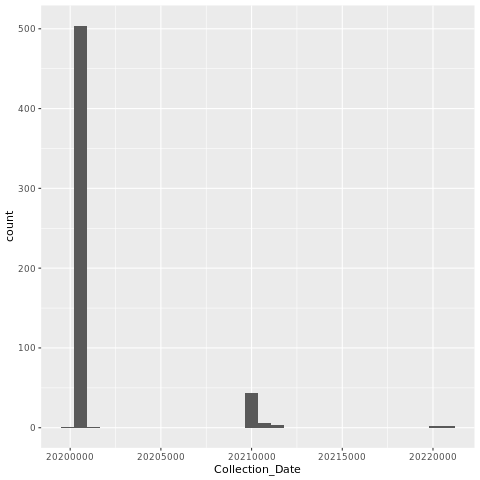
\includegraphics[width=0.5\textwidth,height=\textheight]{./Figures/dates_histogram.png}

\hypertarget{plot-length-x-variants}{%
\subsection{Plot Length x Variants}\label{plot-length-x-variants}}

Let's plot the genome length by the variant to see if there are any patterns. Some variants have insertions or deletions compared to others, for instance. On the other hand, not all genome assemblies make it to the ends of the viral RNA genome so this will add some noise.

We'll use a scatter plot. First we identify the data frame (dns) that we want to use. Then we assign fields to the x and y axis. After that we'll add the scatter plot layer (geom\_point). We'll add another layer to limit the x axis.

\begin{verbatim}
png("lengthxvariants.png")

ggplot(dns, aes(x=Length,y=Pangolin_Variant)) + geom_point() + xlim(29500,30000)

dev.off()
\end{verbatim}

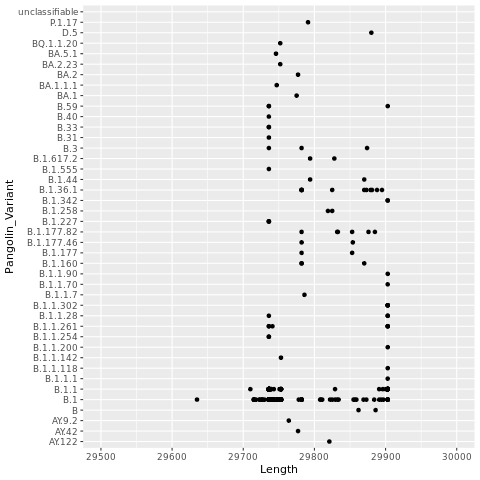
\includegraphics[width=0.5\textwidth,height=\textheight]{./Figures/lengthxvariants.png}

Now, let's color the points by Country.

\begin{verbatim}
png("lengthxvariants.color.png")

ggplot(dns, aes(x=Length,y=Pangolin_Variant,color=Country)) + geom_point() + xlim(29500,30000)

dev.off()
\end{verbatim}

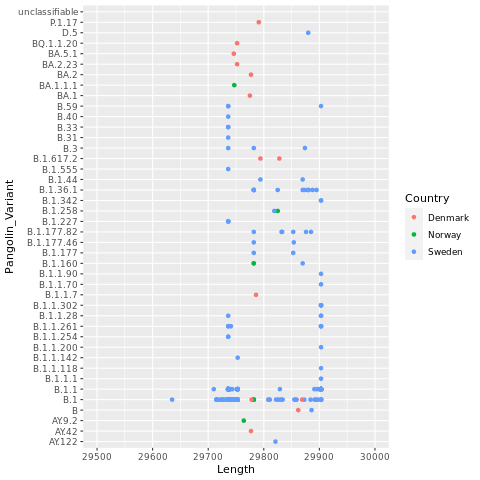
\includegraphics[width=0.5\textwidth,height=\textheight]{./Figures/lengthxvariants.color.png}

\hypertarget{plot-collection-date-x-variants}{%
\subsection{Plot Collection Date x Variants}\label{plot-collection-date-x-variants}}

\begin{enumerate}
\def\labelenumi{\arabic{enumi}.}
\setcounter{enumi}{15}
\tightlist
\item
  Now try to plot the collection date (x axis) by the variants (y axis), coloring by the country.
\end{enumerate}

\hypertarget{plot-collection-date-x-variants-for-your-3-countries}{%
\subsection{Plot Collection Date x Variants for your 3 countries}\label{plot-collection-date-x-variants-for-your-3-countries}}

Now make a plot of Collection Date x Variants for your 3 countries and add it to your powerpoint.

Go to \url{https://covariants.org/} to scroll down to the table and the phylogenetic tree to put some context around the variants.

At that same site, explore the ``per country'' and ``cases'' buttons for your 3 countries. Note that the graphs are interactive so you can hover over specific dates where you might have a lot of NCBI genome sequences. Grab screenshots to put into your powerpoint (be sure to record the date you grabbed the screenshot on the slide). How representative are the NCBI genome sequences?

Note: we'll be getting sequences from another source as well so don't worry if they aren't too representative.

Click for All Answers

\begin{verbatim}
11. grep '>' sequences.fasta | sed 's/>//'|sed 's/|/\t/g'|sed -E 's/([0-9]+)-([0-9]+)-([0-9]+)/\1\2\3/' > Denmark_Norway_Sweden_seq_info.txt

12. header = FALSE and sep = ""

13. The header arguement determines whether you have a header line in your file with the names of variables.

While the header default is false, if you don't explicitly put in header=FALSE, it might decide that there is a header line if the first row has one fewer field than the rest. I like to explicitly tell read.table whether there is a header row or not.

The sep variable determines the field separator character.

The sep default is blank ("") and means white space. In other words, read.table will split the file up on one or more spaces, tabs, etc. With tab-delimitted files, you don't normally have to specify the tab variable but since we also have spaces in some of our fields, if we keep sep as whitespace, it will separate on all the spaces as well. So we will need to specify it.

14. head(dns, n=10) or head(dns, n=10L)

15. tail(dns)

16.

png("datexvariants.color.png")

ggplot(dns, aes(x=Collection_Date,y=Pangolin_Variant,color=Country)) + geom_point()

dev.off()
\end{verbatim}

\hypertarget{gisaid-sars-cov-2-genome-sequences}{%
\chapter{GISAID SARS-CoV-2 Genome Sequences}\label{gisaid-sars-cov-2-genome-sequences}}

\hypertarget{gisaid}{%
\section{GISAID}\label{gisaid}}

\begin{figure}
\centering
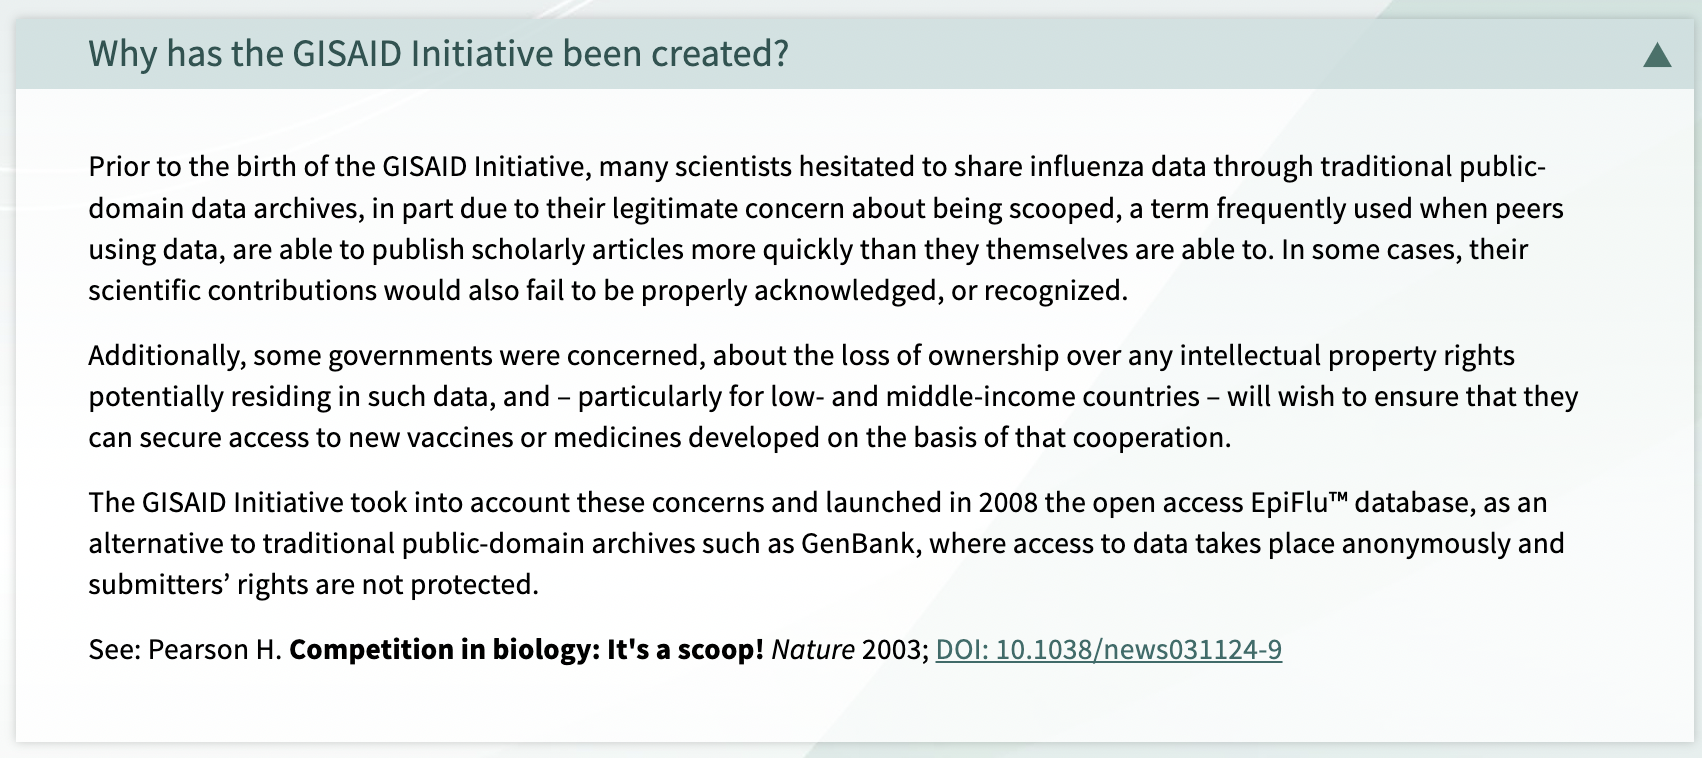
\includegraphics[width=0.5\textwidth,height=\textheight]{./Figures/gisaid.png}
\caption{GISAID}
\end{figure}

If you haven't already, please sign up for a GISAID account. The account is required to access sequences, though first we will explore one of their web tools in detail.

\hypertarget{phylodynamics}{%
\section{Phylodynamics}\label{phylodynamics}}

Click on hCoV-19 in the Phylodynamics section.

Note that if you logged in it will push you over to epicov.org. You might need to go back to gisaid.org.

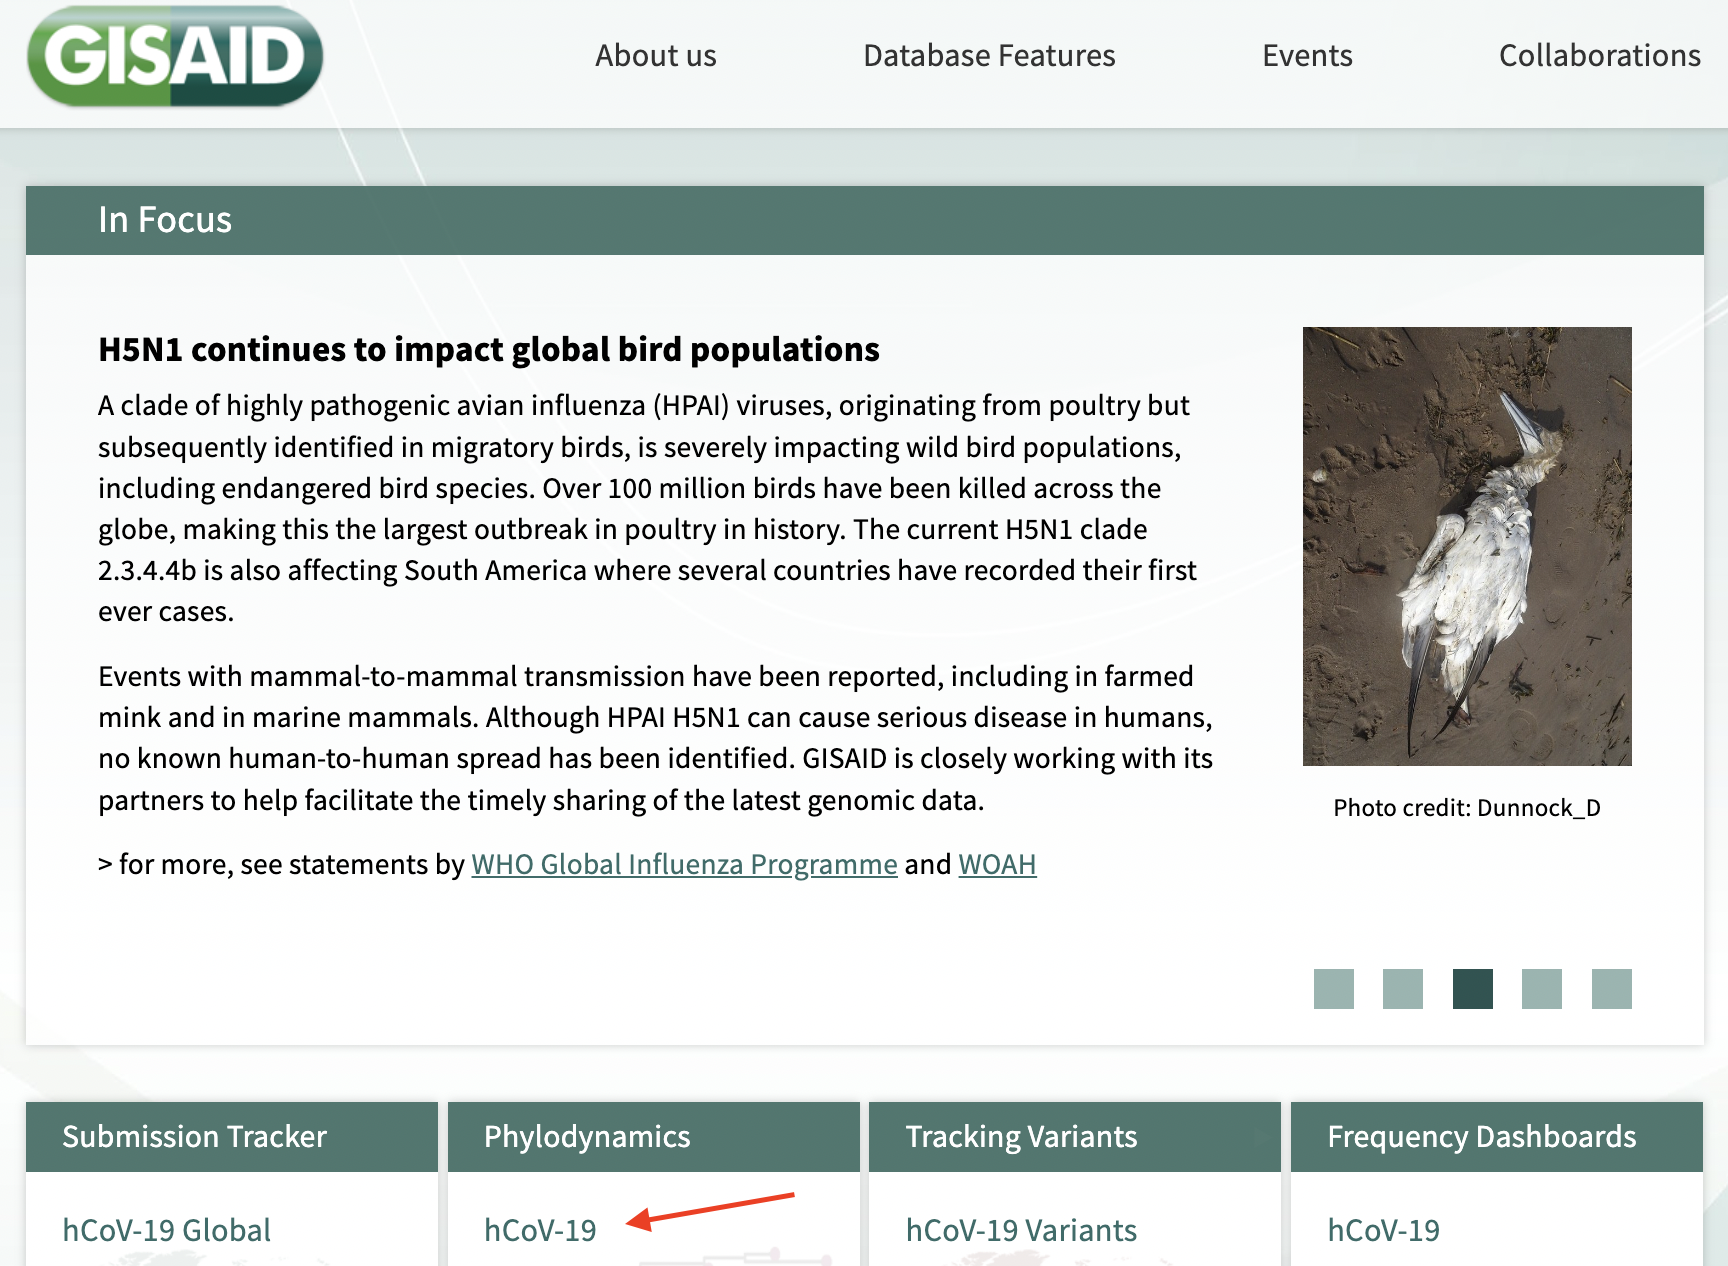
\includegraphics[width=0.5\textwidth,height=\textheight]{./Figures/Phylodynamics.png}

Follow along with one or more of your 3 countries (and get screenshots marked with today's dates into your slides). If none of your 3 countries are availble, choose another country to follow along with for now. I'll be using Denmark (Norway and Sweden are not available).

We can create a transmission map color-coded by time.

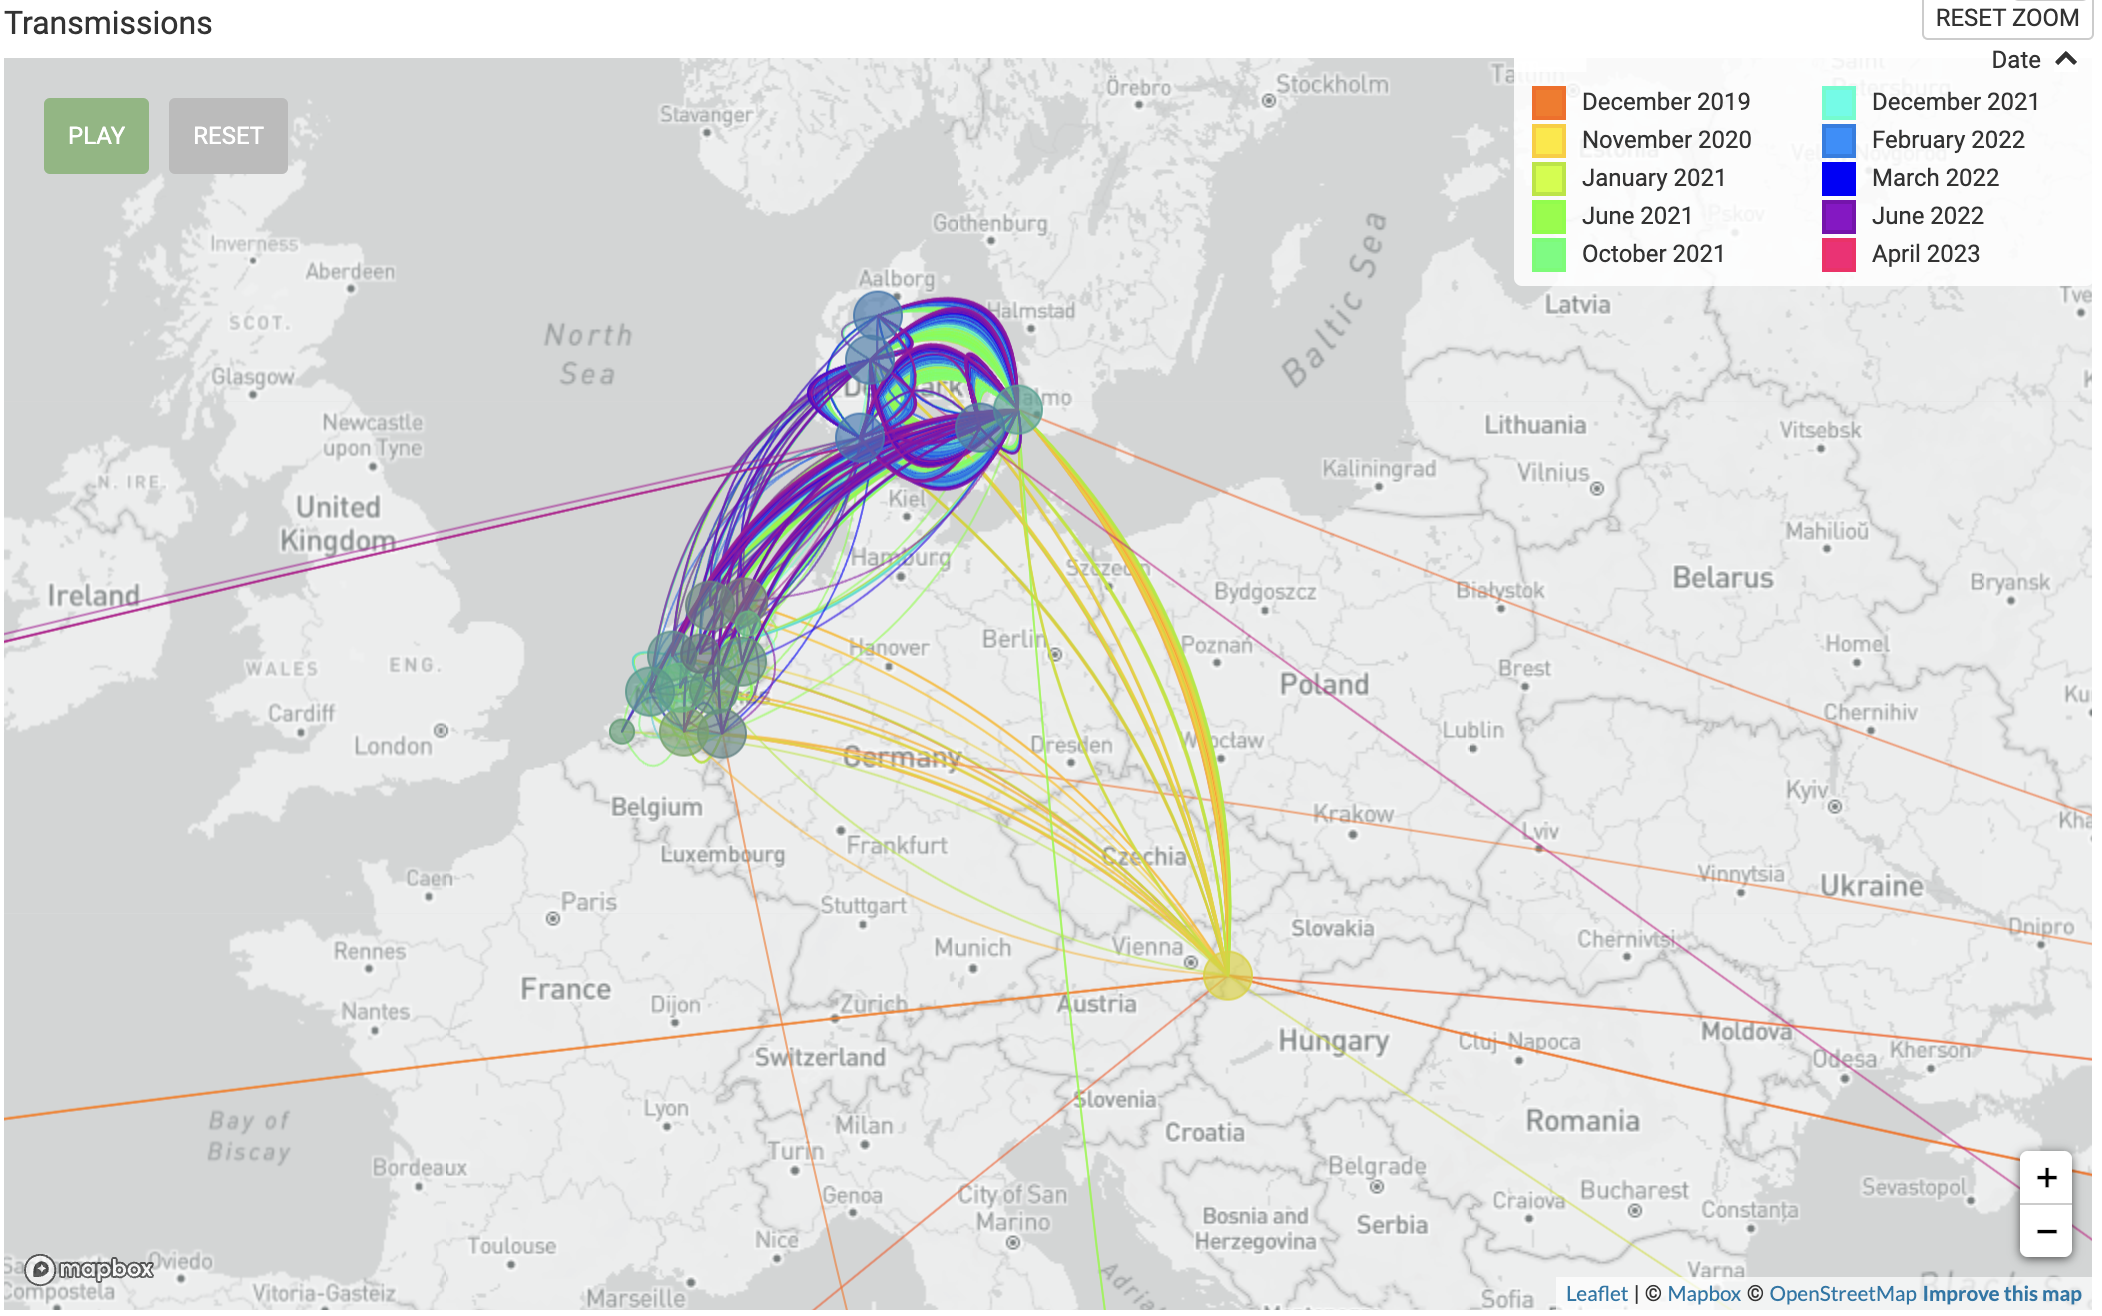
\includegraphics[width=0.5\textwidth,height=\textheight]{./Figures/DenmarkTransmission.png}

What do you learn from the Denmark graph?

Click for Possible Answer

\begin{verbatim}
  Many of the earliest transmissions came from a region at the borders of Austria, Hungary, and Slovakia.
  
  Later on, there is a lot of transmission within the country and some also a lot of transmission routes between Denmark and the Netherlands.
  
  Note that the transmission data might be affected by which countries have the most data available.
\end{verbatim}

\hfill\break

We can look at a tree (scroll down) of the different named variants either by time or by divergence. For the divergence, I also added amino acid changes. We talk about subvariants of omicron but notice that there is a lot of genetic variation within each variant. Even two different genomes that are both from the same subvariants of omicron may not be identical, though they will both have the variants that define that subvariant.

\begin{figure}
\centering
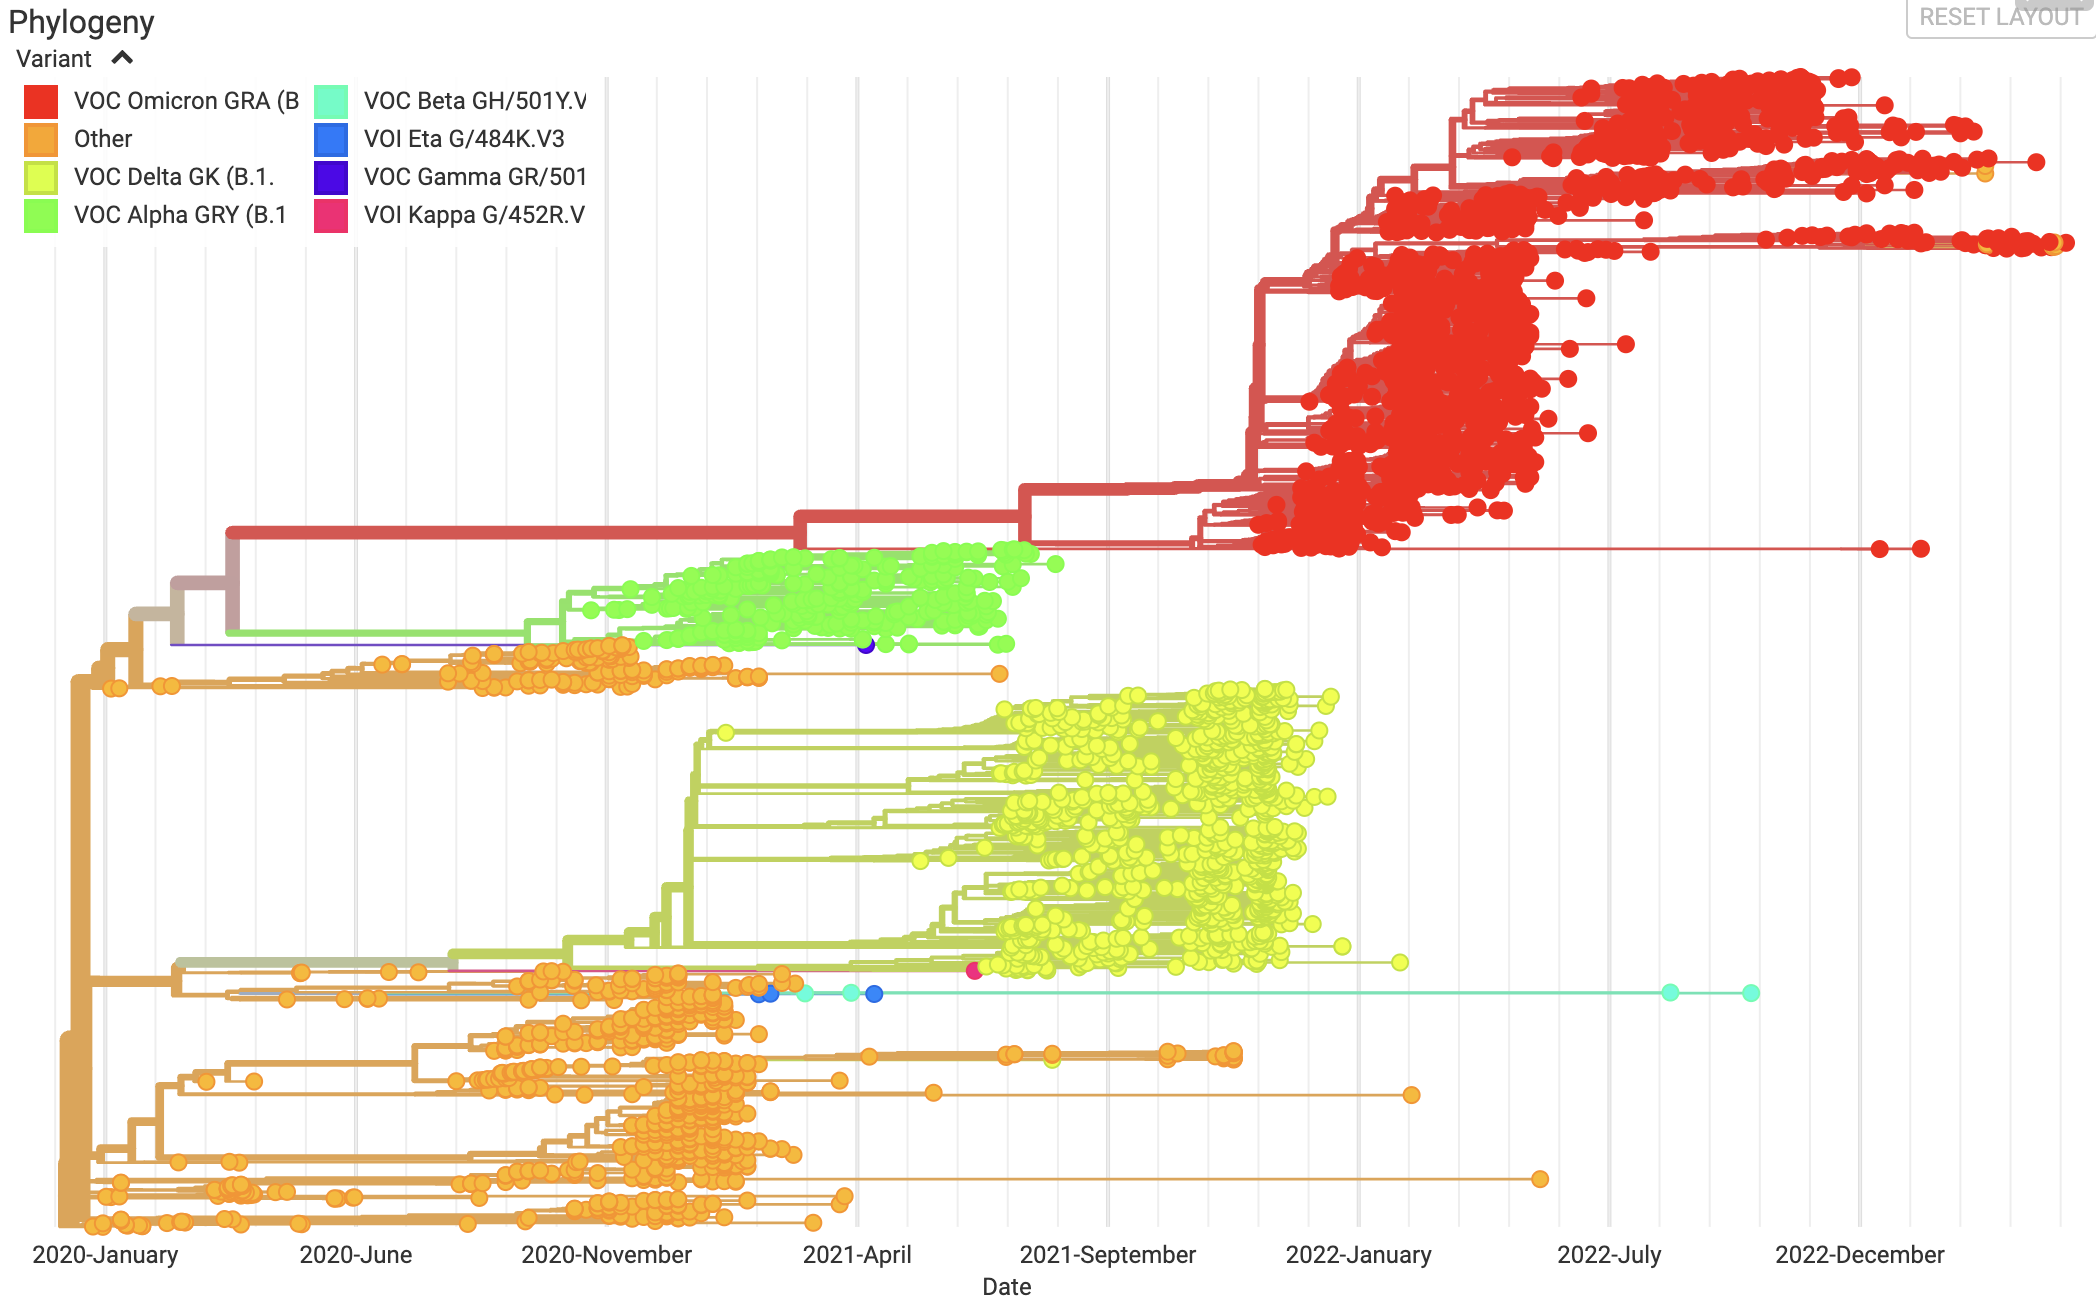
\includegraphics[width=0.7\textwidth,height=\textheight]{./Figures/DenmarkRectangularTime.png}
\caption{Time}
\end{figure}

\begin{figure}
\centering
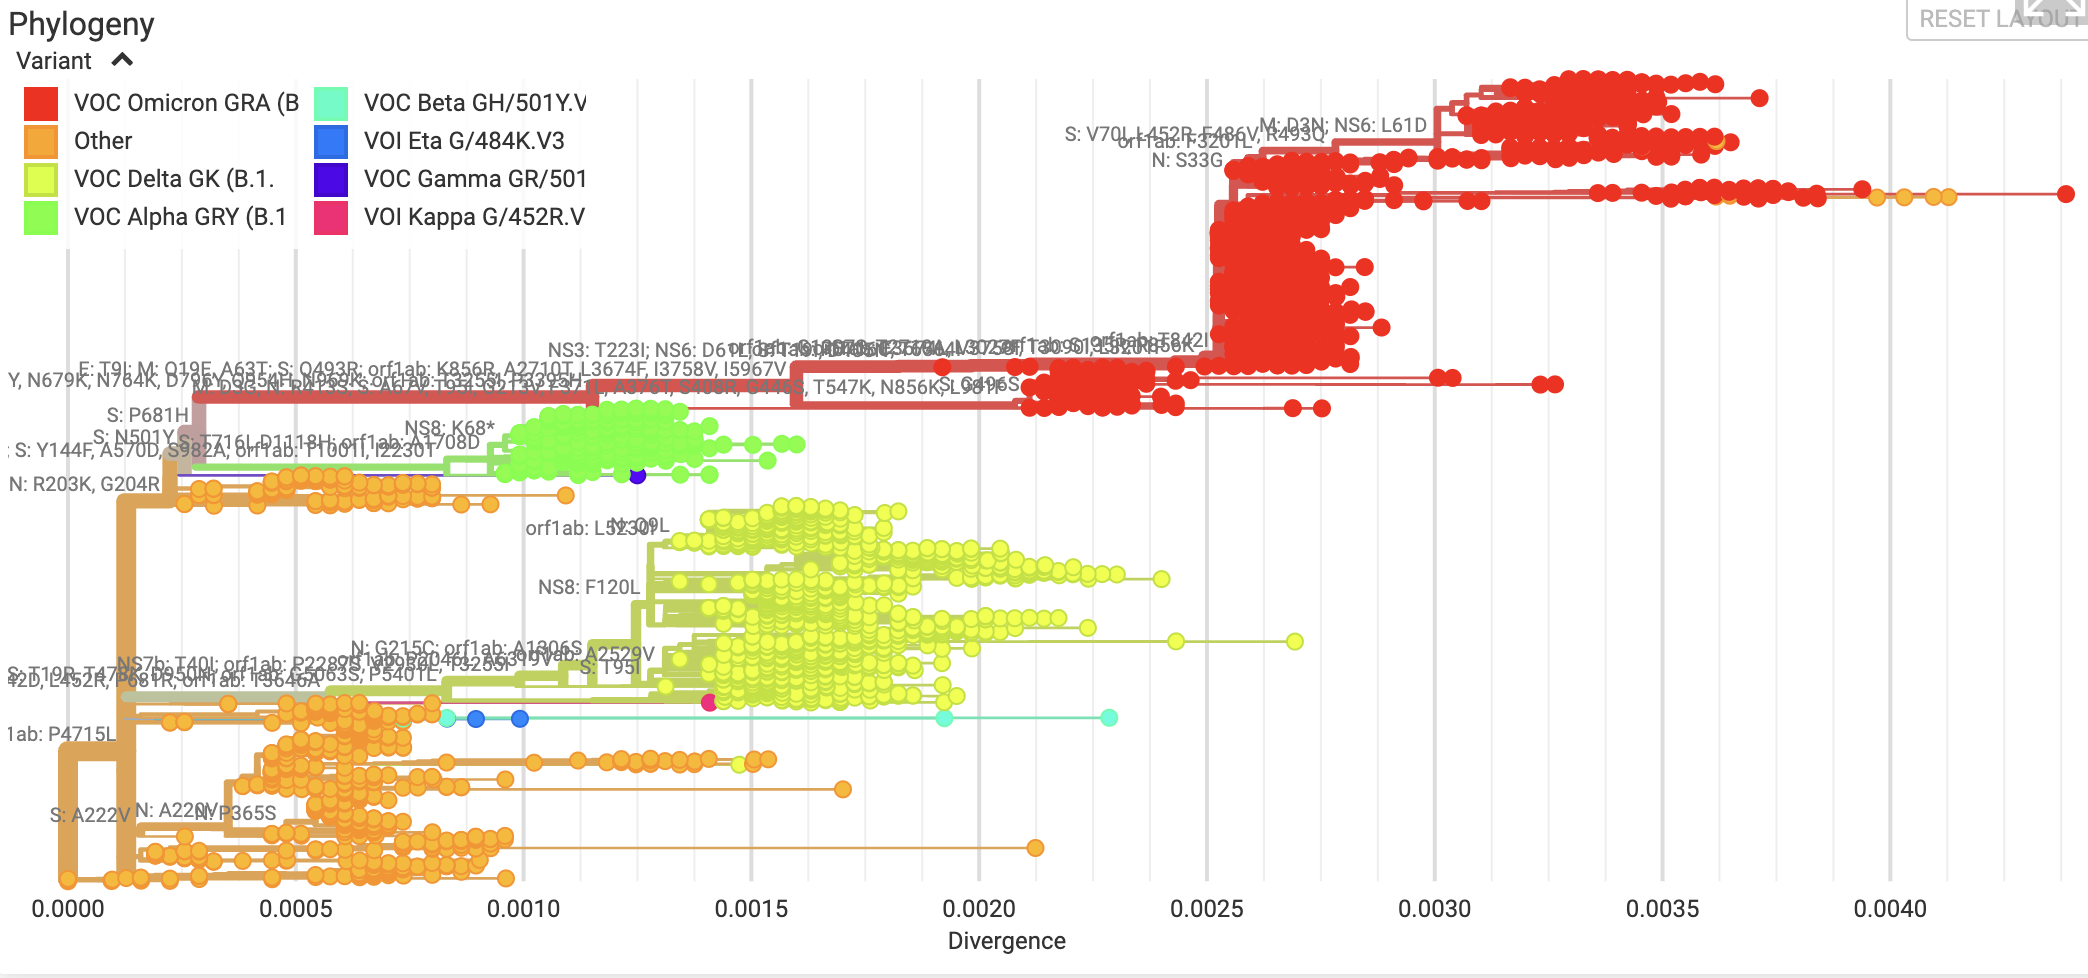
\includegraphics[width=0.7\textwidth,height=\textheight]{./Figures/DenmarkRectangularDivergence.png}
\caption{Divergence}
\end{figure}

What insights can you draw from each of the Denmark graphs?

What insights can you gain from comparing the two graphs?

What insights can you add from your country's or countries' graphs?

\hfill\break

Now change the tree to linear instead of rectangular and color code by variant. Use divergence.

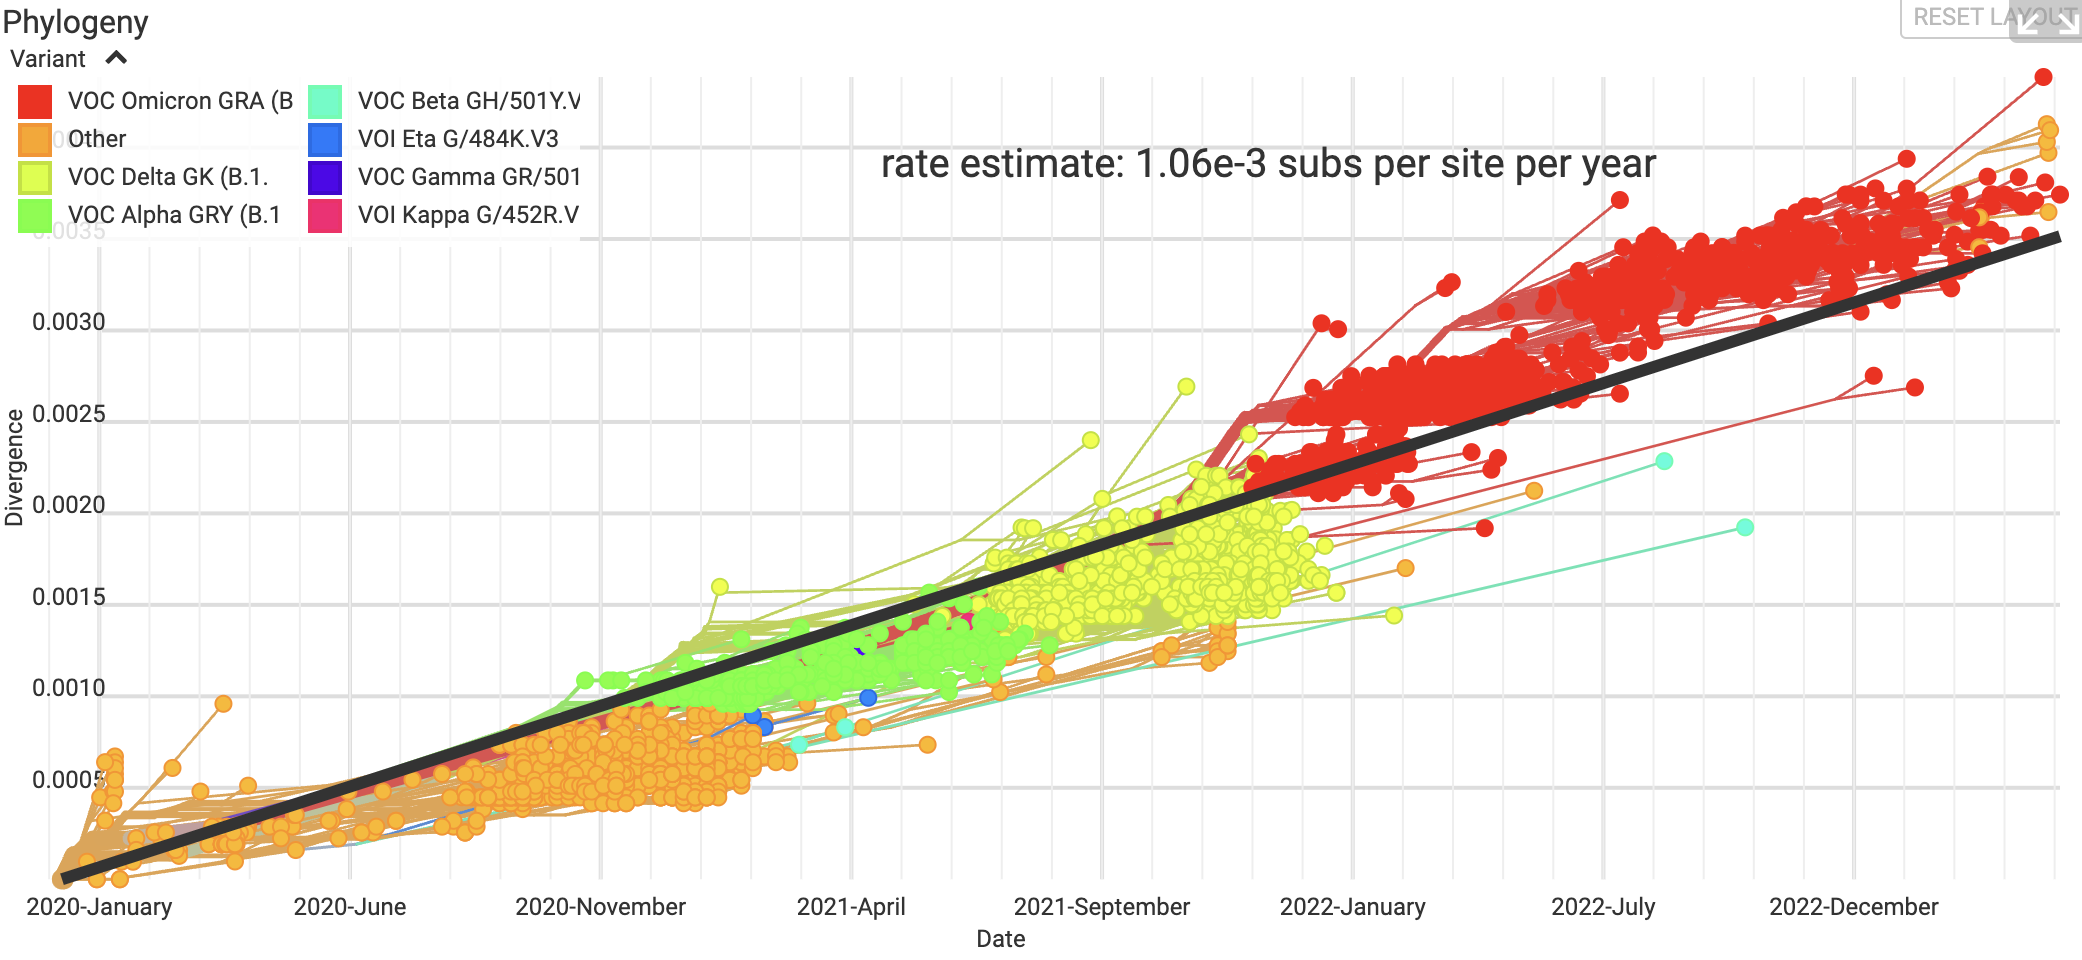
\includegraphics[width=0.7\textwidth,height=\textheight]{./Figures/DenmarkLinear.png}

What can you tell about the difference in divergence rates of omicron vs the other variants from the Denmark graph?

Do your country's/countries' graphs tell the same story?

Click for Possible Answer

\begin{verbatim}
  Omicron seems to diverge more rapidly as it is mainly above the average line while the other variants are mostly below it.
\end{verbatim}

\hfill\break

Now, explore other parameters with your country/countries.

What did you find that was interesting that you could share with the group?

Now, let's look at radial trees plotted by time and color-coded by variant and also by PANGO lineage.

\begin{figure}
\centering
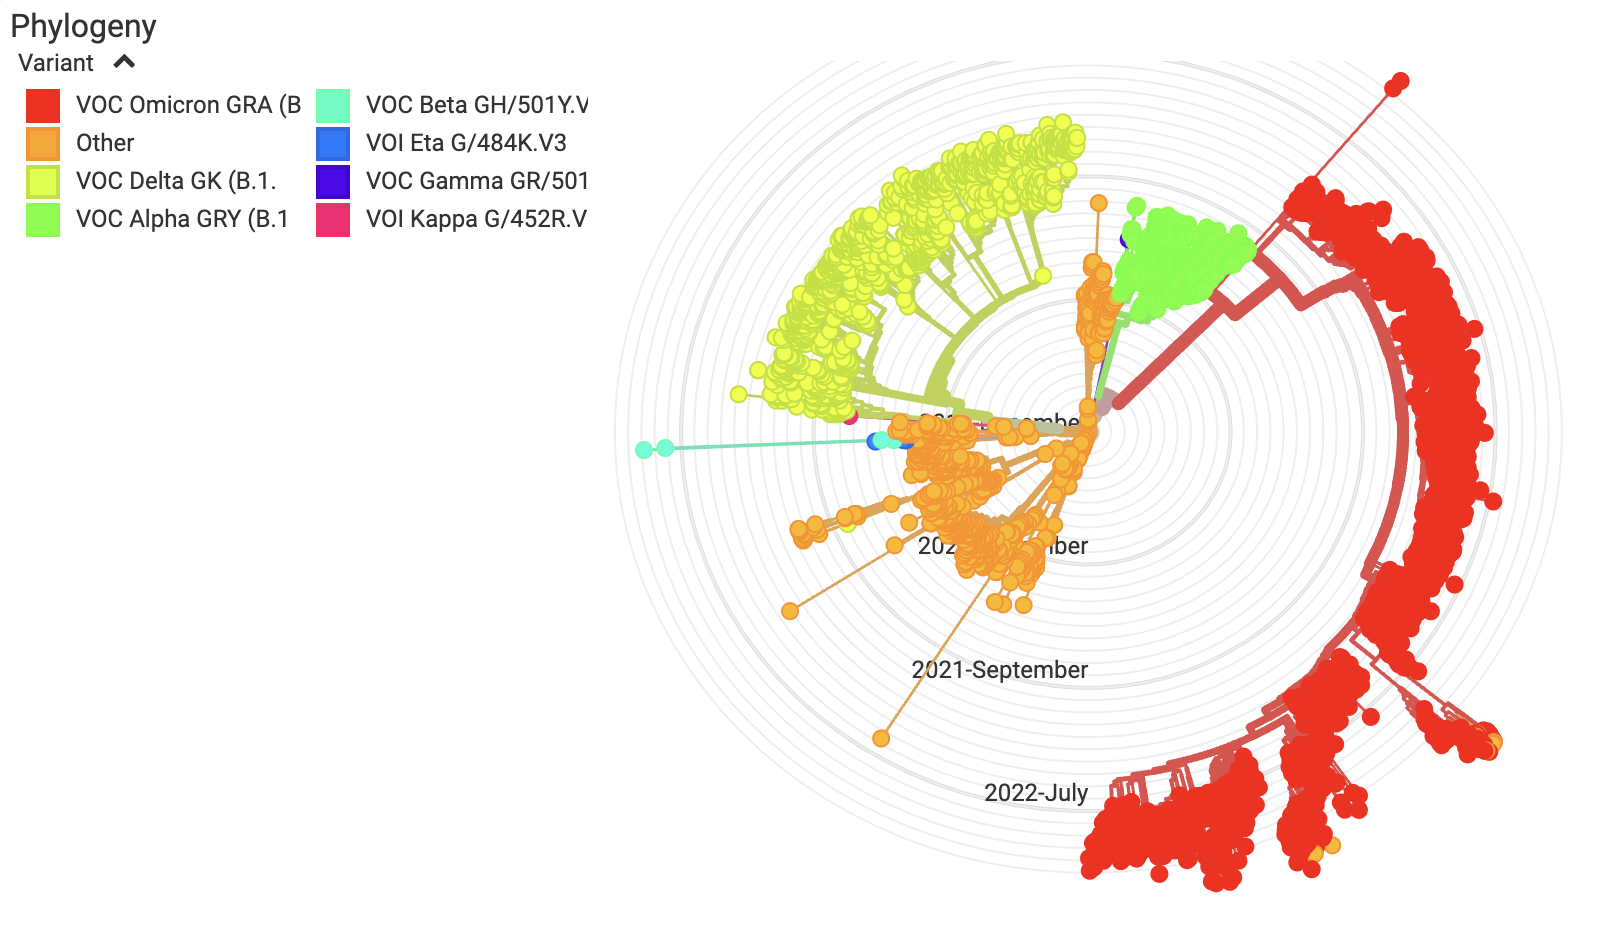
\includegraphics[width=0.7\textwidth,height=\textheight]{./Figures/DenmarkRadialTime.png}
\caption{Variant}
\end{figure}

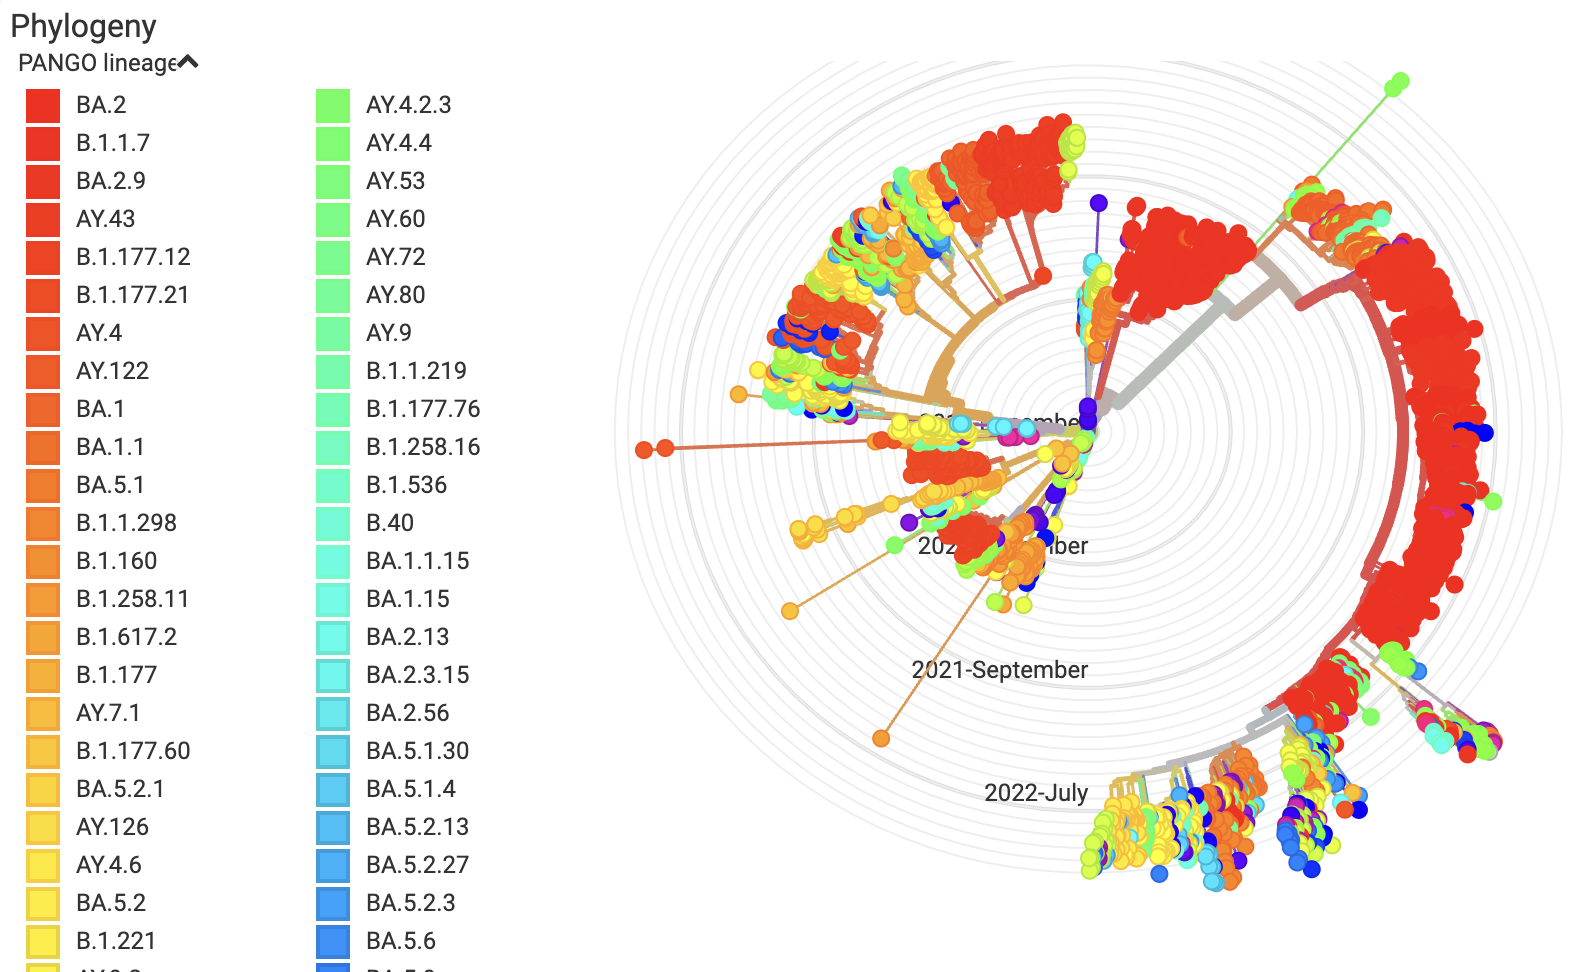
\includegraphics[width=0.7\textwidth,height=\textheight]{./Figures/DenmarkRadialTimePango.png}
What do you notice about the 2 trees? Is there anything interesting that you can share with the group in your countr/contries tree?

\hypertarget{genome-sequences}{%
\section{Genome sequences}\label{genome-sequences}}

Let's grab some sequences from our countries. I'll work through my countries but you can follow along with yours.

A few of my countries had hardly any genome sequences from NCBI.

\begin{quote}
Country. Sequences\\
Denmark 14\\
Norway 5\\
Sweden 616\\
\end{quote}

Click on ``Search''.


\includegraphics[width=0.5\textwidth,height=\textheight]{./Figures/search.png}

Check the complete box to limit your search to complete genomes. Type your country into the ``Location'' field and choose the appropriate text that pops up. Or choose the region of your country and click through to your country (ie. Europe, then Denmark).

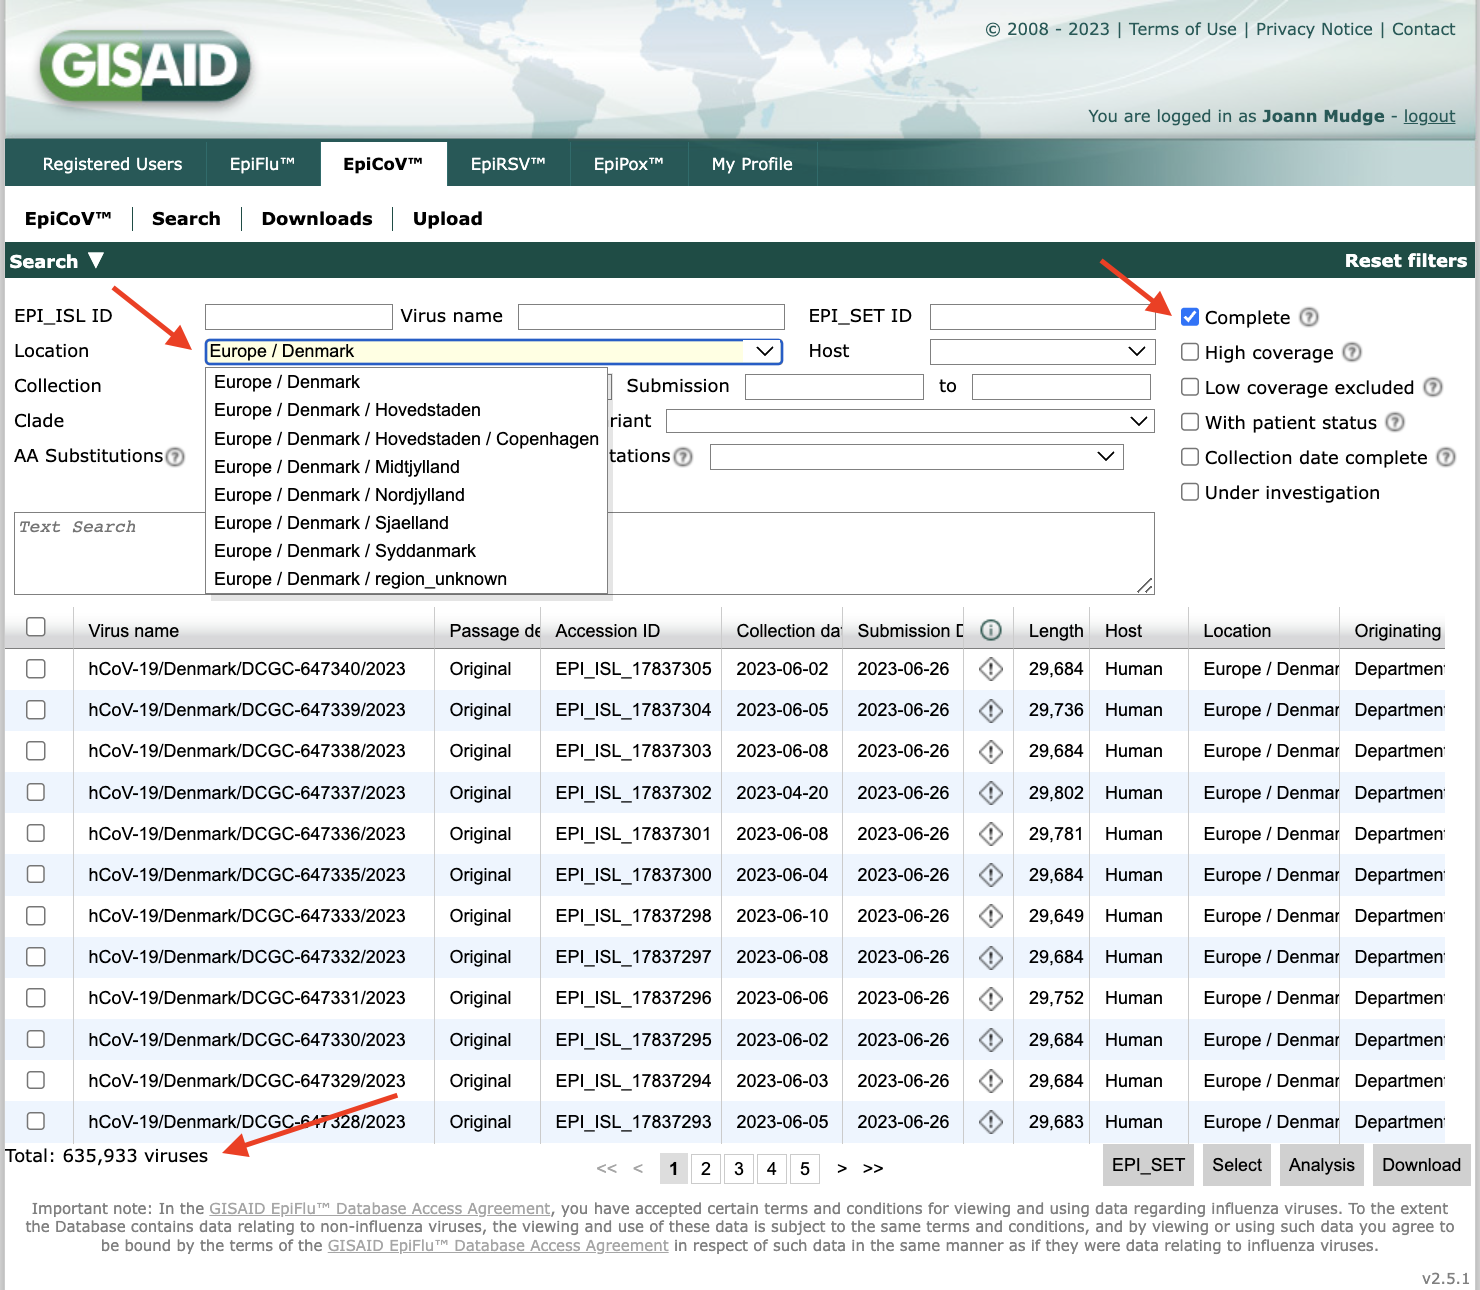
\includegraphics[width=0.7\textwidth,height=\textheight]{./Figures/DenmarkSearch.png}

How many did complete genome sequences did you find (see bottom left)?

Repeat for your 3 countries. Make sure you record this in your slides, including the date. This is a huge increase for Denmark from 14 in NCBI to 635,933 in GISAID!

\begin{quote}
Complete genome sequences (GISAID)
Denmark 635,933
Accessed 6/28/23
\end{quote}

GISAID limits us to downloading sequences 10,000 at a time. Let's zoom in on a smaller dataset.

In the same search, in the ``Variant'' field, choose XBB.1.16. This is the Arcturus subvariant.

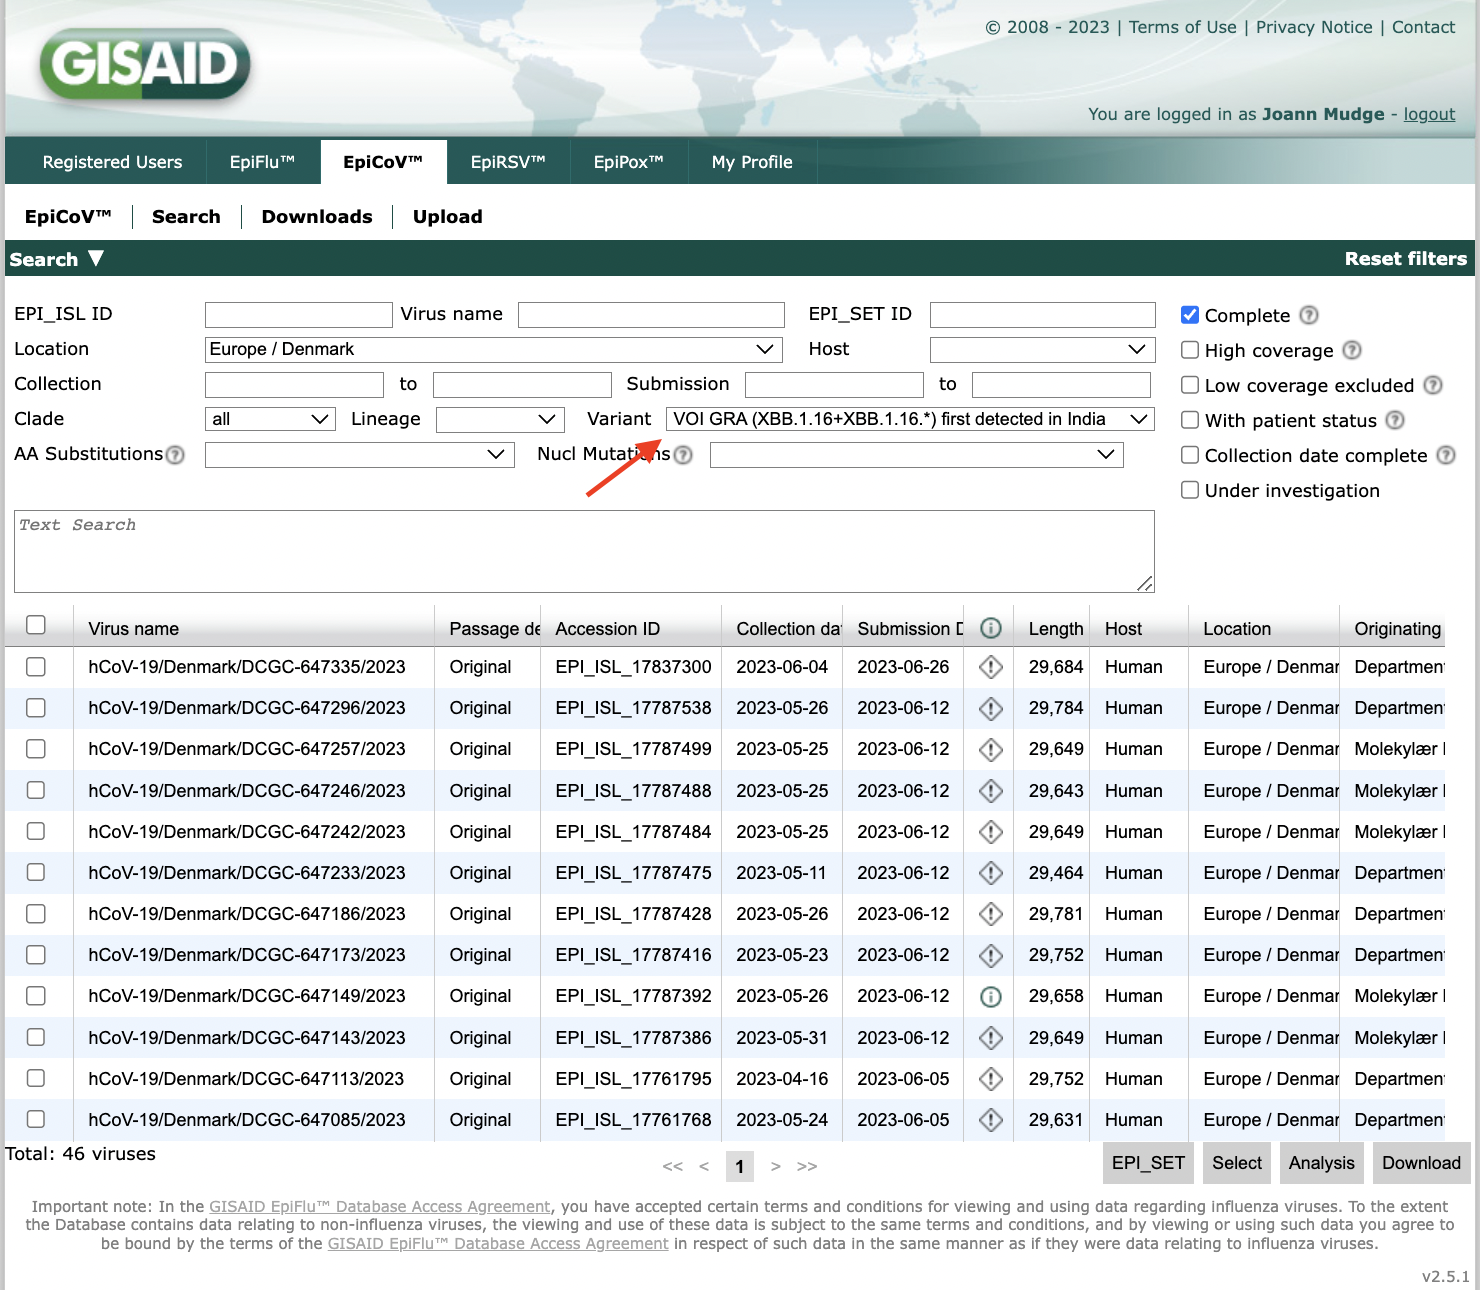
\includegraphics[width=0.7\textwidth,height=\textheight]{./Figures/gisaidSearch.png}
I got 46 for Denmark. Before we download these, we need to generate an EPI\_SET. GISAID requires you to cite all the people who contributed to any of the sequences that you are using in an analysis. So, any oral or poster presentation, or any manscript needs to acknowledge everyone who contributed genome sequences. This used to be a huge pain to gather all the information into a gigantic list. Now, they have made it easy EPI\_SETs, which gather the info for you and publish it to a DOI (a permanent Digital Object Identifier) that you can put on your publication to fulfill the acknowledgement requirements.

Select all sequences by clicking the checkbox near ``Virus Name''. Then, simply click on the ``EPI\_SET'' button on the bottom right. Then click ``Generate''.

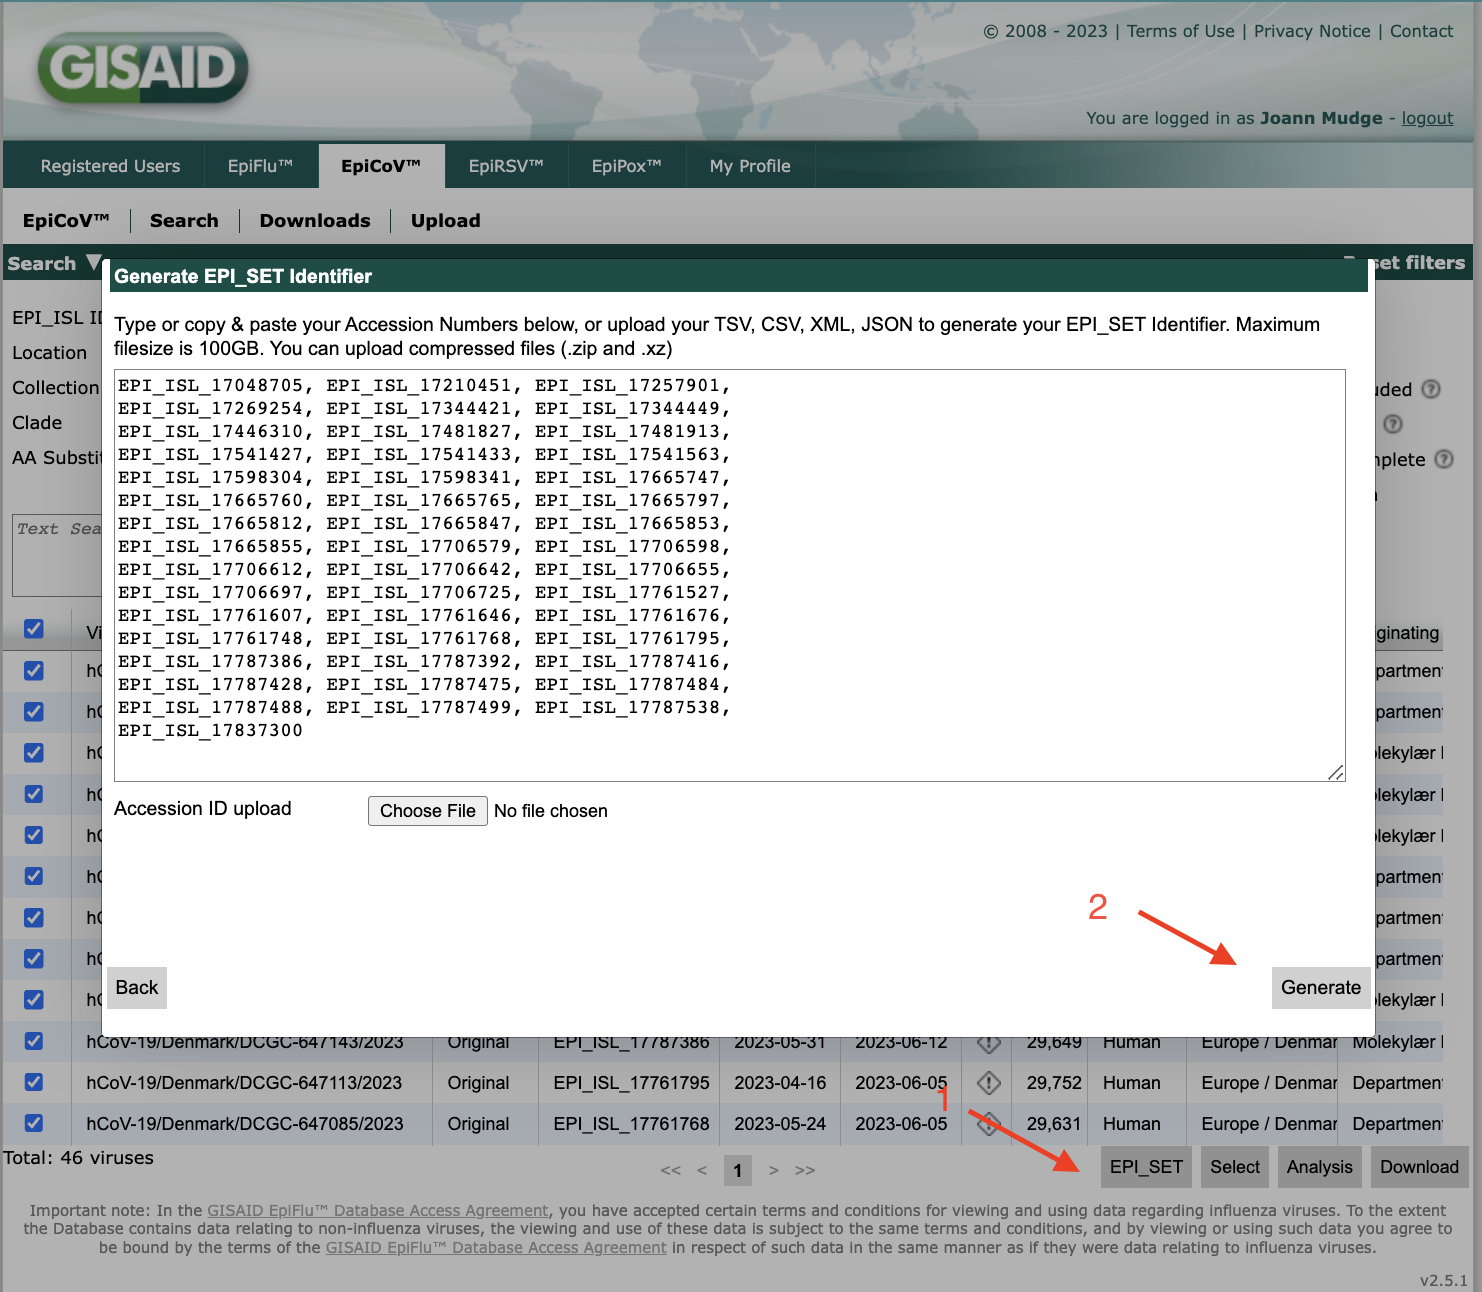
\includegraphics[width=0.7\textwidth,height=\textheight]{./Figures/episet.png}

It will email you the EPI\_set, with a link to the DOI and an attached supplemental table with text you can use in your publication.

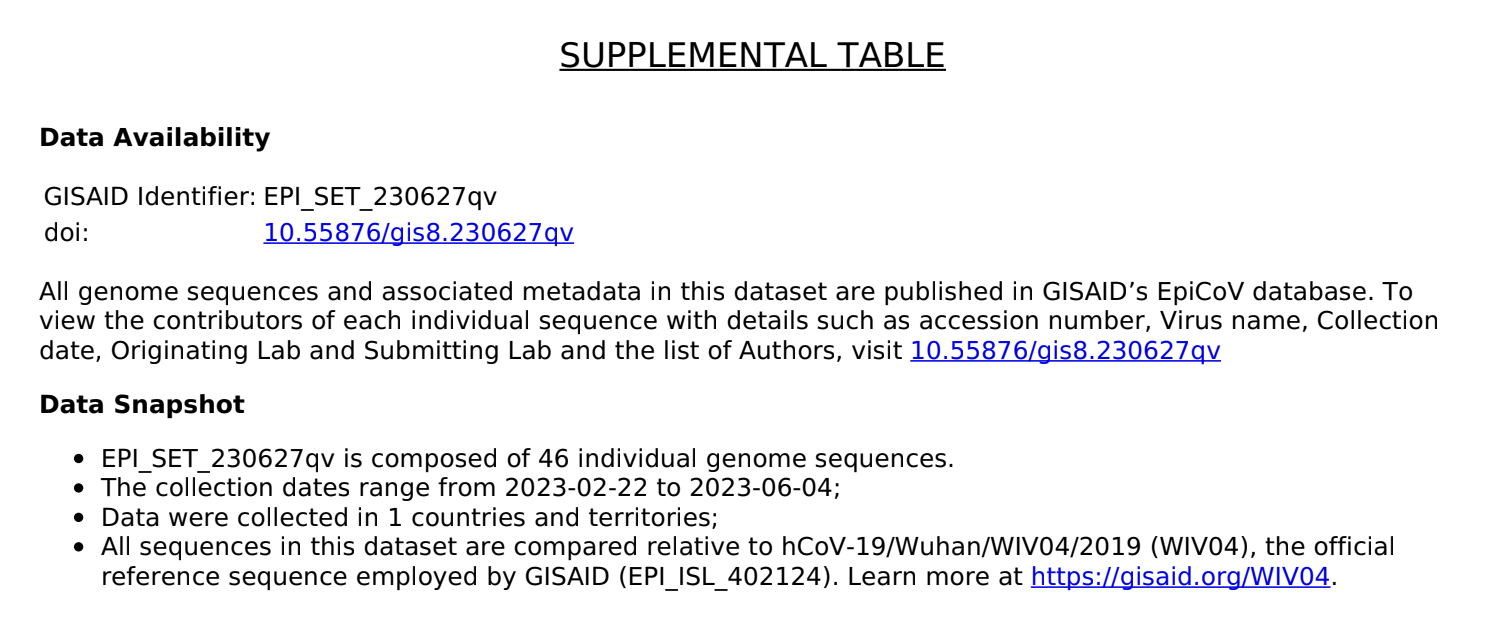
\includegraphics[width=0.7\textwidth,height=\textheight]{./Figures/SuppTable.png}

The DOI link will take you to a page that looks like the picture below. Hovering over each EPI number will pop up information about it (I'm hovering over the second to last number in the picture below).

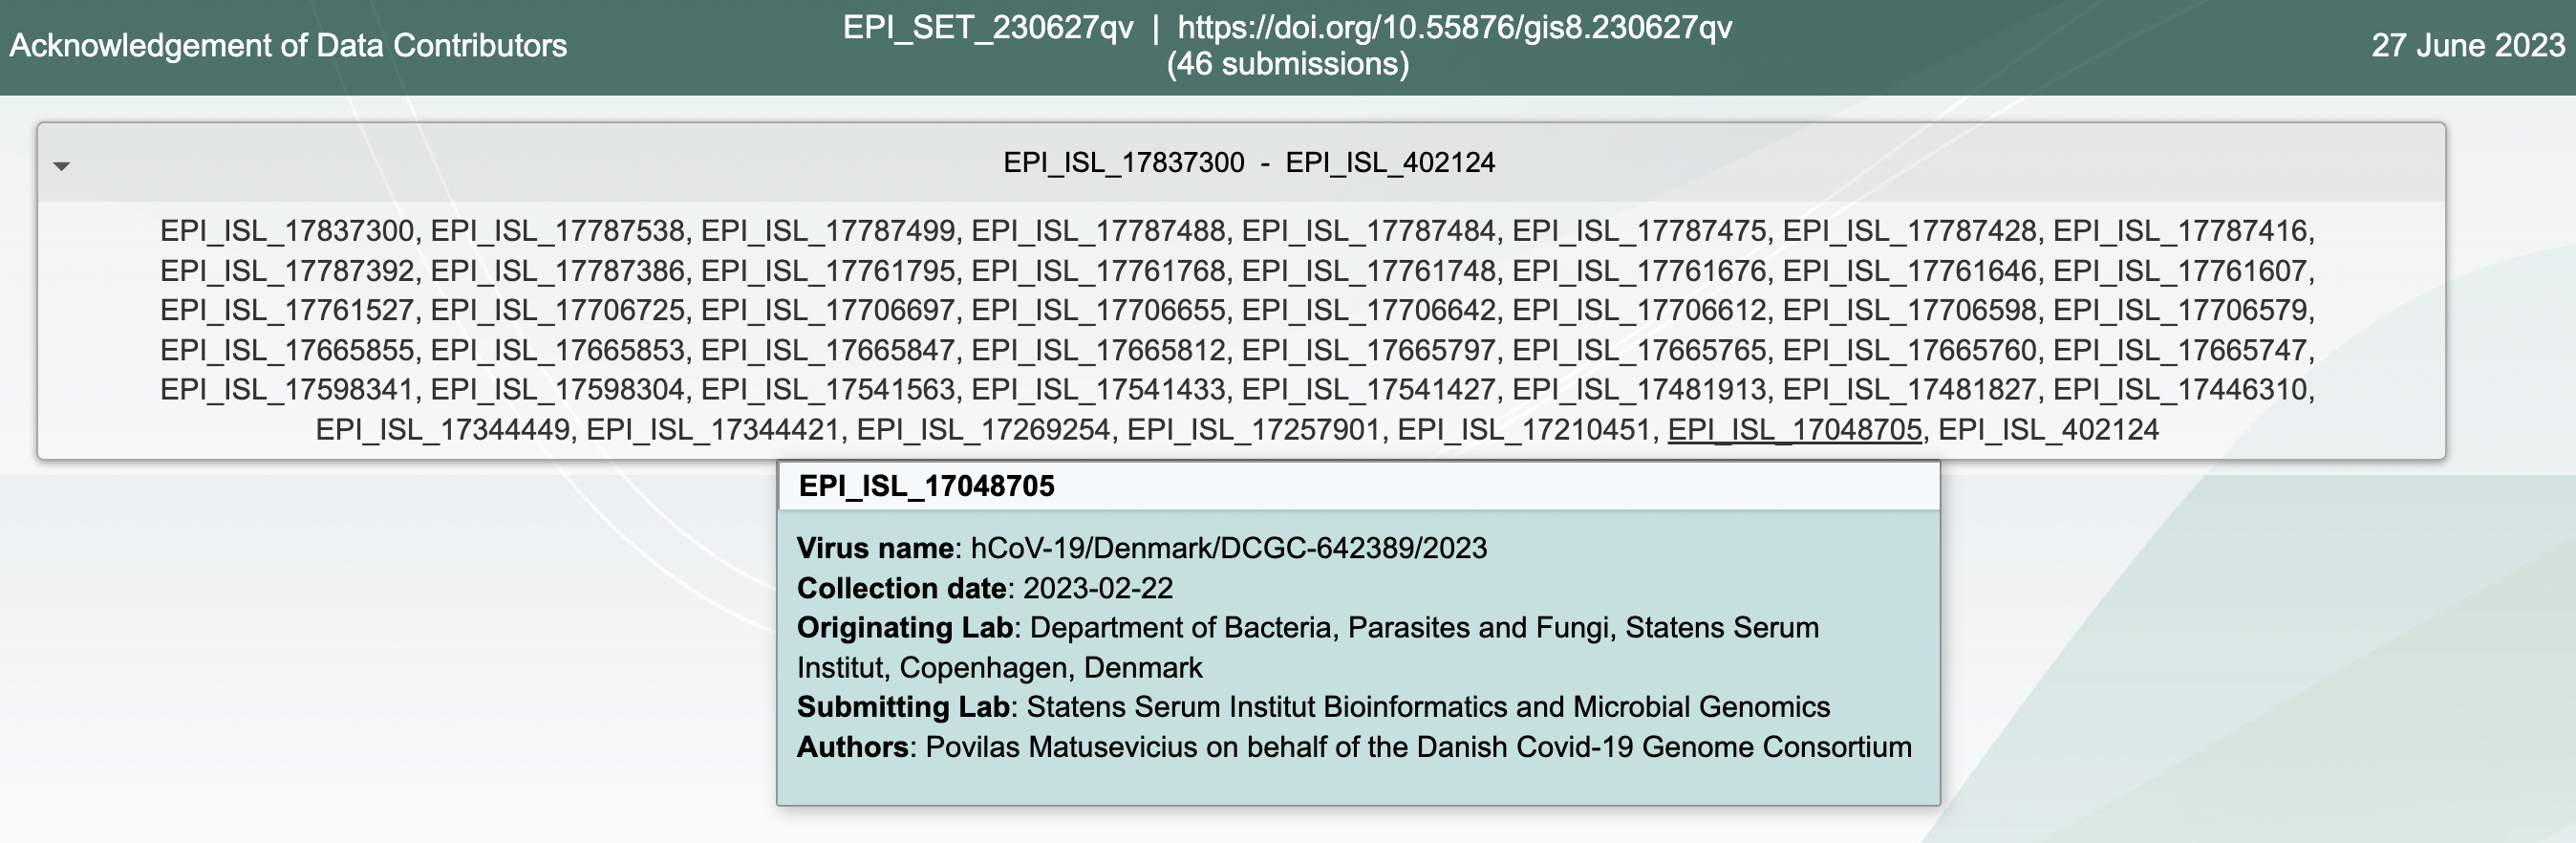
\includegraphics[width=0.7\textwidth,height=\textheight]{./Figures/AckDen.png}

Note that it also included the Wuhan reference.

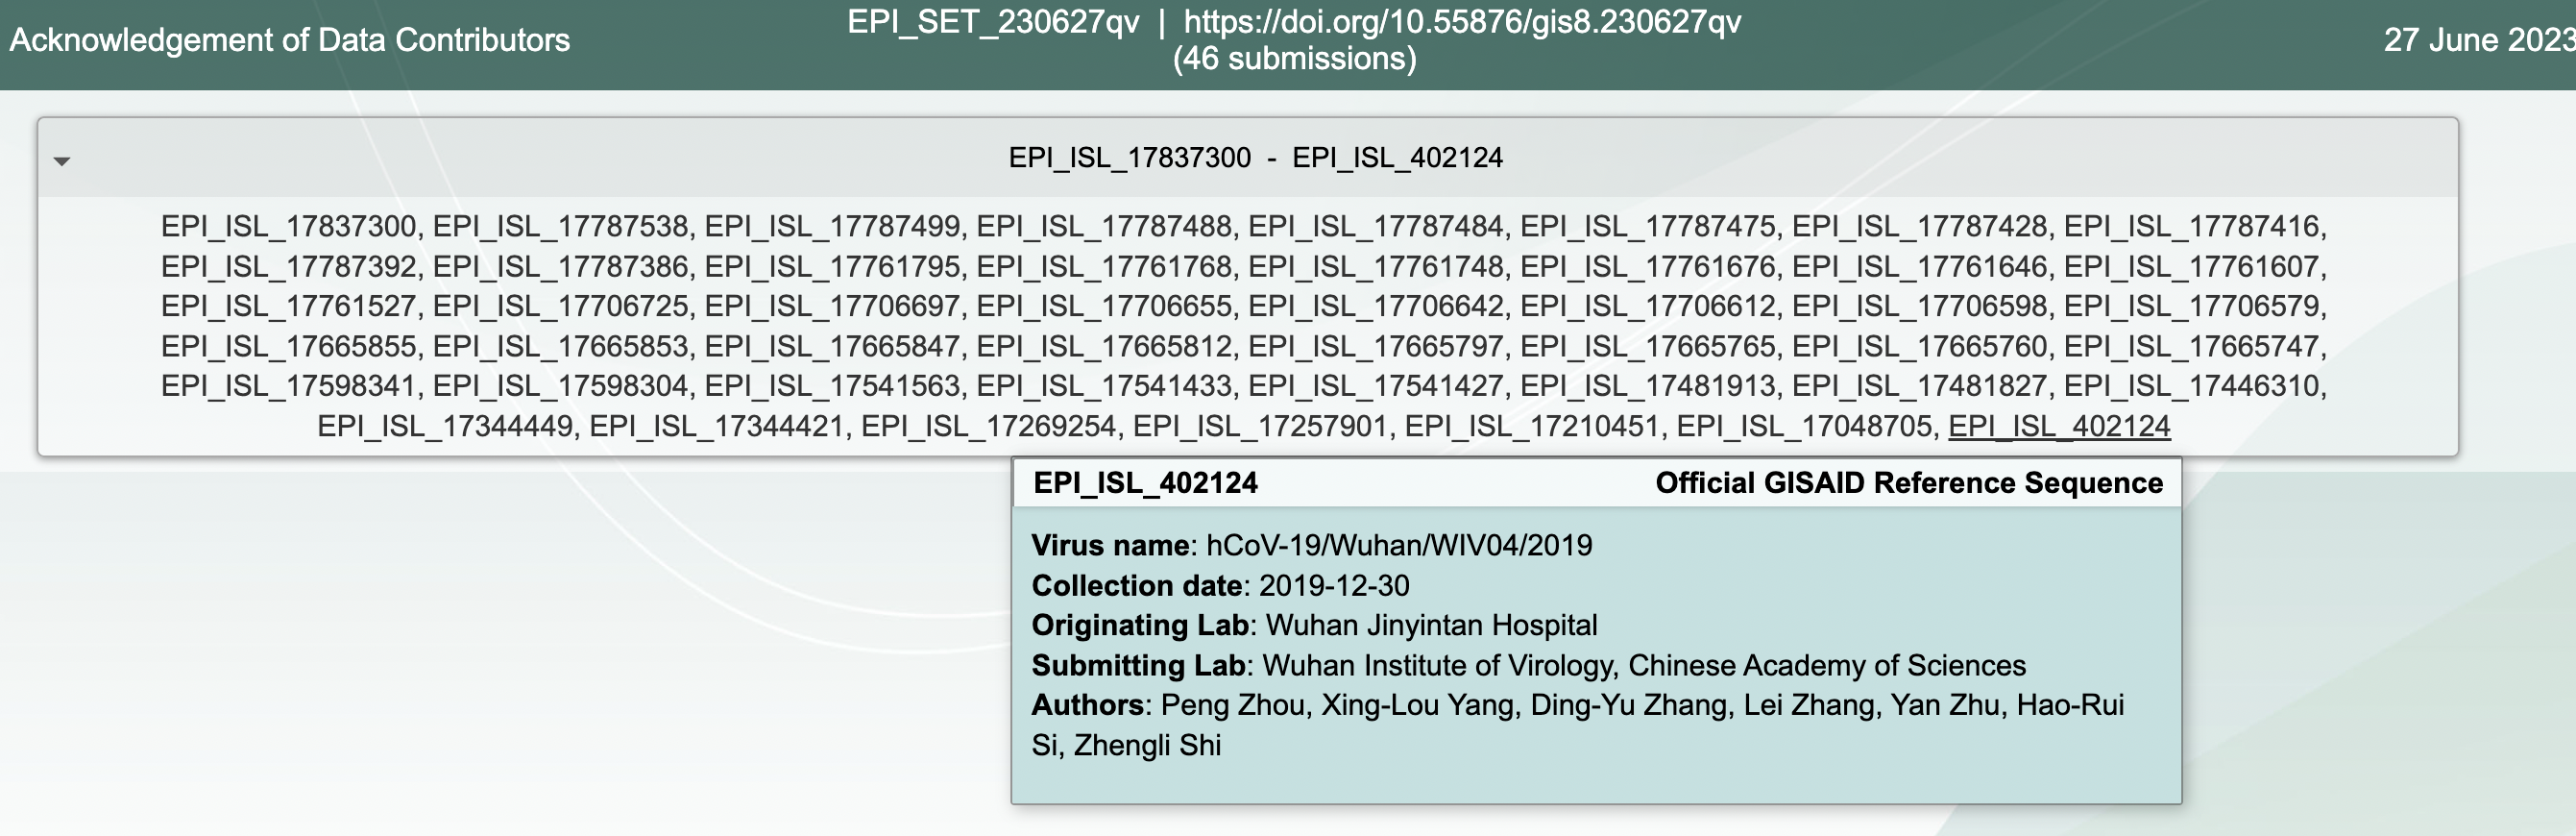
\includegraphics[width=0.7\textwidth,height=\textheight]{./Figures/AckWuhan.png}

Now click on ``Download'' to download the sequences.

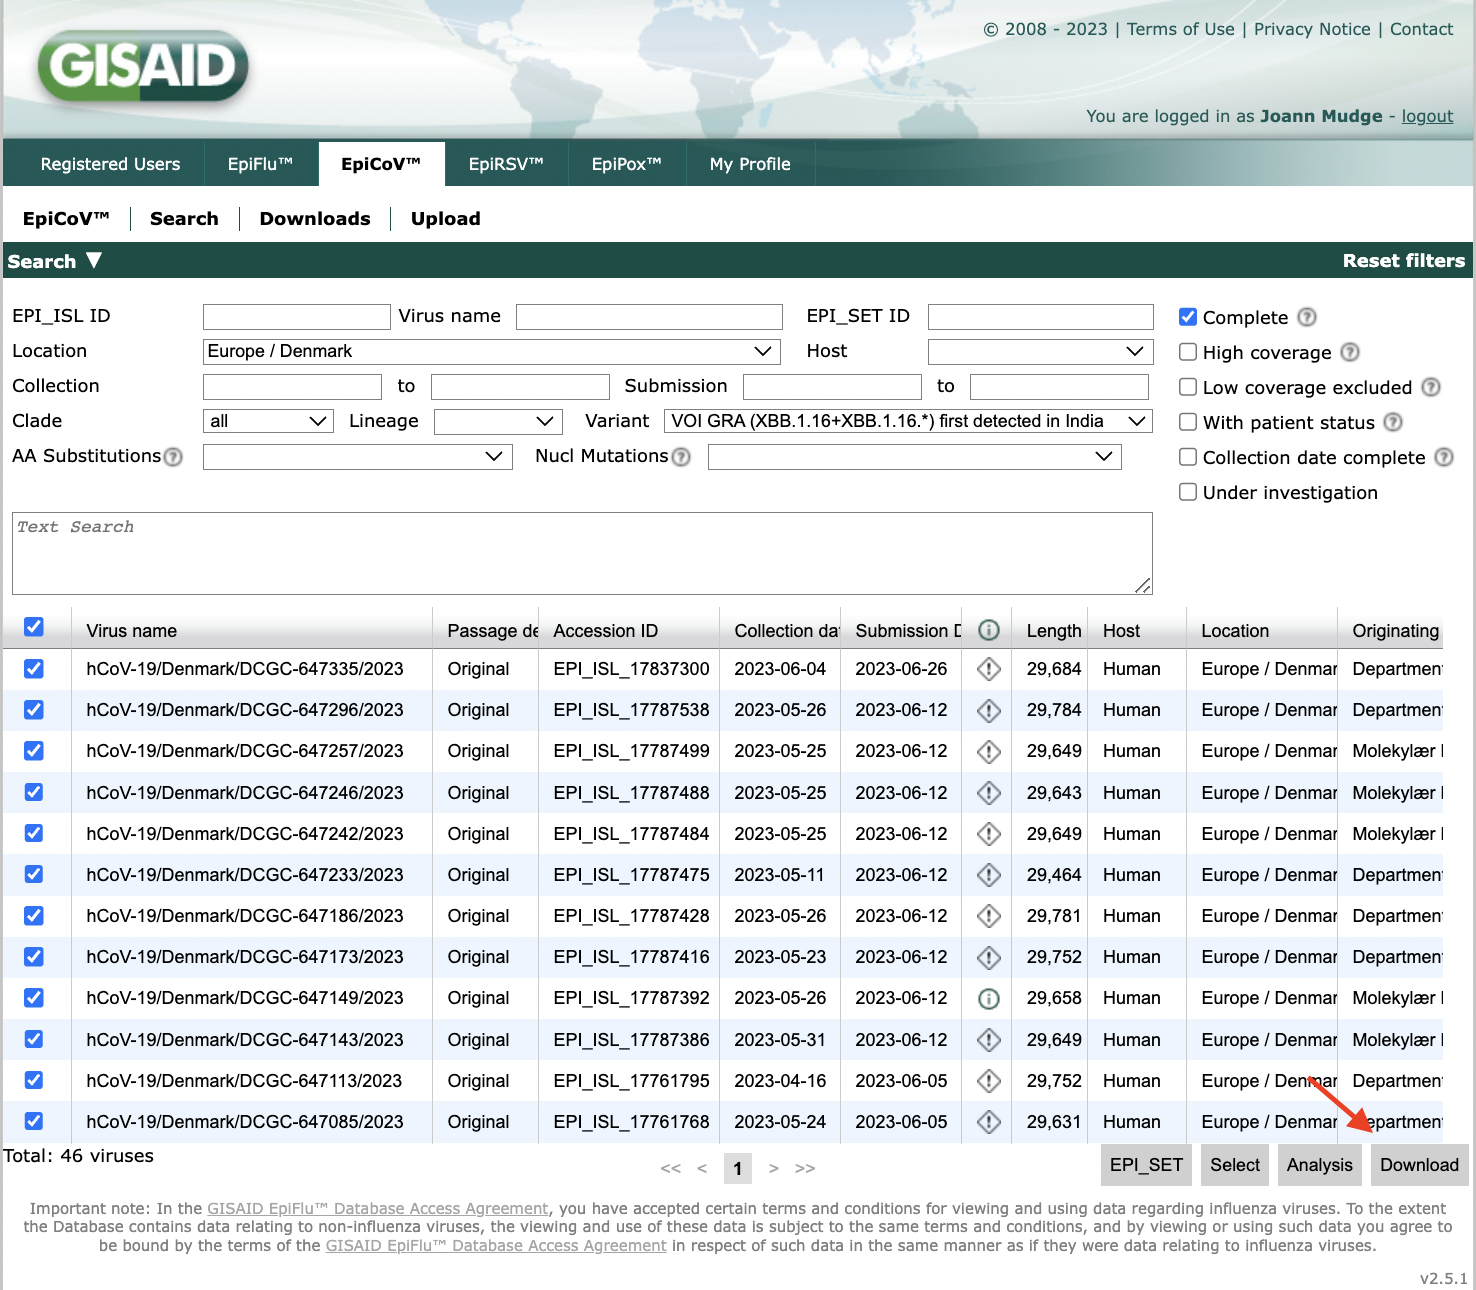
\includegraphics[width=0.7\textwidth,height=\textheight]{./Figures/download.png}

Change the name of the file to something that identifies the country the sequences came from and the fact that we limitted it to the Arcturus subvariant.

Repeat for your other 2 countries.

\hypertarget{upload-sequences}{%
\section{Upload sequences}\label{upload-sequences}}

Upload the sequences to the server.

\begin{enumerate}
\def\labelenumi{\arabic{enumi}.}
\tightlist
\item
  Copy your sequence files to the server.
\item
  Log onto the server (if you aren't alread logged on).
\item
  Create a new screen or reenter a previous screen.
\item
  Create a directory in your home directory called ``gisaid\_genomes''.
\item
  Move your sequence files into the gisaid\_genomes directory.
\item
  Navigate into the gisaid\_genomes directory.
\item
  Combine the Arcturus sequences from your 3 countries into a single fasta file.
\end{enumerate}

Click for Answers

\begin{verbatim}
  Adjust the commands below to reflect the filenames for your 3 countries and replace "jm" with your username.
  
1. scp -P 44111 *arcturus*fasta "jm@gateway.training.ncgr.org:/home/jm/"
2. ssh -p 44111 jm@gateway.training.ncgr.org
3. screen -S gisaid_genomes
4. mkdir ~/gisaid_genomes
5. mv *arcturus*fasta gisaid_genomes
6. cd gisaid_genomes
7. cat *arcturus*fasta > dns.arcturus.fasta
  
\end{verbatim}

\hfill\break

You should now have 4 fasta files in your tree directory: an arcturus fasta file for each of your 3 countries and the merged fasta file that has all 3 countries. Do an ``ls'' to doublecheck.

Count the number of sequences in all of your fasta files.

Click for Answers

\begin{verbatim}
grep -c '>' *fasta

  denmark_arcturus_gisaid_hcov-19_2023_06_27.fasta:46
  dns.arcturus.fasta:475
  norway_arcturus_gisaid_hcov-19_2023_06_27.fasta:34
  sweden_arcturus_gisaid_hcov-19_2023_06_27.fasta:395
\end{verbatim}

\hfill\break

Note: The large number of sequences in Sweden (395) compared to Denmark (46) and Norway (34) may represent more arcturus in Sweden but it might also represent sequencing of a greater fraction of COVID-19 patients in Sweden (a possibility I haven't looked into).

Now go back to GISAID and download another dataset from your 3 countries that you think might be useful in the story that you are putting together. You might limit it to a particular region of one of your countries or a particular time in the pandemic or a particular variant or amino acid change.

\hypertarget{multiple-sequence-alignment}{%
\chapter{Multiple Sequence Alignment}\label{multiple-sequence-alignment}}

\hypertarget{sars-cov-2-variant-genomes}{%
\section{SARS-Cov-2 variant genomes}\label{sars-cov-2-variant-genomes}}

We are going to line up some SARS-CoV-2 genomes so that their corresponding nucleotides all match up and their genes start and stop in the same place. This will involve adding in gaps here and there where some sequences have insertions relative to other sequences. We'll start with a file that has genome sequences for some SARS-CoV-2 variants.

Do the following:
On the server, create a directory called sars-variants in your home directory.
Navigate into that directory
Soft link to the file /home/jm/sarsdata/sars-cov-2-variants.fasta

Click for Answers

\begin{verbatim}
  mkdir ~/sars-variants
  cd ~/sars-variants
  ln -s /home/jm/sarsdata/sars-cov-2-variants.fasta .
\end{verbatim}

\hfill\break

How many sequences are there in the file?
Which SARS-CoV-2 variants are there?

Click for Answers

\begin{verbatim}
  grep -c '>' sars-cov-2-variants.fasta
  grep '>' sars-cov-2-variants.fasta
  
  > Original variant (Wuhan-Hu-1)
  > Alpha
  > Delta
  > Omicron
\end{verbatim}

\hfill\break

We'll start with a java tool which will allow us to do an alignment and to visualize it.

Dowload the sars-cov-2-variants.fasta file onto your computer.

Install Jalview (\url{https://www.jalview.org/}). Click on download and choose the windows or mac version and install it.

Open up Jalview.

Close all the windows except the blank window at the back.

Go to main menu at the very top. Choose File \textgreater{} Input Alignment \textgreater{} From File -
Then choose the sars-cov-2-variants.fasta file.

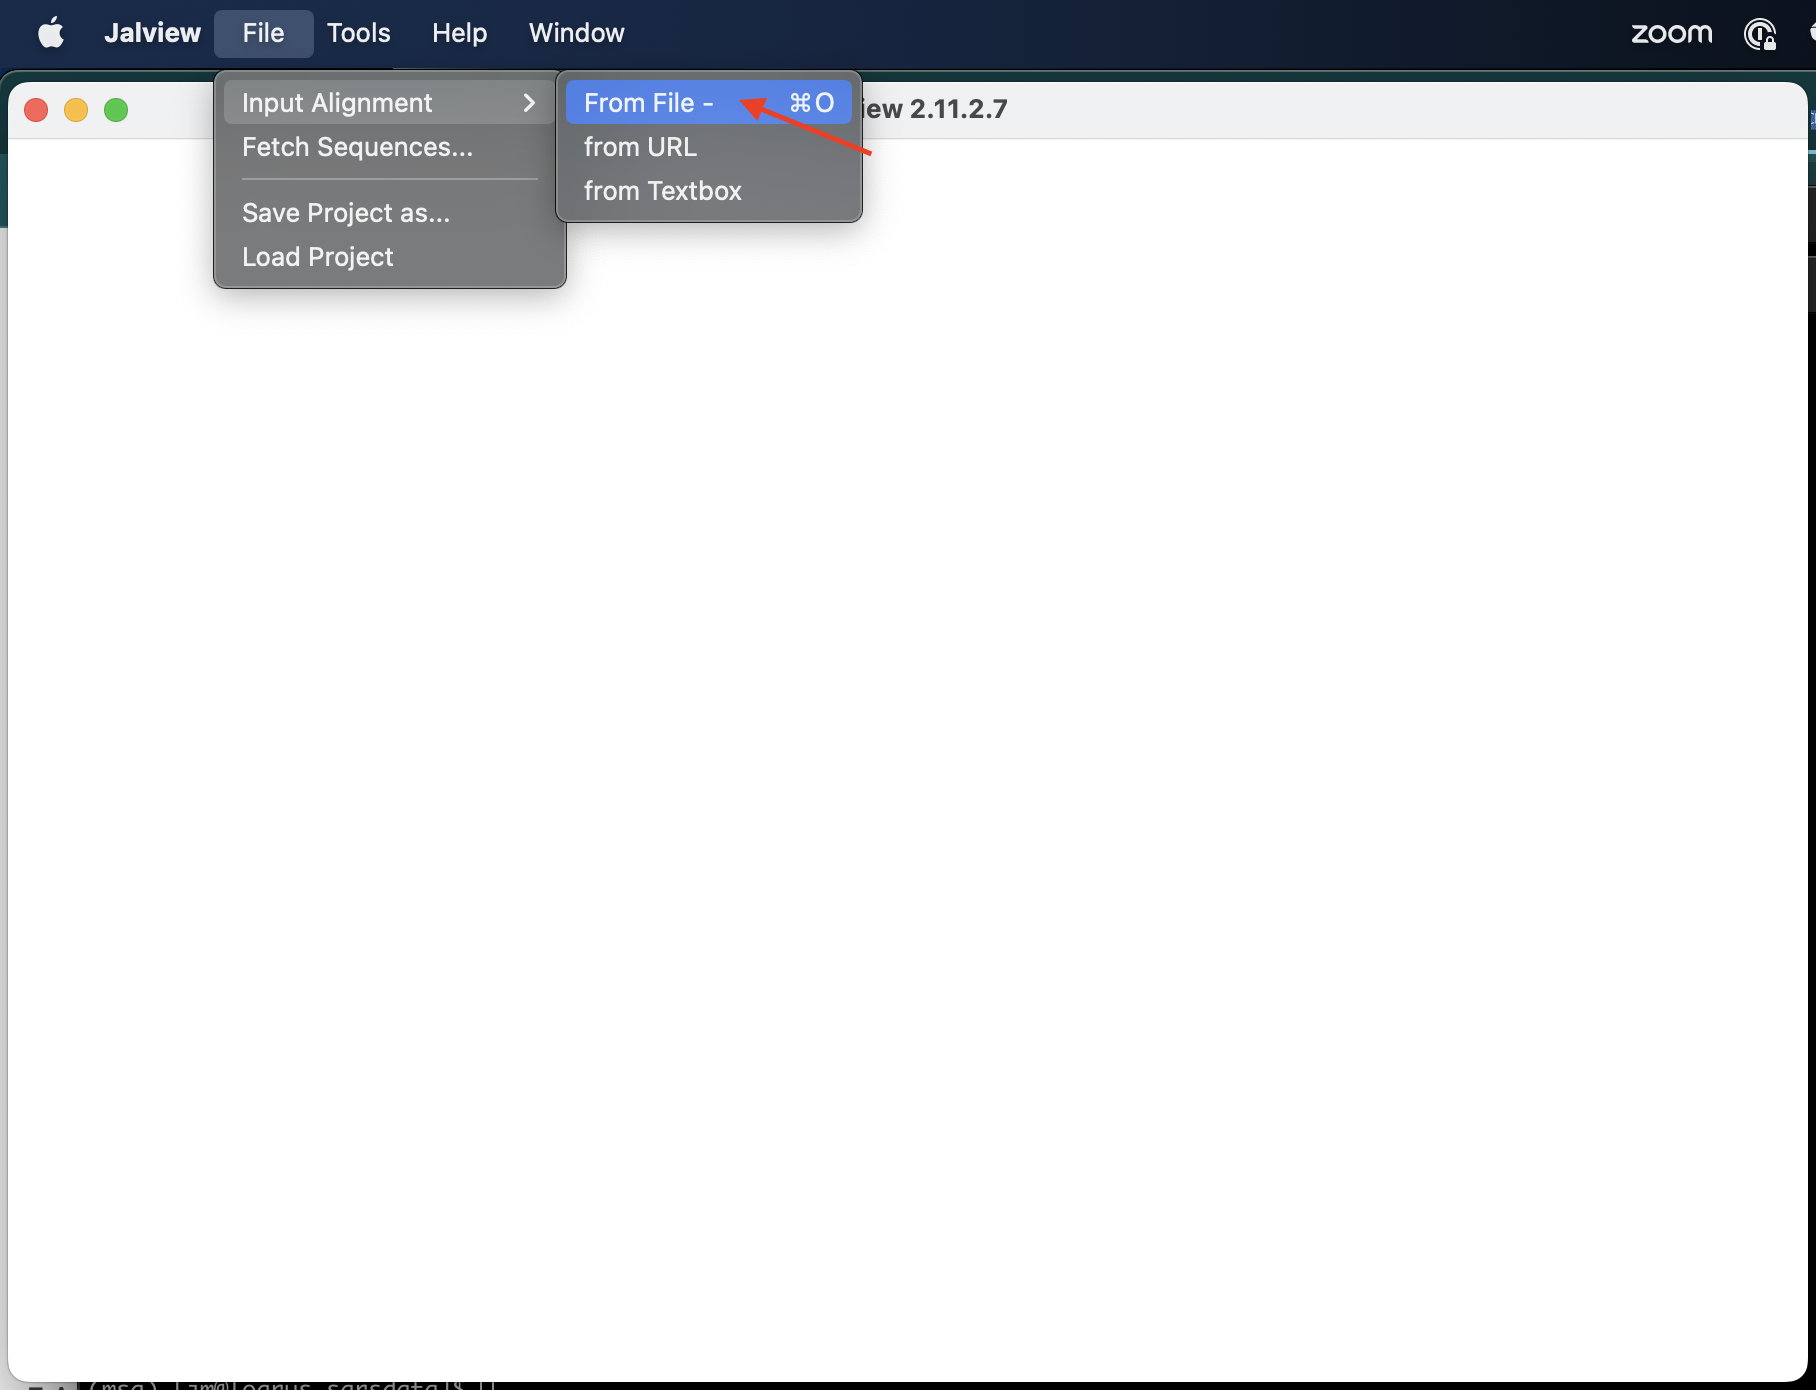
\includegraphics[width=0.7\textwidth,height=\textheight]{./Figures/open.png}
It is expecting an aligned fasta file and we are opening up a fasta file that hasn't been aligned yet. Let's take a look at it in its unaligned form, first.

Color the sequences by nucleotide by choosing:
Colour \textgreater{} Nucleotide

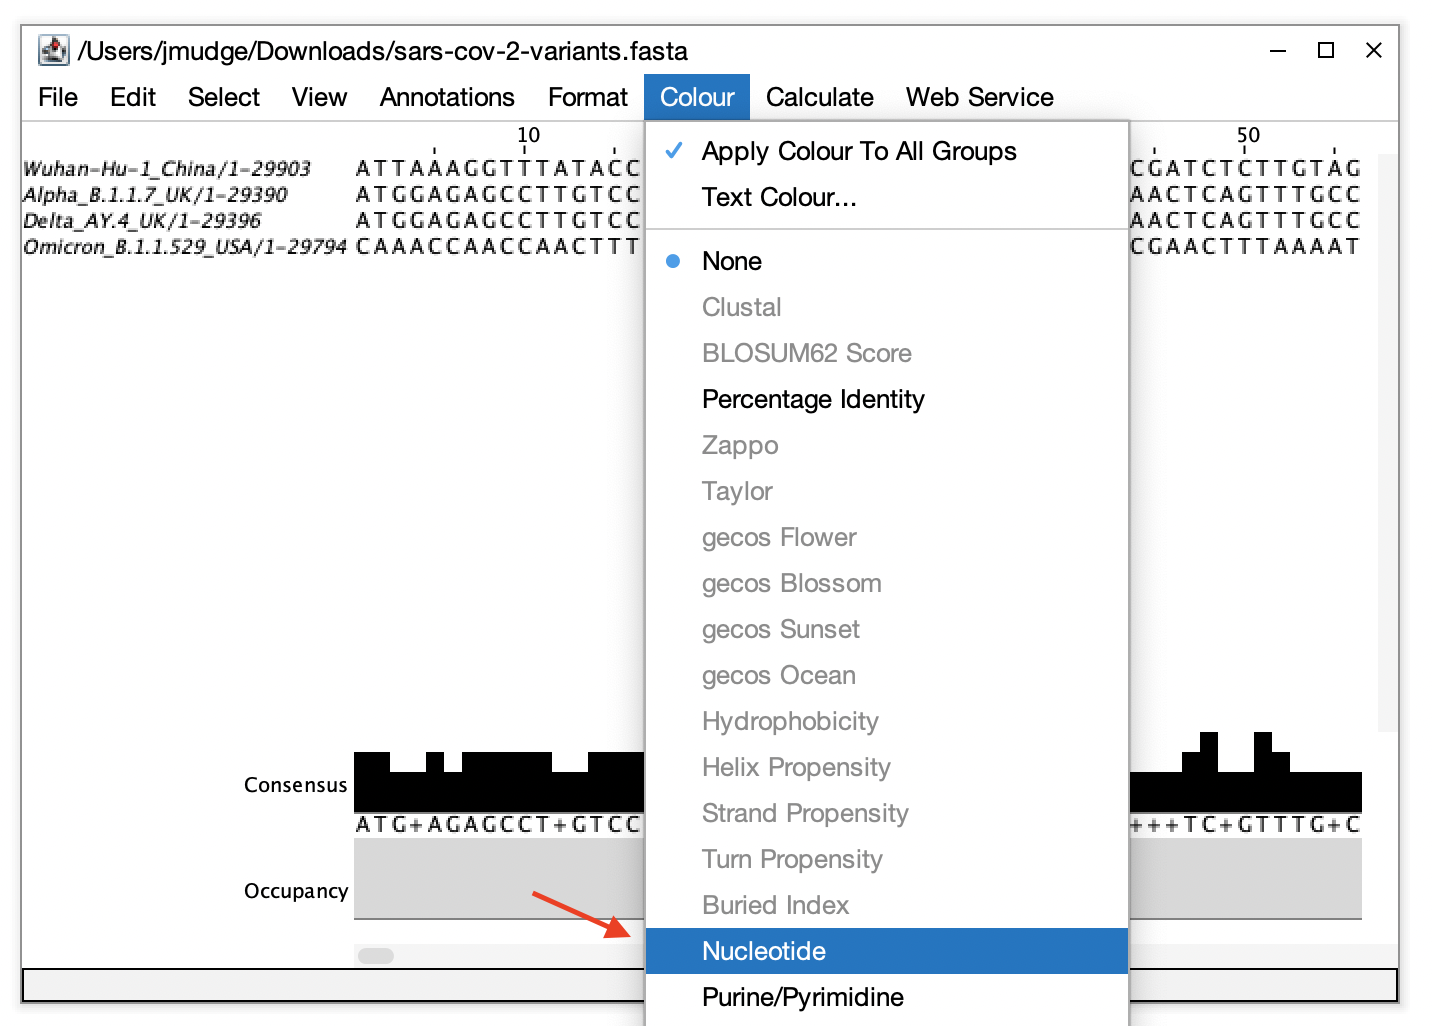
\includegraphics[width=0.7\textwidth,height=\textheight]{./Figures/color.png}

Alpha and Delta line up pretty well but the other two are way off because their sequence is shifted relative to Alpha and Delta.

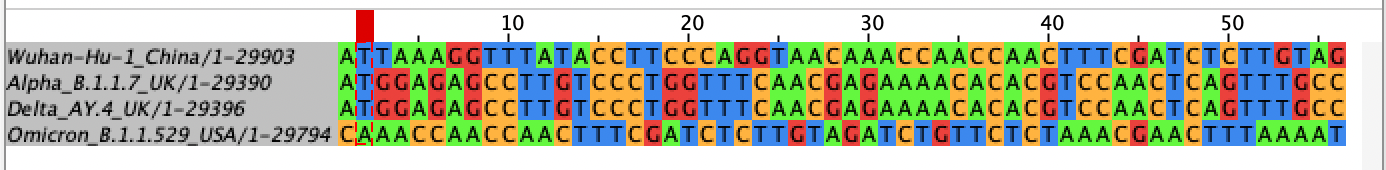
\includegraphics[width=0.7\textwidth,height=\textheight]{./Figures/unaligned.png}

So, let's align them now. We'll use the MAFFT (Multiple Alignment using Fast Fourier Transform) aligner, which is a very fast multiple sequence aligner.

Choose:
Web Service \textgreater{} Alignment \textgreater{} Mafft with defaults

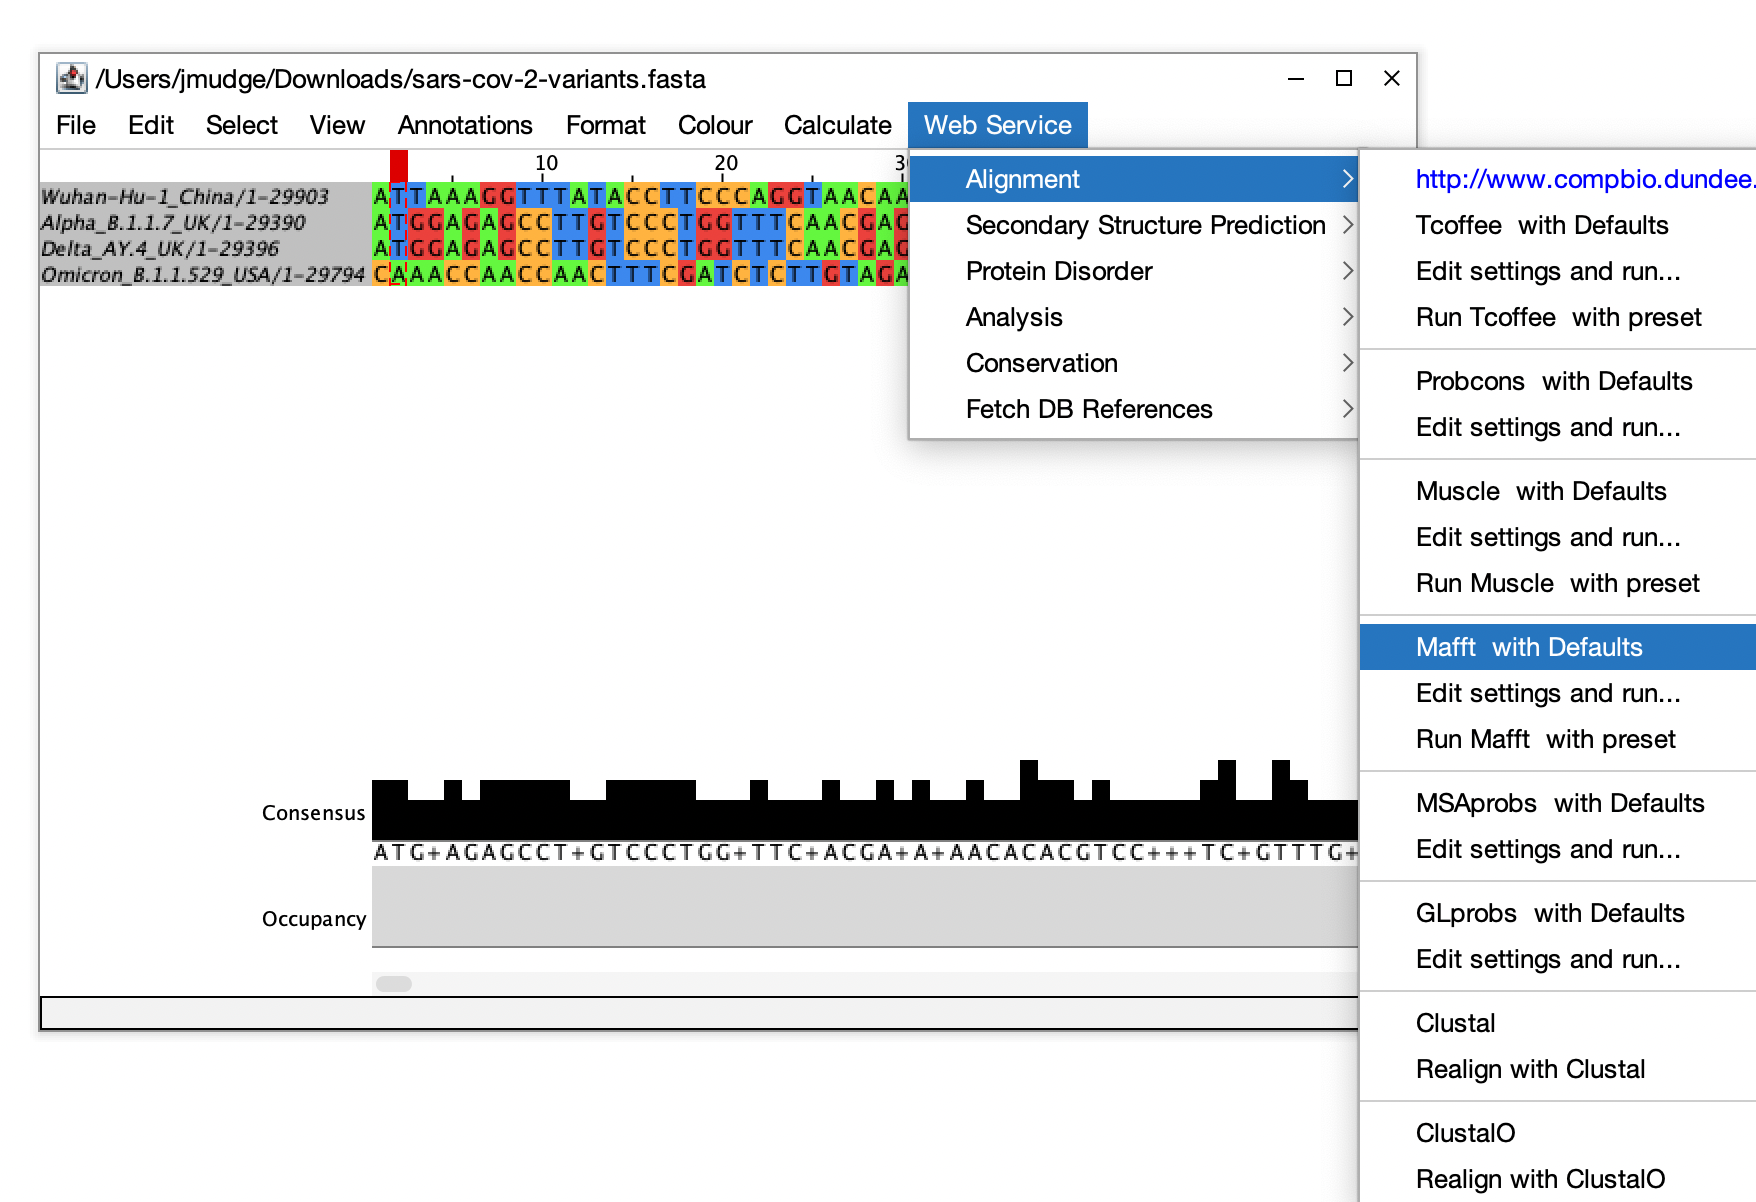
\includegraphics[width=0.7\textwidth,height=\textheight]{./Figures/mafft_jalview.png}

Go ahead and color by nucleotide again.

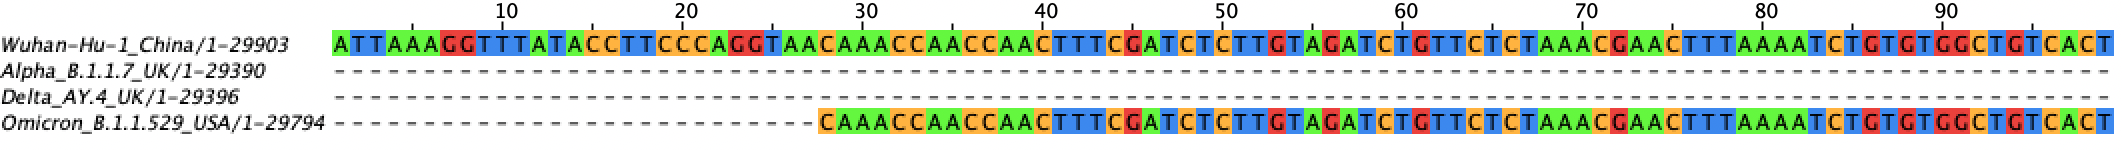
\includegraphics[width=0.7\textwidth,height=\textheight]{./Figures/aligned.png}

Now the original (Wuhan-Hu-1) and the Omicron are lining up. The dashes mean that there is no sequence there. In other words, not all the variant genomes were sequenced and assembled all the way to the ends of the RNA genome molecule. Scroll to the right until you can see sequence in all four variants.

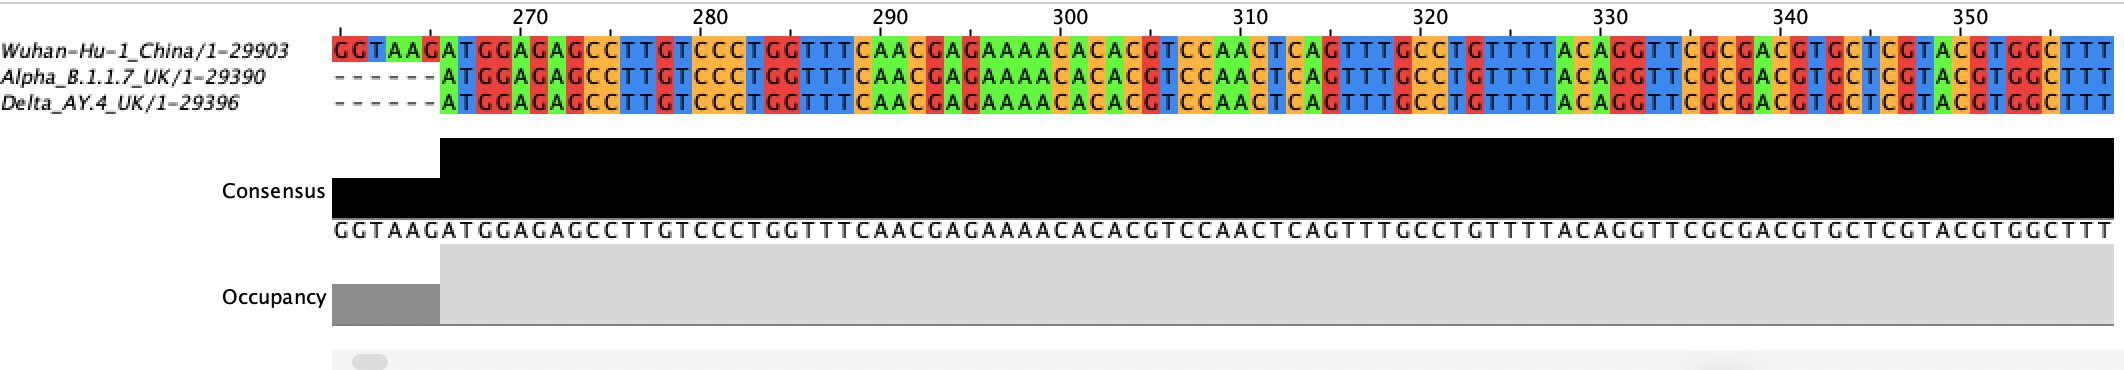
\includegraphics[width=0.7\textwidth,height=\textheight]{./Figures/consensus.png}

They all start to look identical here. The consensus and occupancy tracks can tell you quickly whether everything has sequence in that region (occupancy) and whether they all have the same nucleotide (consensus).

Scroll all the way to the right to see the end of the chromosome. Did every genome assembly make it to the end?

Click for Answers

No, they didn't.

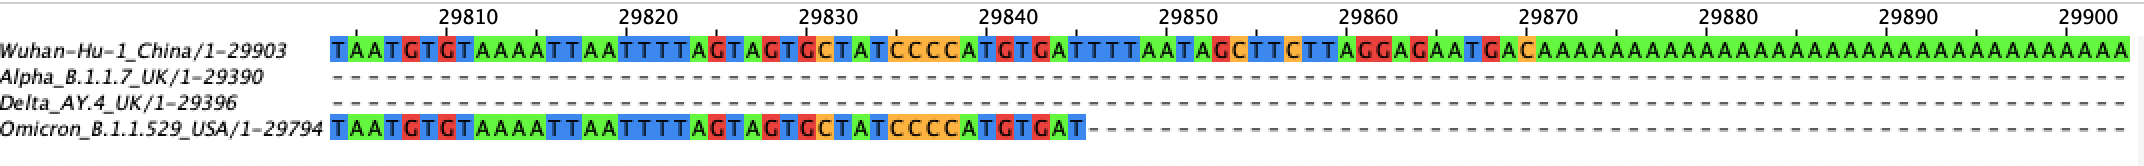
\includegraphics[width=0.7\textwidth,height=\textheight]{./Figures/chrend.png}

\hfill\break

Take a look at the overview window.
View \textgreater{} Overview

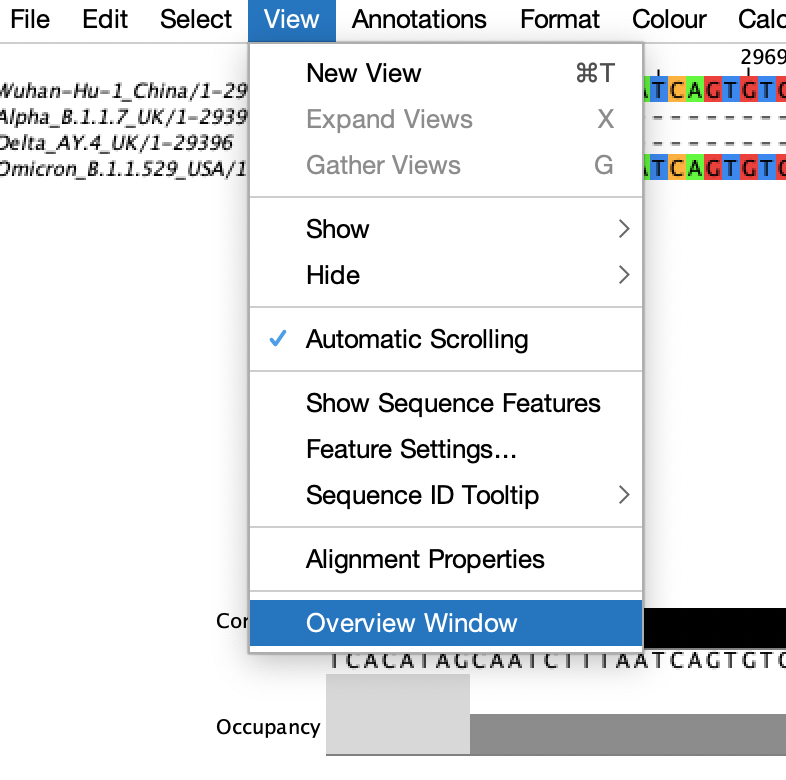
\includegraphics[width=0.4\textwidth,height=\textheight]{./Figures/overview.png}

Expand it by hovering over the bottom right-hand corner until the cursor changes, then click and drag to make it bigger.

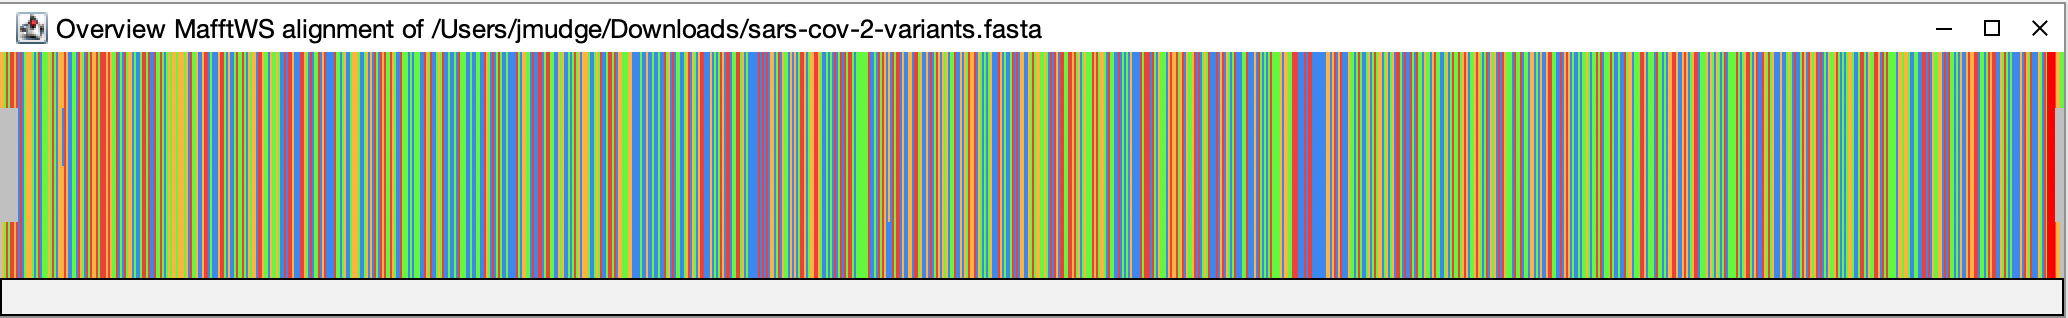
\includegraphics[width=0.7\textwidth,height=\textheight]{./Figures/overview_window.png}

This has all four genome one on top of each other across the whole genome sequence (\textasciitilde30kb).

If you click on the overview, it will take you to the corresponding position in the alignment window. Try to find a few regions on the overview that don't look the same in all four variant genomes. Click on them and see what they look like in the alignment window.

Let's look for indels (insertions and deletions), ignoring those on the ends of the chromosome that are likely due to lack of sequence coverage rather than being a true indel event.

Close the overview window. Scroll through the genome looking for indels. These will be marked by dashes and both the consensus and occupancy tracks will not be full height. Note the following for each indel:

\begin{verbatim}
start position
length
variant(s) that are different from Wuhan-Hu-1
insertion or deletion compared to Wuhan-Hu-1
\end{verbatim}

Compare with each other to make sure you got them all. What do you notice? What might be the significance of your observations?

Click for Answers

\begin{verbatim}
Start   Length    Variant(s) Type
11288   9   Alpha   Deletion
21633   9   Omicron   Deletion
21765   6   Alpha/Omicron   Deletion
21991   3   Alpha   Deletion
22029   6   Delta   Deletion
28248   6   Delta   Deletion
28271   1   Alpha/Delta   Deletion
28362   9   Omicron   Deletion
\end{verbatim}

Possible answers:

Lengths
They are all multiples of 3 except for 1. This avoids frameshifts. In other words, if the indel is a multiple of 3, you gain or loss an amino acid or two or three but the downstream amino acids would stay the same.

Positions
They seem to be clustered in a couple of different regions of the genome. It might mean that the indels that have selective advantage are only in a couple of genes.

Type
They are all deletions. There are some insertions seen in other variants but they are much more rare compared to deletions.

\hfill\break

Use the coordinates below to figure out what genes the indels are in.

``NSP1'',``266-805'',
``NSP2'',``806-2719'',
``NSP3'',``2720-8554'',
``NSP4'',``8555-10054'',
``NSP5'',``10055-10972'',
``NSP6'',``10973-11842'',
``NSP7'',``11843-12091'',
``NSP8'',``12092-12685'',
``NSP9'',``12686-13024'',
``NSP10'',``13025-13441'',
``NSP11'',``13442-13480'',
``NSP12'',``13442-13468\textbar13468-16236'',
``NSP13'',``16237-18039'',
``NSP14'',``18040-19620'',
``NSP15'',``19621-20658'',
``NSP16'',``20659-21552'',
``Spike'',``21563-25384'',
``NS3'',``25393-26220'',
``E'',``26245-26472'',
``M'',``26523-27191'',
``NS6'',``27202-27387'',
``NS7a'',``27394-27759'',
``NS7b'',``27756-27887'',
``NS8'',``27894-28259'',
``N'',``28274-29533'',
``NS9b'',``28284-28577'',
``NS9c'',``28734-28955''

Click for Answers

\begin{verbatim}
Start   Length    Variant(s) Type Gene
11288   9   Alpha   Deletion    NSP6
21633   9   Omicron   Deletion    Spike
21765   6   Alpha/Omicron   Deletion    Spike
21991   3   Alpha   Deletion    Spike
22029   6   Delta   Deletion    Spike
28248   6   Delta   Deletion    NS8
28271   1   Alpha/Delta   Deletion    non-genic
28362   9   Omicron   Deletion    NS9b
\end{verbatim}

\hfill\break

Now let's do a multiple sequence alignment on the server. This will allow us to do much bigger datasets.

Log into the server
Enter a screen
Go into your \textasciitilde/sars-variants directory

Activate the environment.

\begin{verbatim}
conda activate mafft_msa
\end{verbatim}

mafft sars-cov-2-variants.fasta \textgreater{} mafft.sars-cov-2-variants.fasta

Take a look at the file and make sure it looks as expected.

You can also do alignments of protein sequences. Working on the protein level shows you missense and nonsense mutations, which are the main drives of phenotypic change. Any silent mutations (mutations that don't change the amino acid sequence) are missed. While silent mutations only affect phenotype very rarely, they are useful to see how closely related organisms are evolving and, in the case of pathogens, how they are can inform modes of transmission. So, working on the protein vs the DNA level each have their advantages.

GISAID pulls out the spike protein sequences from all of the genomes. So we don't all download our own copy of the spike proteins and use up space, I've downloaded a copy (updated 7/2/2023).

Create a soft link to /home/jm/sarsdata/spikeprot0702.fasta.gz
We can continue to work in the sars-variants directory.

Click for Answer

\begin{verbatim}
  ln -s /home/jm/sarsdata/spikeprot0702.fasta.gz .
\end{verbatim}

\hfill\break

How many sequences are there?

Click for Answer

\begin{verbatim}
  zgrep -c '>' spikeprot0702.fasta.gz
\end{verbatim}

\hfill\break

Check out the headers to see their format

Click for Answer

\begin{verbatim}
  zgrep '>' spikeprot0702.fasta.gz | head
\end{verbatim}

\hfill\break

Get the sequences for Denmark, Norway, and Sweden.

Note: Because each sequence has only one sequence line you just need to grep the appropriate headers plus the line that follows each header (grep -A 1). Unfortunately, when grep is skipping lines it adds in an extra line with ``--''. You'll need to also get rid of those lines after you grep (grep -v `-\/-').

Note: the dashes have to be escaped with backslashes so that grep reads them as literal dashes.

Then gzip the file to compress it and save space.

Click for Answer

\begin{verbatim}
  zgrep -A 1 -E "Denmark|Norway|Sweden" spikeprot0702.fasta.gz | grep -v '\-\-' > dns.spikeprot0702.fasta
  gzip dns.spikeprot0702.fasta
  
  OR
  
    zgrep -A 1 -E "Denmark|Norway|Sweden" spikeprot0702.fasta.gz | grep -v '\-\-' |gzip > dns.spikeprot0702.fasta.gz
\end{verbatim}

\hfill\break

Let's make an EPI\_SET for acknowledgement. See if you can grab all the EPI ids from the headers, put them in a file, and download them to your computer. Then go to GISAID and log in so you can make an EPI\_SET. One way to make an EPI\_SET is to click on search then EPI\_SET (bottom right). Load your file of EPI ids.

Click for Answer

\begin{verbatim}
  zgrep '>' spikeprot0702.fasta.gz | cut -f 4 -d '|' > dns.epi.txt
  
  Go to GISAID to get your EPI_SET as described above.
\end{verbatim}

\hfill\break

Make a multiple sequence alignment. MAFFT should be able to automatically detect that it is a protein sequence.

Since this is is bigger dataset, let's parallelize it using the --threads parameter. Give it 10 threads, which will split the job up into 10 pieces to be run simultaneously before bringing everything back together.

Click for Answer

\begin{verbatim}
  mafft --thread 10 dns.spikeprot0702.fasta  > mafft.dns.spikeprot0702.fasta
\end{verbatim}

\hfill\break

Download the multiple sequence alignment and look at it in Jalview.

Now repeat this for your three countries.

\hypertarget{arcturus-genomes}{%
\section{Arcturus Genomes}\label{arcturus-genomes}}

Finally, we'll make an MSA from the Arcturus genomes. These are whole genome alignments of a lot more genomes so it will take a little longer. Make sure you are in a screen.

Go to this directory: \textasciitilde/gisaid\_genomes
We'll use the dns.arcturus.fasta file that you made earlier.

Click for Answers

\begin{verbatim}
  mafft --thread 10 dns.arcturus.fasta  > mafft.dns.arcturus.fasta
\end{verbatim}

\hfill\break

Download it and look at it in Jalview.

\hypertarget{omicron-recombinant-case-study}{%
\section{Omicron Recombinant Case study}\label{omicron-recombinant-case-study}}

A new omicron subvariant arose from a recombination of two subvariants: BJ.1 (BA.2.10.1.1 in the 21L omicron lineage and BM.1.1.1 (BA.2.75.3.1.1.1) in the 22D omicron lineage (\url{https://covariants.org/variants/22F.Omicron}). It likely arose in mid-2022 from a crossover event within a person whose cells were simultaneously infected by BJ.1 and BM.1.1.1. The new variant was named XBB (the ``X'' stands for the crossover event that occured between the two ``B'' subvariants; hence, XBB).

Create a soft-link to /home/jm/sarsdata/recombinant.fa which has the two progenitor sequences and the XBB sequence. Or, rather, since the XBB spike protein sequence was hard to find, I grabbed the XBB.1 sequence. Note that the XBB.1 sequence has a G252V (G changed to V at position 252) mutation that XBB doesn't have.

Create and view a multiple sequence alignments (MSA) using MAFFT and Jalview and see if you can narrow down where the crossover occured. You can do the MSA either on the command line or in Jalview.

After you have narrowed it down, click on the answer below and compare what you found to the picture. Note that the numbers in the picture below are based on the coordinates in the original SARS-CoV-2 virus. The three sequences that you are working with all have 3 amino acids that are deleted near the beginning of their sequence, thereby shifting coordinates by 3 (ie. 83 in the picture will show up as position 80 in your alignment).

Click for Answer

\begin{figure}
\centering
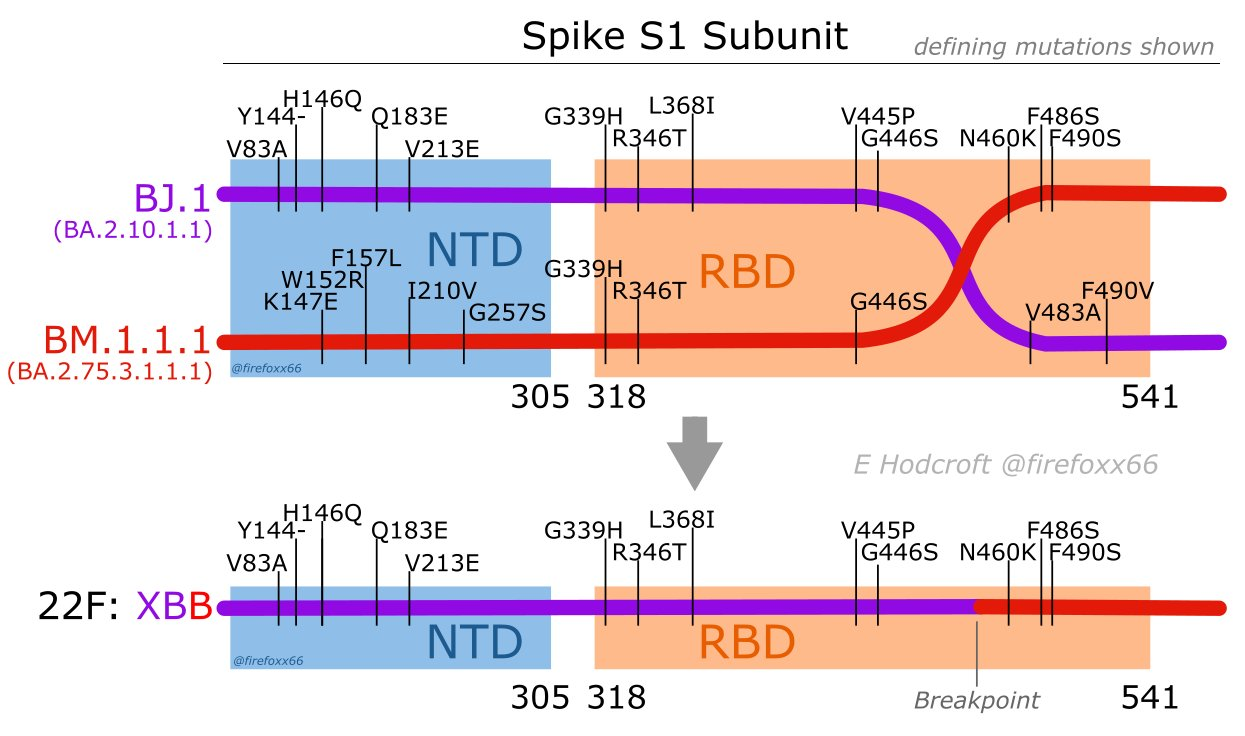
\includegraphics[width=0.7\textwidth,height=\textheight]{./Figures/recomb.jpeg}
\caption{Picture by Dr.~Emma Hodcraft at \url{https://twitter.com/firefoxx66/status/1587762412110974976/photo/1}}
\end{figure}

Notes:
NTD = N-terminal domain of the Spike protein (the ``beginning'' of the protein in that it is translated first)
RBD = Receptor binding domain of the Spike protein, which binds the ACE2 or other receptors

\hfill\break

\hypertarget{phylogenetic-trees}{%
\chapter{Phylogenetic Trees}\label{phylogenetic-trees}}

\hypertarget{sars-cov-2-variant-genomes-1}{%
\section{SARS-Cov-2 variant genomes}\label{sars-cov-2-variant-genomes-1}}

Now let's make a phylogenetic tree. We'll start with a web-based tool that can create phylogenetic trees.

Download mafft.sars-cov-2-variants.fasta file that you already made. It has the genome sequence of the four different SARS-Cov-2 variants in it. If it isn't completed yet, you can download mine at /home/jm/sars-variants/mafft.sars-cov-2-variants.fasta

Go to \url{https://www.ebi.ac.uk/Tools/phylogeny/simple_phylogeny/}

Upload the file and then click ``Submit''.

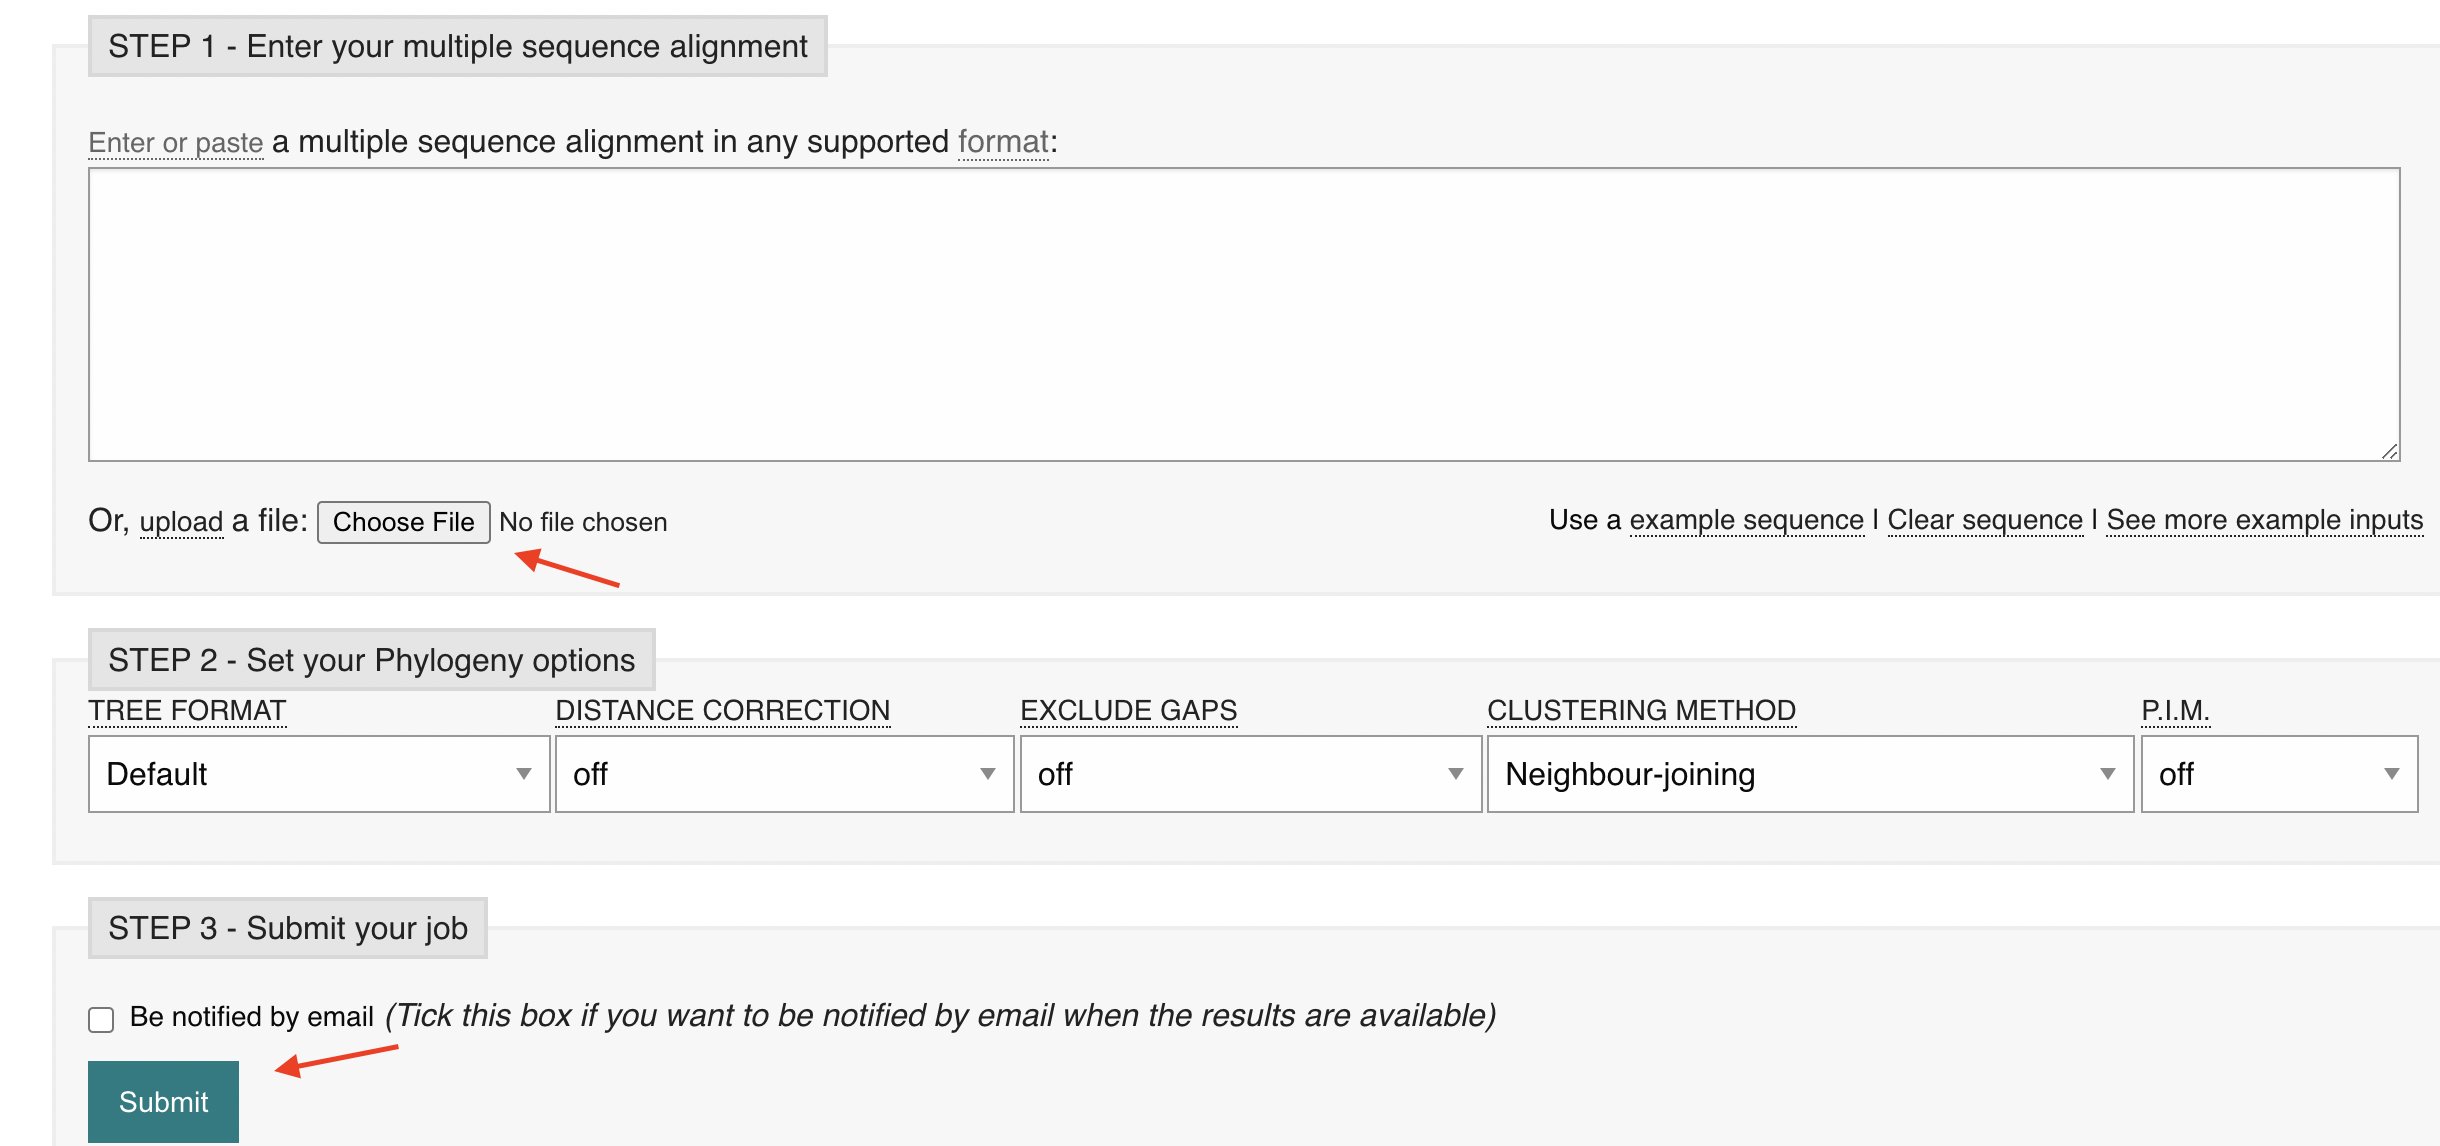
\includegraphics[width=0.7\textwidth,height=\textheight]{./Figures/SimplePhylogeny.png}

The tree should pop up. The cladogram just shows the groupings. If you choose real, it will change the branch lengths to the actual branch lengths.

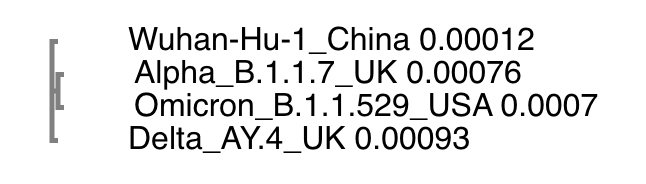
\includegraphics[width=0.7\textwidth,height=\textheight]{./Figures/real.png}

What do you notice about the tree?

Click for Possible Answers

\begin{verbatim}
The branch lengths are really small indicating that everything is closely related.

Alpha and Omicron are the most closely related, at least according to this tree.
\end{verbatim}

\hfill\break

The mafft.dns.spikeprot0702.fasta file is too large for this website so we need to learn how to do this on the command line. But we'll start off with the 4 variant sequences first.

Log into logrus and get into a screen. Navigate to your sars-variants folder. Do an ls to see what files are there.

Activate the environment. We'll use RAxML-ng to build the tree using the MAFFT files we already created. We'll use Wuhan-Hu-1 as the outgroup.

\begin{verbatim}
conda activate raxml-ng
\end{verbatim}

Create the tree.

\begin{verbatim}
raxml-ng --force model_lh_impr --outgroup Wuhan-Hu-1_China --all --msa mafft.sars-cov-2-variants.fasta --model GTR+G --tree pars{10} --bs-trees 100
\end{verbatim}

NOTE: The force param (--force model\_lh\_impr) makes it not quit if an optimized tree is only a smidge better than another tree. This is important for SARS-CoV-2 since we have a lot of similar or identical genome sequences that could be rearranged to give trees that have similar scores.

Take a look at the file that ends in .bestTree. This is a text version of a tree in Newick tree formt. The innermost parentheses show what is most closely related. Branch lengths are incorporated. We'll show you how to visualize this shortly.

Which are the 2 most closely related variants in this tree?

Which is the most distant?

Click for Answers

The Omicron and Alpha are most closely related.

The Wuhan-Hu-1 is the most distantly related.

((Delta\_AY.4\_UK:0.001021,(Omicron\_B.1.1.529\_USA:0.000703,Alpha\_B.1.1.7\_UK:0.000784):0.000100):0.000021,Wuhan-Hu-1\_China:0.000021)

\hypertarget{spike-protein}{%
\section{Spike Protein}\label{spike-protein}}

The mafft.dns.spikeprot0702.fasta file has spike protein sequences for Denmark, Norway, and Sweden that are already aligned.

First, we need to add in Wuhan-Hu-1 as our outgroup. We'll use an early isolate from the US that matched the Wuhan-Hu-1 that is present in the spike sequence file. Get isolate EPI\_ISL\_759860's header and sequence from spikeprot0702.fasta.gz and put it into a file called wuhanhu1.fasta.

Note: There are several accessions that start with EPI\_ISL\_759860 but we want \textbf{EPI\_ISL\_759860} not \textbf{EPI\_ISL\_759860}7, for instance, so search for `EPI\_ISL\_759860\textbar{}'

Click for Possible Answers

\begin{verbatim}
zgrep -A1 'EPI_ISL_759860|' spikeprot0702.fasta.gz > wuhanhu1.fasta
\end{verbatim}

\hfill\break

Now combine the dns.spikeprot0702.fasta (Denmark, Norway, Sweden spike sequences) and the wuhanhu1.fasta file you just made using the ``cat'' command. Put it in a file called dnsw.spikeprot0702.fasta

Click for Possible Answers

\begin{verbatim}
  cat wuhanhu1.fasta dns.spikeprot0702.fasta > dnsw.spikeprot0702.fasta
\end{verbatim}

\hfill\break

The Wuhan-Hu-1 header is really long and has a lot of special characters. Since we will be feeding that in on the command line, let's make it shorter.

Find the Wuhan-Hu-1 header.

Click for Possible Answers

\begin{verbatim}
  grep '>' Wuhan dnsw.spikeprot0702.fasta
\end{verbatim}

\hfill\break

Let's replace it so it just says Wuhan-Hu-1. Here is one way to do it.

NOTE: -i.bak tells sed to edit the file in place and make a backup of the original file, ading the .bak suffix.

\begin{verbatim}
sed -i.bak -e 's/^>.*\(Wuhan-Hu-1\).*/>\1/' dnsw.spikeprot0702.fasta
\end{verbatim}

Run a mulitple sequence alignment on the dnsw.spikeprot0702.fasta. This will take a will so if you need to, link to my file at /home/jm/sars-variants/mafft.dnsw.spikeprot0702.fasta (but make sure you name your file something different!). Use 8 threads.

NOTE: The number of threads is

\begin{verbatim}
--thread
\end{verbatim}

in MAFFT and

\begin{verbatim}
--threads
\end{verbatim}

in raxml-ng.

Click for Answer

\begin{verbatim}
mafft --thread 100 dnsw.spikeprot0702.fasta > mafft.dnsw.spikeprot0702.fasta
\end{verbatim}

\hfill\break

Now, create the tree. Use 8 threads.

Click for Answer

\begin{verbatim}
raxml-ng  --threads 8 --force model_lh_impr --outgroup Wuhan-Hu-1 --all --msa mafft.dnsw.spikeprot0702.fasta --model GTR+G --tree pars{10} --bs-trees 100
\end{verbatim}

\hfill\break

Now, create a tree for your 3 countries from the MSA you made earlier.

\hypertarget{visualizing-the-tree}{%
\section{Visualizing the tree}\label{visualizing-the-tree}}

Make sure you are in the sars-variants directory.

Click for Answer

\begin{verbatim}
cd ~/sars-variants
\end{verbatim}

\hfill\break

Activate the tree environment.

Click for Answer

\begin{verbatim}
conda activate tree

If it doesn't recognize the environment, try:
conda activate /home/condasw/miniconda3/envs/tree
\end{verbatim}

\hfill\break

Open up R.

\begin{verbatim}
R
\end{verbatim}

Load the following libraries. The treeio library is needed to read in the tree that we created. The ggtree library is an extension of ggplot2 for trees.

\begin{verbatim}
library(treeio)
library(ggtree)
library(ggplot2)
\end{verbatim}

Read in the tree for the SARS-CoV-2 variants that you created with RAxML-ng.

\begin{verbatim}
tr = read.tree("mafft.sars-cov-2-variants.fasta.raxml.bestTree")
\end{verbatim}

Create a PDF to put the tree in.

\begin{verbatim}
pdf("basic.tree.pdf")
\end{verbatim}

Now make the tree and release the PNG.

\begin{verbatim}
ggtree(tr)

dev.off()
\end{verbatim}

Use another terminal to download your PDF and look at it.

HINT: We'll be making several PDFs. I find it easier to set up my scp command to download all the PDFs (*pdf) in the sars-variants directory so I don't have to rewrite my command. They are small so redownloading previous PDFs isn't problematic.


\includegraphics[width=0.7\textwidth,height=\textheight]{./Figures/basic.tree.png}

Not much to look at and we definitely need some tip labels and a scale. So let's make some customizations.

Open up a PDF called ``labeled.tree.pdf''.

Click for Answers

\begin{verbatim}
pdf("labeled.tree.pdf")
\end{verbatim}

\hfill\break

ggtree follows ggplot2 grammar. We'll add some layers to add the tip labels and a scale bar. We'll also add a layer that will give us a theme that has an x axis scale running across the bottom as well, which we'll need in order to adjust the plot later on.

We are also going to put the tree plot into a variable so that we can add more layers to the variable later on, without having to keep adding the tip label, scale, and theme layers. The first command below puts the tree plot into the variable. The second command prints out the variable (and, hence, the tree plot).

\begin{verbatim}
mytree = ggtree(tr) + geom_tiplab() + geom_treescale() + theme_tree2()

mytree

dev.off()
\end{verbatim}

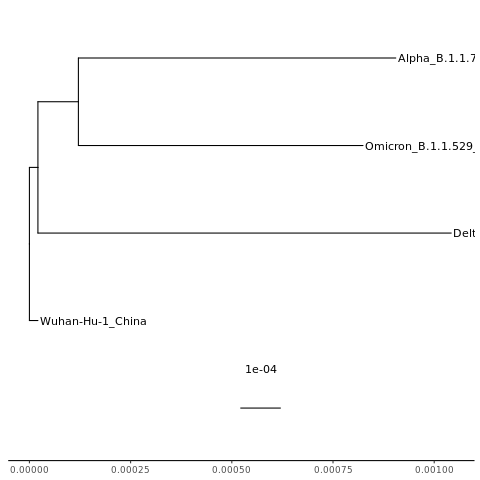
\includegraphics[width=0.5\textwidth,height=\textheight]{./Figures/labeled.tree.png}

NOTE: The scale/branch lengths are a nucleotide distance. In other words, 1e-04 means one nucleotide change in every 10,000 nucleotides.

Some of our labels got cut off. We need to change how far the x axis goes. Looking at the plot we just made, the tips of the tree go out to about 0.001. So let's change the x axis to go a little further (0.002), which means the bars won't get quite so far to the right and the text will have more space.

Open up a PDF called ``scaled.tree.pdf''.

Click for Answers

\begin{verbatim}
pdf("scaled.tree.pdf")
\end{verbatim}

\hfill\break

Create the tree then close the PNG. We can start with the mytree variable that we made above. We'll add on a layer from ggplot2 called xlim, giving it a range from 0 to 0.002. We'll also add a title layer.

\begin{verbatim}
mytree2 = mytree + ggplot2::xlim(0, 0.002) + ggtitle("SARS-CoV-2 Variants")

mytree2

dev.off()
\end{verbatim}

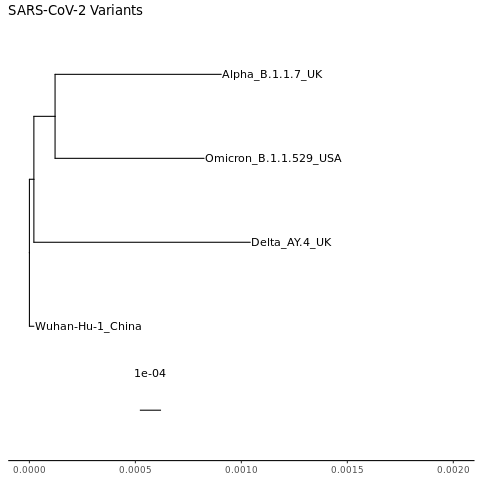
\includegraphics[width=0.5\textwidth,height=\textheight]{./Figures/scaled.tree.png}

That's better. Notice that the farthest tips still end around 0.001.

Now, let's make the tip text labels larger and color the tip points.

Open up a PDF called ``tip.tree.pdf''.

Click for Answer

\begin{verbatim}
png("tip.tree.png")
\end{verbatim}

\hfill\break

We'll start from scratch since the variables we have created already have a geom\_tiplab so will end up with 2 different labels of 2 different sizes. As we make the tip point bigger, it will overlap the tip label so we'll shift the tip label to the right using hjust (horizontal justification).

\begin{verbatim}
mytree3 = ggtree(tr) + geom_treescale() + theme_tree2() + ggplot2::xlim(0, 0.002) + ggtitle("SARS-CoV-2 Variants") + geom_tiplab(size=7, hjust = -0.1) + geom_tippoint(color="blue",size=8)

mytree3

dev.off()
\end{verbatim}

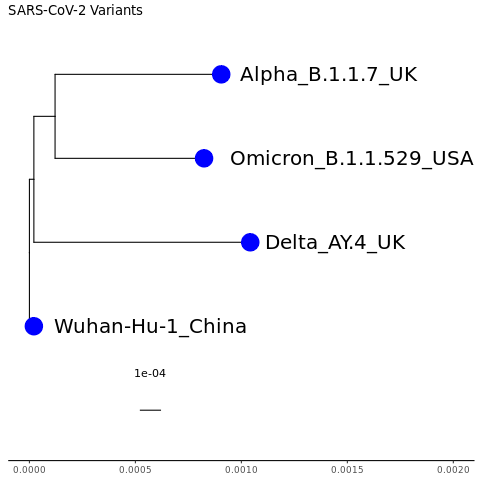
\includegraphics[width=0.35\textwidth,height=\textheight]{./Figures/tip.tree.png}

If you wanted to also color the tip label text blue, how do you think you would you do it?

Click for Answer

\begin{verbatim}
ggtree(tr) + geom_treescale() + theme_tree2() + ggplot2::xlim(0, 0.002) + ggtitle("SARS-CoV-2 Variants") + geom_tiplab(size=7, hjust = -0.1, color="blue") + geom_tippoint(color="blue",size=8)
\end{verbatim}

\hfill\break

Note: There is also a geom\_nodepoint variable that you can use to put dots or other shapes on the internal nodes to highlight a clade. To find out more about customizing phylogenetic trees, see \url{https://yulab-smu.top/treedata-book/index.html}.

We can also color the nodes by another variable. We'll color by country.

We need to make a table linking each sequence name to its country. Go into a different window in your screen (ctrl-a + c : creates a new one; ctrl-a space : moves you through different screen windows). In your sars-variants directory, look at your sars-cov-2-variants.fasta file. We will grab the header lines from the file and parse it into a table with sequence\_name and country. See if you can figure out what each piece of the command below does.

\begin{verbatim}
grep '>' sars-cov-2-variants.fasta | sed 's/>//' | awk '{print $1 "\t" $1}' | sed 's/\t.*_/\t/' > sars-cov-2-variants.countries.txt
\end{verbatim}

Take a look at the sars-cov-2-variants.countries.txt file.

Click for Answer

\begin{verbatim}
cat sars-cov-2-variants.countries.txt

or 

more sars-cov-2-variants.countries.txt

or

less sars-cov-2-variants.countries.txt

or

head sars-cov-2-variants.countries.txt

etc
\end{verbatim}

\hfill\break

Now go back to the screen window that has R open.

Read in the sars-cov-2-variants.countries.txt file that we just created and give it some column names. Then take a look at it.

\begin{verbatim}
countrydf = read.table("sars-cov-2-variants.countries.txt", header=FALSE)

colnames(countrydf) = c("SequenceVariant", "Country")

head(countrydf)
\end{verbatim}

Open up a PDF called ``country.tree.pdf''.

Click for Answer

\begin{verbatim}
pdf("country.tree.pdf")
\end{verbatim}

\hfill\break

We have to append the data frame with the country info to the tree and then we can use the country column to color the tip points. We'll also add a legend layer. Note that you need to put the color in ``aes''. Otherwise, it can't find the country column.

\begin{verbatim}

mytree4 = mytree3 %<+% countrydf + geom_tippoint(aes(color=Country), size=8) + theme(legend.position=c(0.85,0.15))

mytree4

dev.off()
\end{verbatim}

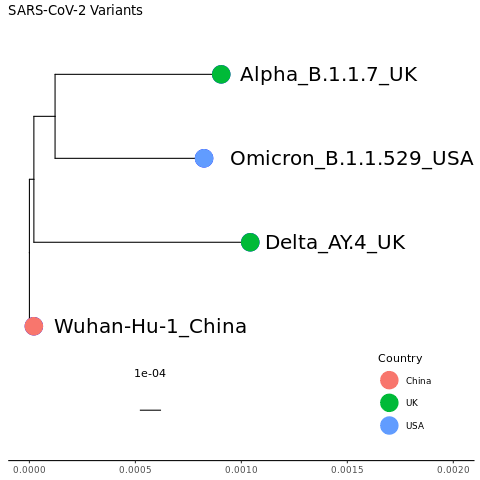
\includegraphics[width=0.35\textwidth,height=\textheight]{./Figures/country.tree.png}

We can also add in the multiple sequence alignment next to the tree. Read in the mafft multiple sequence alignment file.

\begin{verbatim}
msafa = treeio::read.fasta("mafft.sars-cov-2-variants.fasta", type="NT")
\end{verbatim}

Now, we'll use msaplot from ggtree to add the msa.

\begin{verbatim}
pdf("msa.tree.pdf")

msaplot(mytree4, fasta=msafa, width=2)

dev.off()
\end{verbatim}

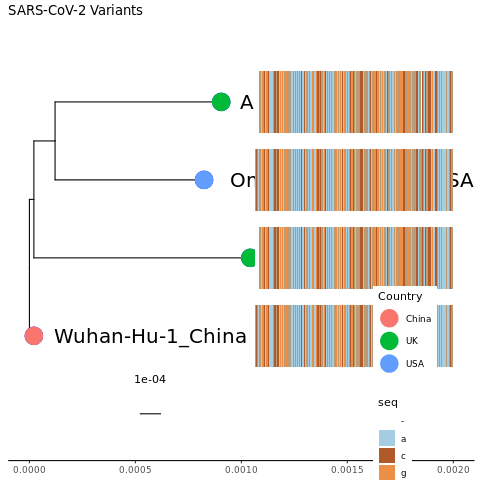
\includegraphics[width=0.35\textwidth,height=\textheight]{./Figures/msa.tree.png}

OK, cool! We have just squeezed the nearly 30,000 nucleotide genome onto the plot. Obviously, there are a few problems. We have overwritten our labels and the sequence in the MSA is so squeezed that it is hard to see it in general or to pick out any differences. We now have a second legend that tells the colors of the nucleotides and neither legend is in a good place.

We need to shift the MSA seqence to the right (hjust isn't recognized by msaplot but there is an ``offset'' command).

We should tell msaplot the relative width of the MSA compared to the tree (``width'' command).

We need to make the PDF wider. We'll change it from its default of 8.5 inches to 85 inches.

We need to make room for the legends and adjust where they are. To do this last one, we'll need to remake our plot in mytree4. To keep things seperate, we'll put it into mytree5 rather than overwriting mytree4.

Let's also get rid of the scale across the x axis, now that it has served its purpose. That will require starting from scratch. We also need to expand the x axis coordinates to be able to fit the MSA.

\begin{verbatim}
mytree5 = ggtree(tr)  %<+% countrydf + geom_treescale() + ggplot2::xlim(0, 0.02) + ggtitle("SARS-CoV-2 Variants") + geom_tiplab(size=7, hjust = -0.1) + geom_tippoint(aes(color=Country), size=8) + theme(legend.position=c(0.02,0.6)) + ggplot2::xlim(0, 0.02) + ggplot2::ylim(-2, 5)

pdf("msa.big.tree.pdf", width=85)

msaplot(mytree5, fasta=msafa, width=15, offset=0.0008)

dev.off()
\end{verbatim}

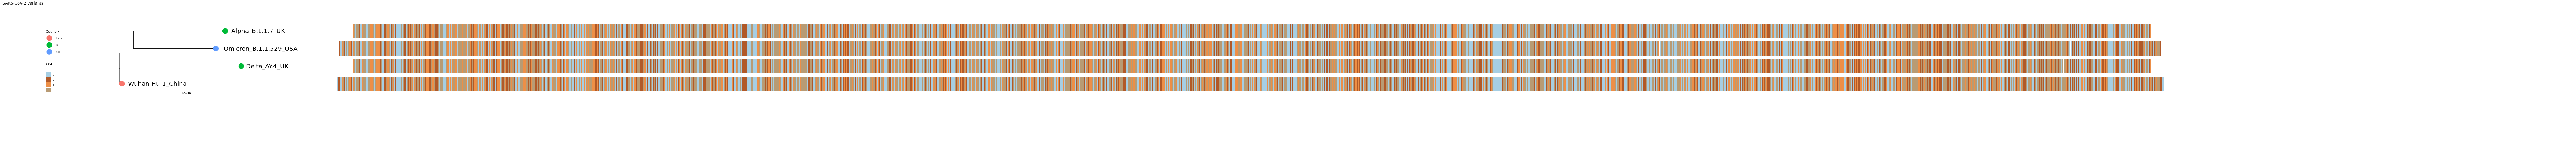
\includegraphics[width=1\textwidth,height=\textheight]{./Figures/msa.big.tree.png}

Looks great! Might need to zoom in too look at it more closely.

But that's a lot of sequence to squeeze onto there. Let's just show the spike nucleotide sequence. We can still use the mytree5 variable since the change in the MSA will happen in msaplot. Remember that the spike protein coordinates in Wuhan are 21563-25384.

NOTE: Even though we will just be showing the spike sequence in the MSA, the tree itself was built considering the entire SARS-CoV-2 genome.

\begin{verbatim}
pdf("msa.spike.msa.tree.pdf", width=85)

msaplot(mytree5, fasta=msafa, width=15, offset=0.0008, window=c(21563,25384))

dev.off()
\end{verbatim}

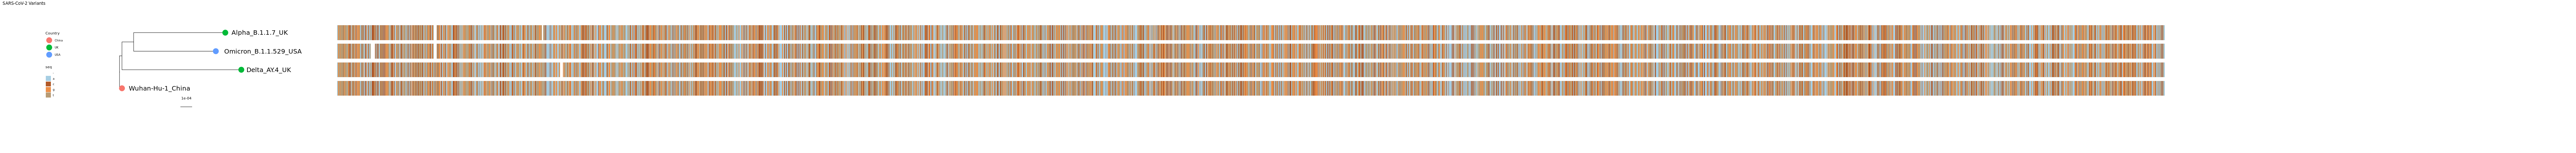
\includegraphics[width=1\textwidth,height=\textheight]{./Figures/msa.spike.msa.tree.png}

As we have already learned there are no insertions in these variants relative to Wuhan (thought there are in other variants). If there were, the coordinates in the MSA for spike would shift slightly. Let's double-check that there is a start codon at the beginning and a stop codon at the end. Zoom in to see the first and last 3 nucleotides. The link below takes you to a codon wheel so you can see what the codons you find code for.

\url{https://www.sigmaaldrich.com/US/en/technical-documents/technical-article/genomics/sequencing/amino-acid-codon-wheel}

Click for Answer

\begin{verbatim}
The starting codon is ATG which is the start codon.
The ending codon is TAA which is a stop codon.
\end{verbatim}

\hfill\break

How many deletions relative to Wuhan do you see for Alpha, Delta, and Omicron?

Click for Answer

\begin{verbatim}
Deletions
Alpha   2
Delta   1
Omicron   2
\end{verbatim}

\hfill\break

Let's make a tree for the Denmark, Norway, Sweden Arcturus sequences color coded by country. We'll rely on the color for country and not worry about the tip labels. We'll just focus on the tree and not worry about the MSA. Try it yourself before looking at the answer.

If you don't have a tree made, link to mine (/home/jm/gisaid\_genomes/mafft.dns.arcturus.fasta).

These are the steps you'll need to take:

\begin{enumerate}
\def\labelenumi{\arabic{enumi}.}
\tightlist
\item
  Switch to the gisaid\_genome directory in R.
\item
  Create a file that links each sequence to the country it came from in linux.
\end{enumerate}

HINT: You can use sed as we did for the SARS-CoV-2 variants, but here is an easier way. The ``paste'' command pastes columns from different files together.

\begin{verbatim}
# Example header
# >hCoV-19/Sweden/AB-502030/2023|EPI_ISL_17850020|2023-06-16

grep '>' mafft.dns.arcturus.fasta | sed 's/>//' > temp1.txt
cut -f 2 -d '/' temp1.txt > temp2.txt
paste temp1.txt temp2.txt > dns.arc.country.txt
rm temp*
\end{verbatim}

\begin{enumerate}
\def\labelenumi{\arabic{enumi}.}
\setcounter{enumi}{2}
\tightlist
\item
  Create a tree in linux.
\end{enumerate}

The rest of the steps are in R.

\begin{enumerate}
\def\labelenumi{\arabic{enumi}.}
\setcounter{enumi}{3}
\item
  Read in the country file and column headers.
\item
  Read in the tree file.
\item
  Plot your tree.
\end{enumerate}

Click for Answers

\begin{verbatim}
1. setwd("/home/jm/gisaid_genomes/")

2. grep '>' mafft.dns.arcturus.fasta | sed 's/>//' > temp1.txt
cut -f 2 -d '/' temp1.txt > temp2.txt
paste temp1.txt temp2.txt > dns.arc.country.txt
rm temp*

3. raxml-ng --force model_lh_impr --all --msa mafft.dns.arcturus.fasta --model GTR+G --tree pars{10} --bs-trees 100

4. dnscountrydf = read.table("dns.arc.country.txt", header=FALSE)

colnames(dnscountrydf) = c("SequenceVariant", "Country")

5. dnsarctr = read.tree("mafft.dns.arcturus.fasta.raxml.bestTree")

6. pdf("dns.arc.pdf", height=15, width=10)

dnsarc = ggtree(dnsarctr)  %<+% dnscountrydf + geom_treescale() + ggtitle("Denmark, Norway, and Sweden Arcturus Sequences") + geom_tippoint(aes(color=Country), size=1) + theme(legend.position=c(0.04,0.9))

dnsarc

dev.off()
\end{verbatim}

\hfill\break

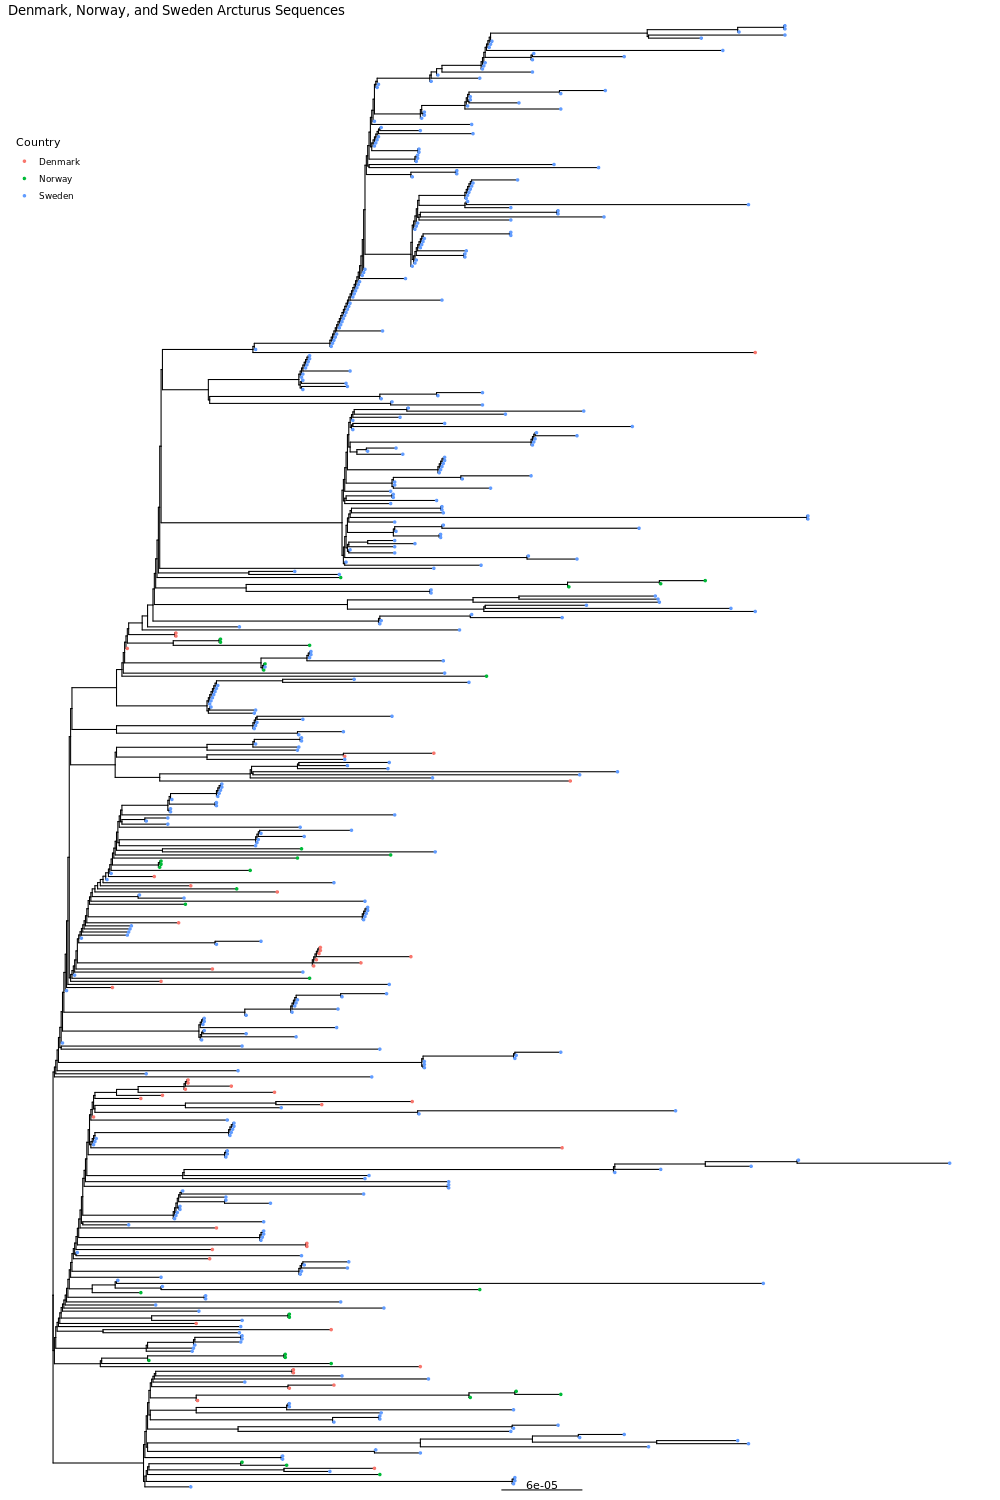
\includegraphics[width=0.5\textwidth,height=\textheight]{./Figures/dns.arc.png}

Now try to create a phylogenetic tree with your arcturus 3 country data. Think about these questions before we share the plots with each other.

Do the sequences from each country form their own clade?

Does it look like the sequences are evolving separately within each country?

Are any clades specific to one country or absent from one country?

Keep in mind that it is hard to compare numbers directly across countries because each country sequenced a different number/percentage of cases. But do you see any interesting patterns such as a high percentage of a country's sequences being in the beginning or later in the pandemic, and do these patterns match what you know about the course of the pandemic in these countries?

\hypertarget{dotplots}{%
\chapter{Dotplots}\label{dotplots}}

We are going to make dotplots, which is a way to line up two genomes and see high level structural differences between them (large insertions and deletions, translocations, inversions, etc). Single nucleotide changes (SNPs) and small indels are ignored at this level.

\hypertarget{sars-cov-2}{%
\section{SARS-CoV-2}\label{sars-cov-2}}

We'll start with SARS-CoV-2.

Make a directory called ``dotplots'' and navigate into it.

Soft-link to the data (/home/jm/sarsdata/dotplotgenomes/*.fa).

Activate the mm2 environment. This will allow us to run minimap2, an aligner (like BLAST) that will very quickly give us approximate genome-wide alignments.

Click for Possible Answers

\begin{verbatim}
mkdir ~/dotplots

cd dotplots

ln -s /home/jm/sarsdata/dotplotgenomes/*.fa .

conda activate mm2
\end{verbatim}

\hfill\break

Look at the man page to figure out what the following parameters mean:
-x asm20
-o
-c (we'll use this in a bit)

Run minimap2 putting it into an out put file called SARS-CoV-2xSARS-CoV.paf.

\begin{verbatim}
minimap2 -x asm20 -o SARS-CoV-2xSARS-CoV.paf SARS-CoV.fa SARS-CoV-2.fa
\end{verbatim}

Take a look at the file. Go to the following website to learn about PAF (Pairwise mApping Format) format (click on ``Output Format''). Work through the documentation on the website as a group to figure out what each part of it means.

\url{https://lh3.github.io/minimap2/minimap2.html}

How many alignments did we get across the genome?

Click for Possible Answers

\begin{verbatim}
Only 1.

It's easy to open the file and count the 1 alignment but if we had a lot of alignments, we would want a better way to do that:

wc -l SARS-CoV-2xSARS-CoV.paf
\end{verbatim}

\hfill\break

There are parameters that will allow minimap2 to convert those approximate alignments to nucleotide-level alignments but it doesn't often change anything on dotplot level. But let's run it and see. It prints out a CIGAR string, which is something that you'll see a lot in alignment files and is good to unerstand. We'll use the -c parameter.

\begin{verbatim}
minimap2 -c -x asm20 -o SARS-CoV-2xSARS-CoV.cigar.paf SARS-CoV.fa SARS-CoV-2.fa
\end{verbatim}

Many alignments are printed out in SAM format or the compressed version of SAM called BAM. Go to the sam documentation:
\url{https://samtools.github.io/hts-specs/SAMv1.pdf} \#6

How is SAM different than PAF? This document also has information on the CIGAR string. See if you can figure out what the CIGAR string in our PAF file is telling us.

OK. Now let's plot it.

Go to another window in your screen and activate the visualization environment.

\begin{verbatim}
ctrl-a+c to create a new screen or ctrl-a+space to navigate to the next screen

conda activate visualization
\end{verbatim}

We'll use dotplotly which uses R and the ggplot2 and plotly libraries to make both static and interactive dotplots.

Find out what the parameters for dotplotly are. There is no help function so just google dotplotly. Pay attention especially to:
-i
-o
-m
-q
-l
-p

We need to change the -q parameter from the default. Why?

Run dotplotly.

\begin{verbatim}
/home/jm/sw/dotPlotly-master/pafCoordsDotPlotly.R -i SARS-CoV-2xSARS-CoV.paf -o SARS-CoV-2xSARS-CoV -m 1000 -q 2000 -l -p 12
\end{verbatim}

Ignore the ``Error in htmlwidgets::saveWidget''. We don't have that library installed so our html isn't all in one document but requires us to copy over the folder. Copy over the png, html and the folder to your desktop computer using scp. When you copy over the folder, you need to use the -r (recursive) parameter.

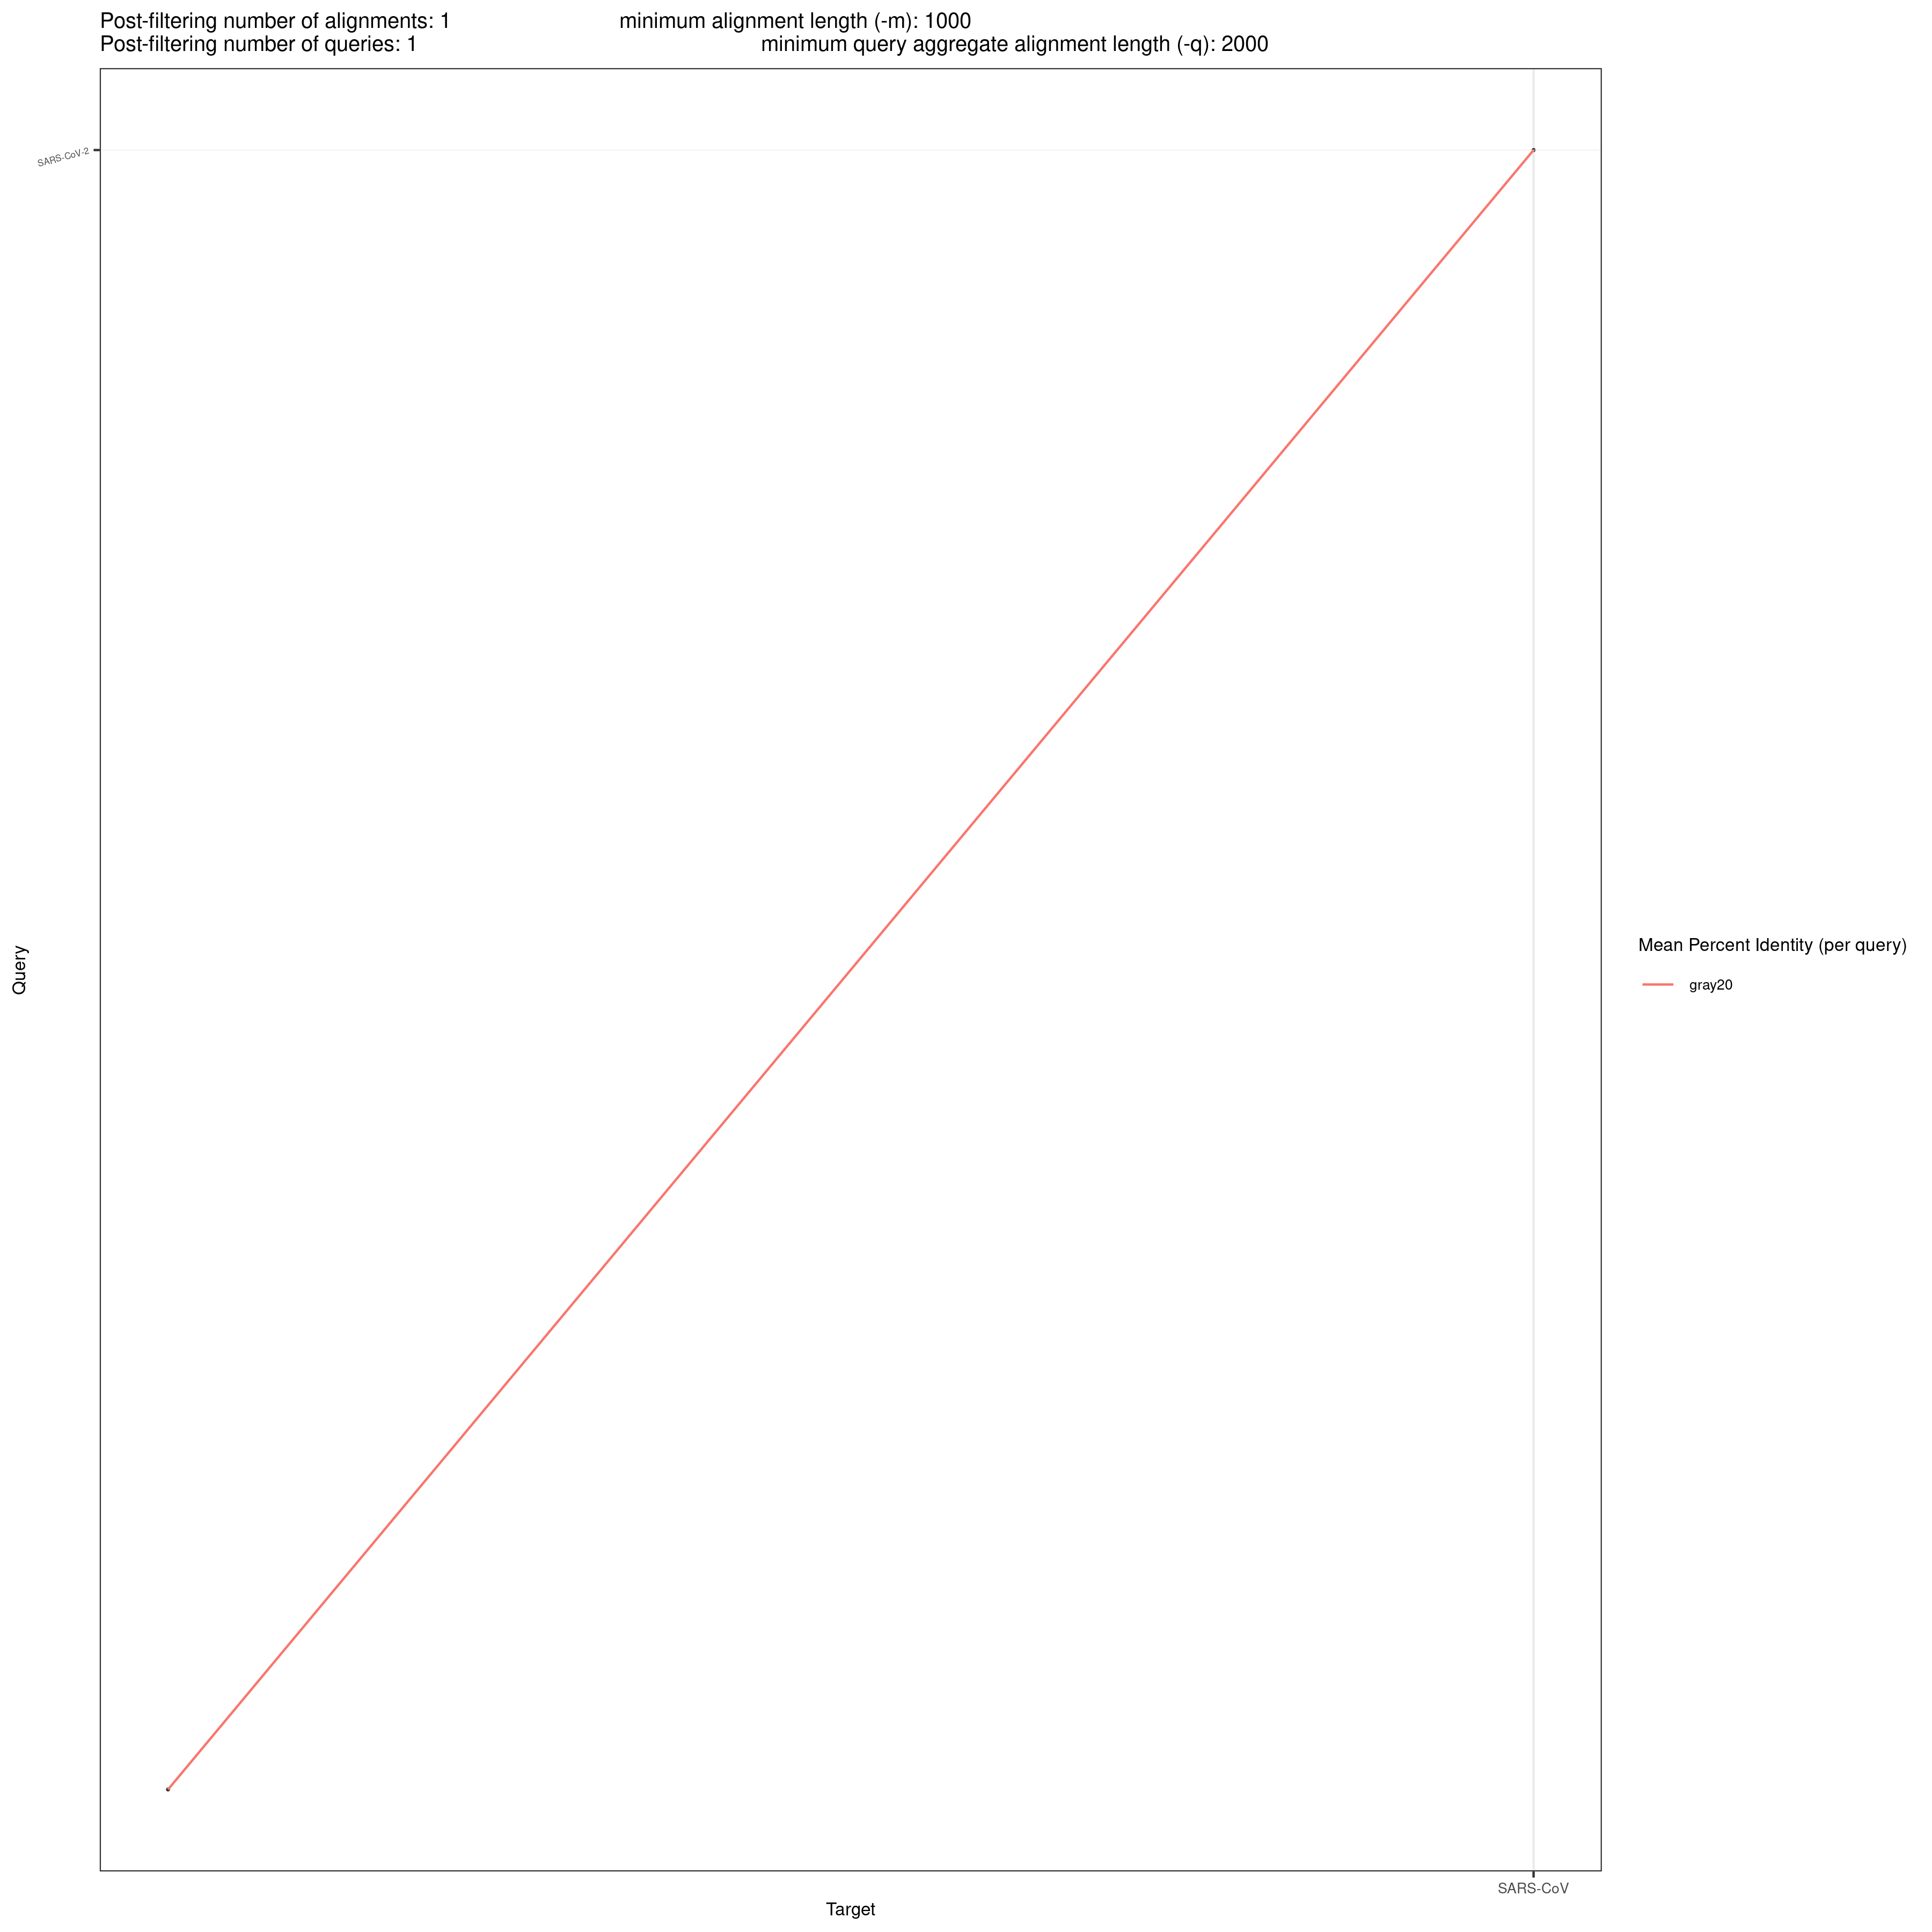
\includegraphics[width=0.7\textwidth,height=\textheight]{./Figures/SARS-CoV-2xSARS-CoV.png}

Open the PNG file. The single diagonal line means that they line up across there genomes (expect a bit at the beginning in the bottom left). At a high level structural view, SARs-CoV (the original SARS) and SARs-CoV-2 are very similar.

Now open the HTML file (make sure the folder is in the same directory). Play around with the controls on the top right and figure out what they do. Did you find how to activate the labels upon hovering?

Now run it on the PAF file with the CIGAR string and see if you get anything different.

\begin{verbatim}
/home/jm/sw/dotPlotly-master/pafCoordsDotPlotly.R -i SARS-CoV-2xSARS-CoV.cigar.paf -o SARS-CoV-2xSARS-CoV.cigar -m 1000 -q 2000 -l -p 12
\end{verbatim}

\hfill\break

How many alignments did it filter out?

It filtered out 1 alignment to keep 3 of the 4 alignments

\hfill\break

The filtered alignment was probably too short. How long are each of the alignments?

Hint: You can use the start and end of the alignments in the query that are in columns 3 and 4. Use awk and subtract those columns.

awk `\{print \$4-\$3+1\}' SARS-CoV-2xSARS-CoV.cigar.paf

Alignment lengths:
11596
1639
3940
832

\hfill\break

Since we set the minimum query length at 1000 (-m 1000), the shortest alignment got filtered out).

Rerun the dotplot to keep that alignment.

\begin{verbatim}
/home/jm/sw/dotPlotly-master/pafCoordsDotPlotly.R -i SARS-CoV-2xSARS-CoV.cigar.paf -o SARS-CoV-2xSARS-CoV.cigar -m 800 -q 2000 -l -p 12
\end{verbatim}

\hfill\break

Download your files and take a look at the plot.

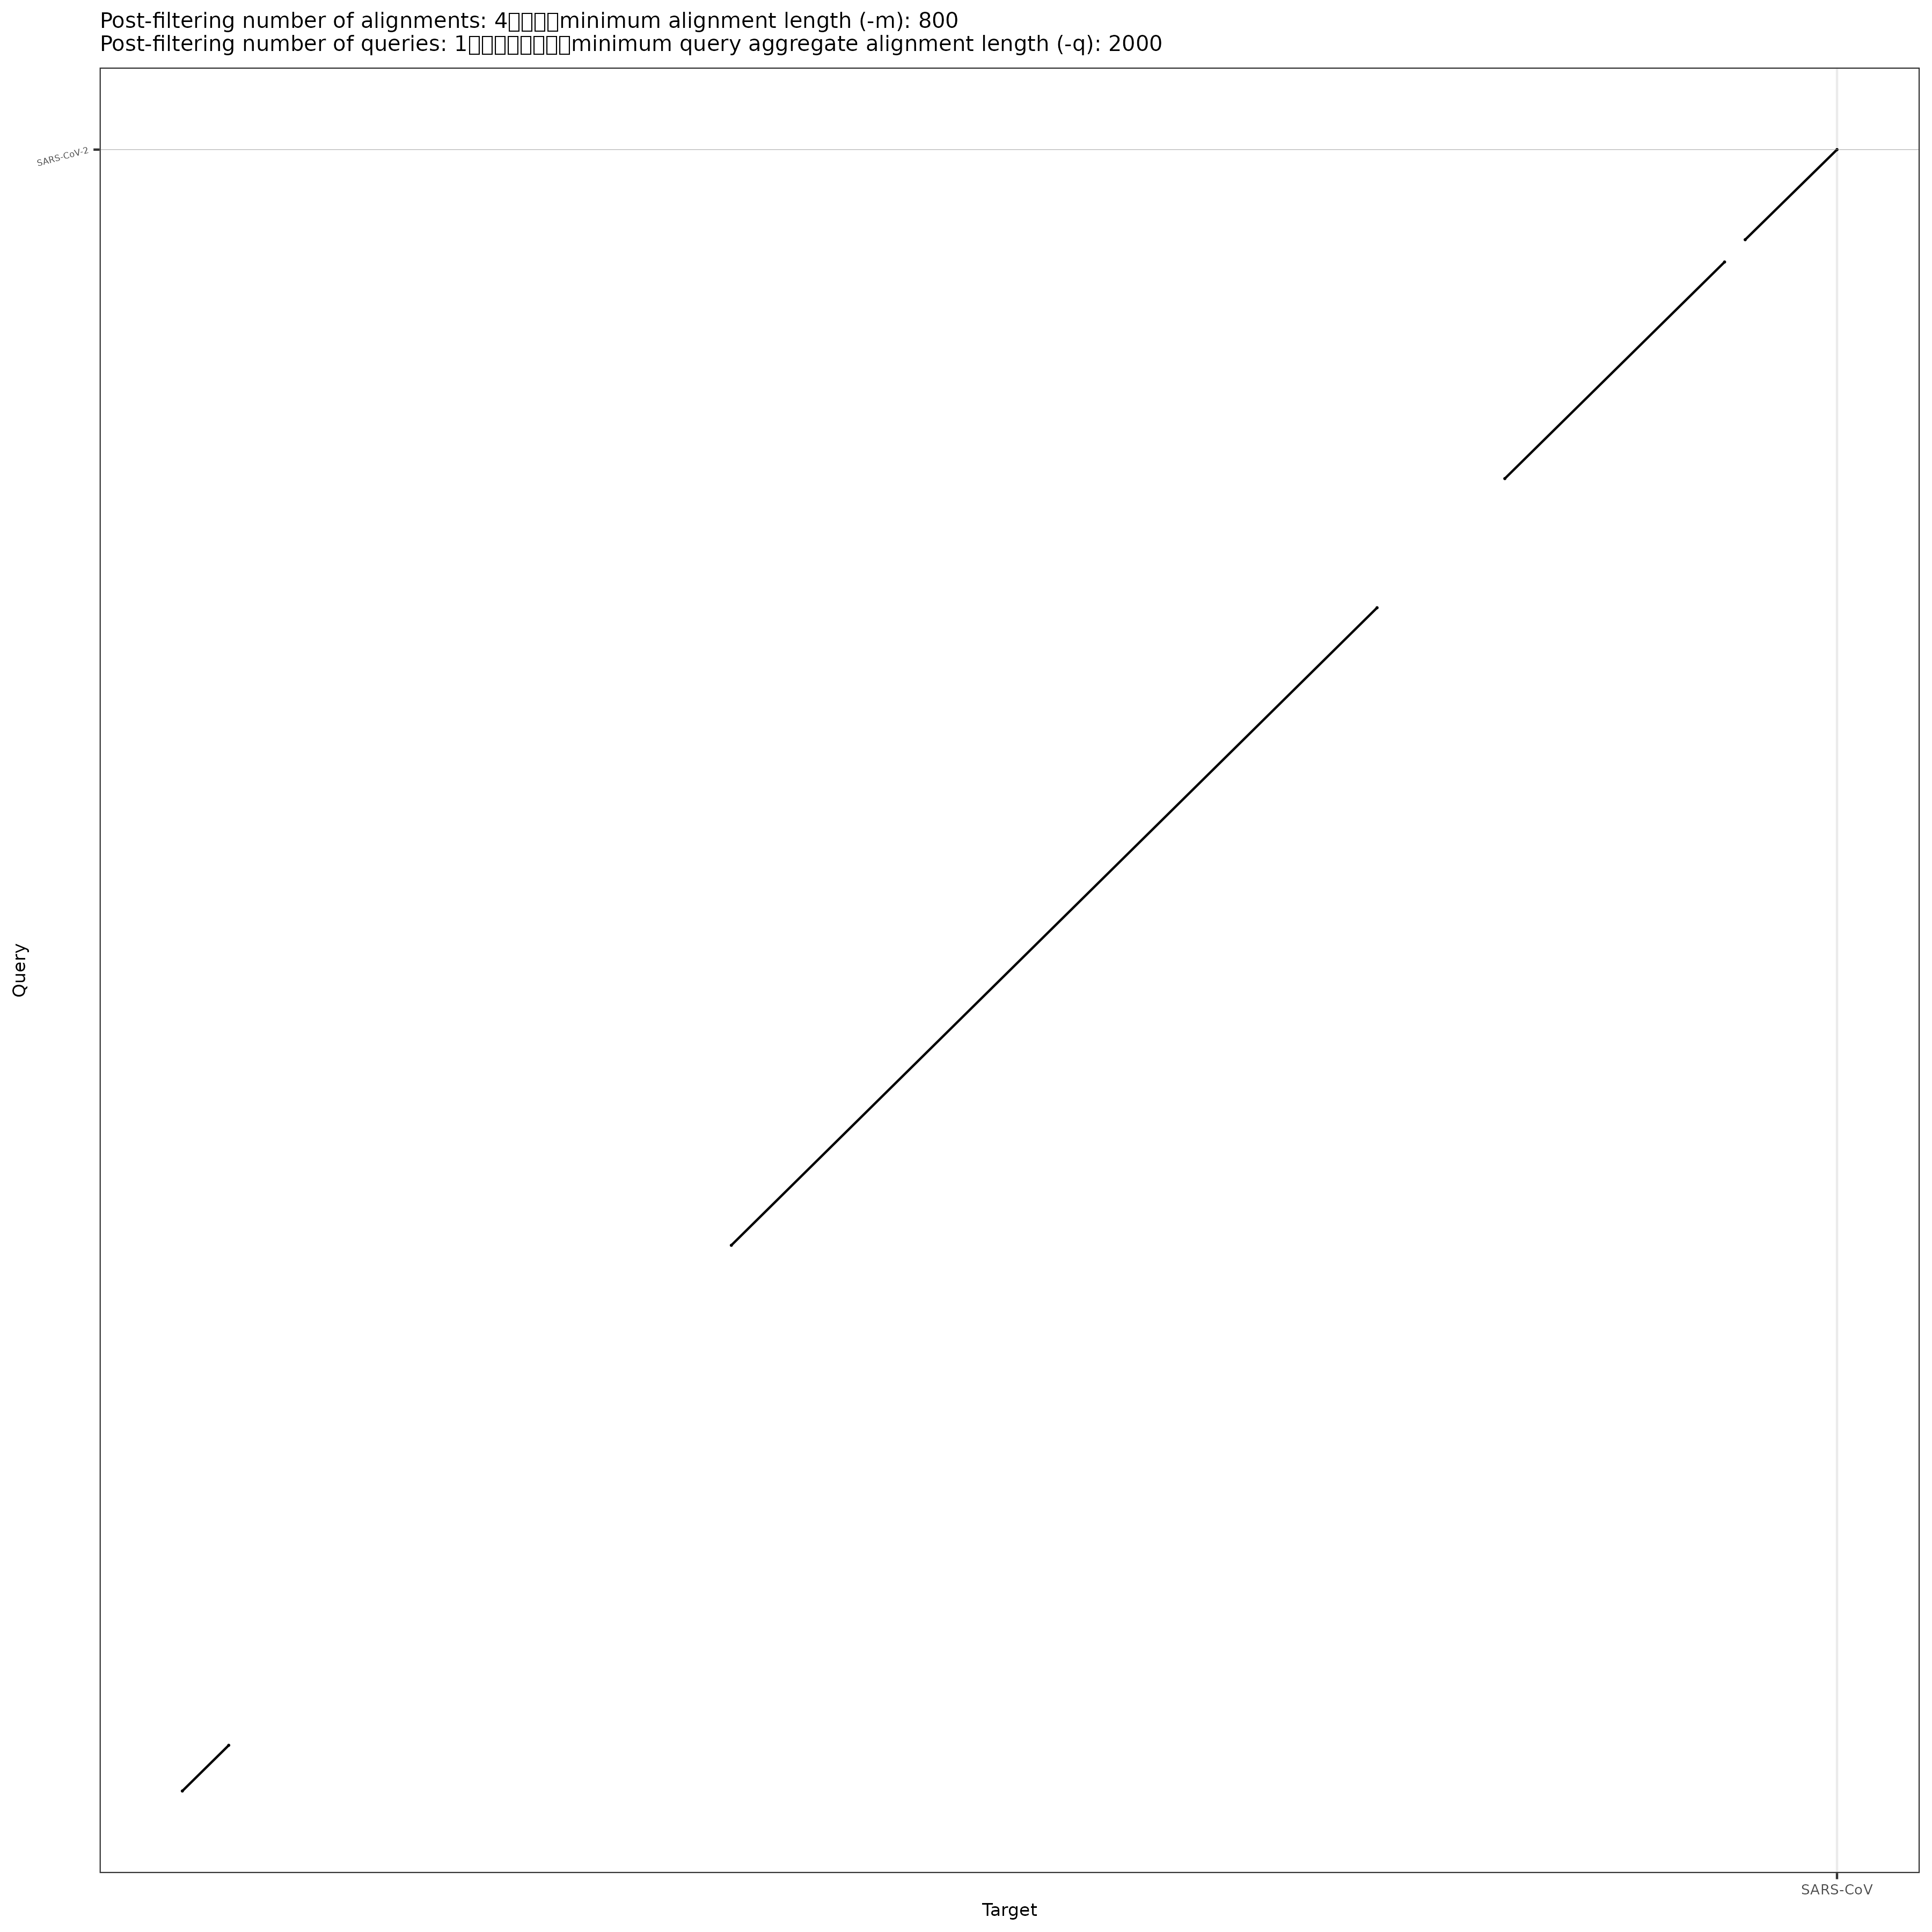
\includegraphics[width=0.45\textwidth,height=\textheight]{./Figures/SARS-CoV-2xSARS-CoV.cigar.png}

That is probably a more realistic representation of the relationship between the SARS-CoV-2 and SARS-CoV genomes.

\hypertarget{yersinia}{%
\section{Yersinia}\label{yersinia}}

Let's look at Yersinia. We'll compare Yersinia pestis to Yesinia enterocolitica. They are both pathogens. Look up what diseases/symptoms both of them cause.

How many sequences do each have? You linked to the files earlier. Do an ``ls'' to figure out the file names.

Click for Possible Answers

\begin{verbatim}
grep -c '>' Y*.fa
\end{verbatim}

\hfill\break

Plasmids often have virulence factors on them (the genes that make them pathogenic). Plasmids can be passed between bacteria of different species and so are often less related than the genomic chromosome is. In this case the genomic chromosome is circular.

Here are the lengths of each oof the chromosomes.

Y. enterocolitica
chr 4540172\\
plasmid1 5350\\
plasmid2 3300

Y. pestis
chr 4553770\\
plasmid1 96210\\
plasmid2 8431

Go back to your screen window with the mm2 environment.

Run minimap2 using nucleotide-level alignment to produce CIGAR strings.

\begin{verbatim}
minimap2 -c -x asm20 -o YexYp.cigar.paf Ypestis.fa Yenterocolitica.fa
\end{verbatim}

Run dotplotly with a minimum alignment length of 1000

\begin{verbatim}
/home/jm/sw/dotPlotly-master/pafCoordsDotPlotly.R -i YexYp.cigar.paf -o YexYp -m 1000 -q 2000 -l -p 12
\end{verbatim}

How many alignments did it filter out?

It filtered out 46 alignment to keep 428 of the 474 alignments

\hfill\break

Go ahead and download it and take a look.

This is much more rearranged than the SARS plots. See if you can see any patterns. Do the 2 genomes share any sequence in common? What about the ordering? Is anything inverted between the two genomes? Is anything duplicated? What can you tell about the plasmids?

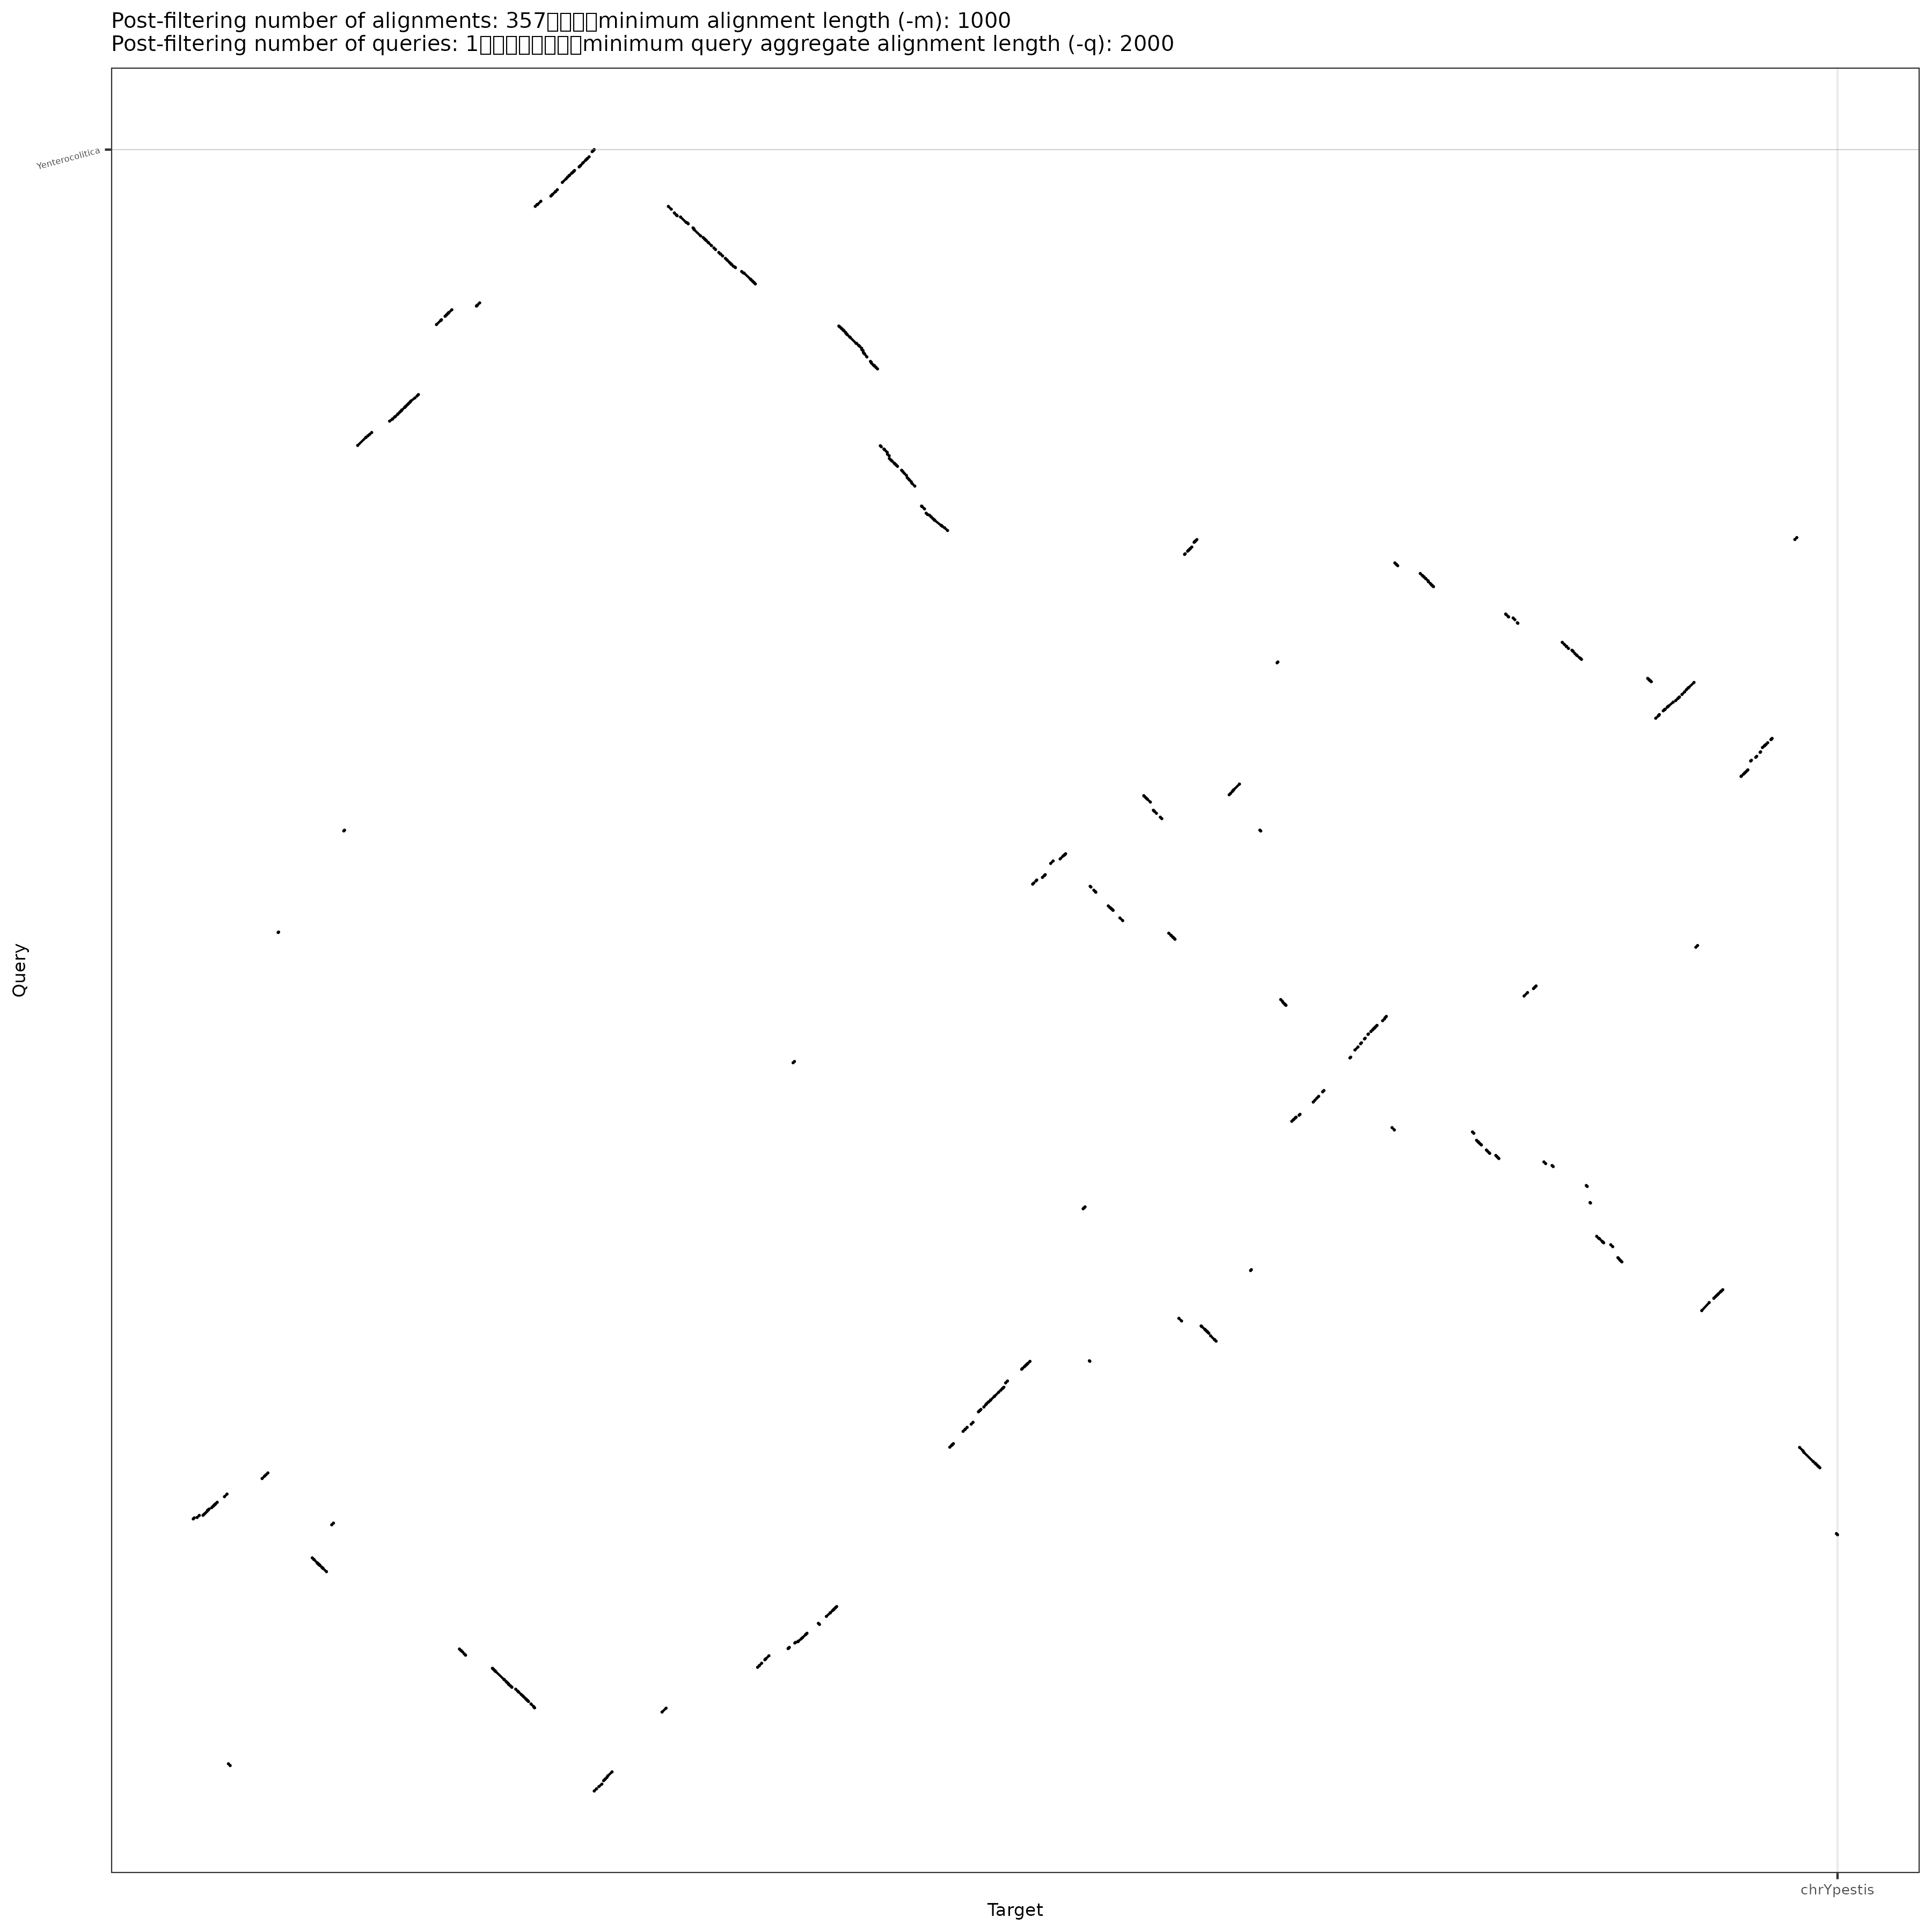
\includegraphics[width=0.45\textwidth,height=\textheight]{./Figures/YexYp.png}

\hypertarget{ancient-pandemic}{%
\chapter{Ancient Pandemic}\label{ancient-pandemic}}

Scientists recently obtained and sequence DNA from 3 individuals who died about 4,000 years ago. They do this by drilling into the teeth and obtain a sample of dental plaque. The plaque is known to preserve DNA from pathogens. They started off with 34 individuals (30 from the southern site and 4 from the northern site, both described below) and then focused on pathogens recovered from 3 of them.

They focused on two indiviuals from a mass burial site in Charterhouse Warren, Somerset (southern England). This type of mass burial was unusual in the region and, therefore, might represent an event where a lot of people died, such as an epidemic or a war. Signs of fatal trauma were seen in some individuals buried at the site suggesting that the people in this gravesite were killed in all together. Both were children around ages 10 and 12 (plus or minus 3 years). They used radiocarbon dating of the mandible bone in one individual, dating the grave to \textasciitilde4000 years ago.

A third individual was buried under a ring cairn monument in Levens, Cumbria (northern England). This person was buried on their own. This individual has also been dated to \textasciitilde4000 years ago. This individual is a female who is 35-45 years and has pottery shards alongside her as well as planks, which might have been a wooden coffin that she was crouched in.

We'll start with data from one of the individuals at the southern site (C10098). The scientists sequenced all the DNA in the sample, then they enriched for the pathogen DNA and sequenced again. We'll use the enriched sample.

Log onto logrus, enter a screen, create a directory called ancientpathogen in your home directory and navigate into it.

\begin{verbatim}
mkdir ~/ancientpathogen
cd ~/ancientpathogen
\end{verbatim}

Link to the data. You can find it in /home/jm/nise-data/*q.gz. This is single end Illumina data. What does that mean?

\begin{verbatim}
ln -s /home/jm/nise-data/*q.gz .
\end{verbatim}

Take a look at the filenames. Look at the file with ERR11262426 in the filename. This is a sample called C10098 from southern England. Note what the headers start with. Go back to the linux section if you need a refresher on fastq format.

\begin{verbatim}
ls -l

zcat ERR11262426.fastq.gz | head
\end{verbatim}

How many reads are there?

\begin{verbatim}
zgrep -c "^@ERR" /home/jm/nise-data/ERR11262426.fastq.gz
\end{verbatim}

Let's run FastQC, a tool that runs quality control metrics on fastq files. We can leave the fastq files zipped.

activate the fastQC environment. If conda can't find it, use:

\begin{verbatim}
conda activate /home/condasw/miniconda3/envs/fastQC
\end{verbatim}

Make a directory called ``fastqc'' in your current directory. This will be our output directory.

\begin{verbatim}
mkdir fastqc
\end{verbatim}

Now run FastQC.

\begin{verbatim}
fastqc -o fastqc ERR11262426.fastq.gz
\end{verbatim}

Copy the html and zip files over to your desktop, then unzip the .zip file and open up the html file. Go through it as a group.

Let's look to see if there are any sequences from bacterial species included among the human sequences. I grabbed all of the complete bacterial genomes from Genbank as of July 21, 2023. We'll align our sequences to them using minimap2 (you could also use blast). Soft link to the fasta file with the bacterial genomes in it. It is in /home/jm/microbe/GbBac.fasta

\begin{verbatim}
ln -s /home/jm/microbe/GbBac.fasta .
\end{verbatim}

Create a database of that file (note that minimap2 can create a database on the fly but it is faster to do it beforehand, especially if you will use it for more than one alignment). We will name the reference database bacteria.mmi. We'll use the short read preset (-x sr) since our fastq reads are short illumina reads.

\begin{verbatim}
minimap2 -x sr -d bacteria.mmi GbBac.fasta
\end{verbatim}

We don't need to align all of the reads to the bacterial genomes, just a subset to get a sense for which bacterial reads are present. See if you can figure out how to get the first 1000 sequence reads from our fastq file.

\begin{verbatim}
zcat /home/jm/nise-data/ERR11262438.fastq.gz |head -4000 > ERR11262438.1000.fastq
\end{verbatim}

Run the alignment.

\begin{verbatim}
minimap2 -x sr -o ERR112624261000xbacteria.paf bacteria.mmi ERR11262426.1000.fastq
\end{verbatim}

We can quickly figure out what the pathogen is by seeing which species was hit most often. There will be lots of species in our hit list, some present in very low quantities in the DNA sample and some being false positives because something from another species aligned to it incorrectly. But the true pathogen should have the most hits.

Hint: You can get the genus and species using the cut command and grabbing the 2nd and 3rd columns separated by underscores. Then you will want to count the instances of each genus\_species then sort by the count (column 1).

\begin{verbatim}
cut -f 2-3 -d '_' ERR112624261000xbacteria.paf | sort |uniq -c | sort -n
\end{verbatim}

What pathogen likely killed this person and what disease does it cause?

\begin{verbatim}
Yersinia pestis, which causes the plague.
\end{verbatim}

Now see if you can do the same analysis for sample ERR11262438. This is sample C10928, the one from Northern England.

What pathogen likely killed this person and what disease does it cause?

\begin{verbatim}
Yersinia pestis, which causes the plague.
\end{verbatim}

Citation

\begin{verbatim}
Swali, P., Schulting, R., Gilardet, A. et al. Yersinia pestis genomes reveal plague in Britain 4000 years ago. Nat Commun 14, 2930 (2023). https://doi.org/10.1038/s41467-023-38393-w
\end{verbatim}

\hypertarget{acknowledgements}{%
\chapter{Acknowledgements}\label{acknowledgements}}

This publication was supported by an Institutional Development Award (IDeA) from the National Institute of General Medical Sciences of the National Institutes of Health under grant number P20GM103451. Additional support came from National Science Foundation Award numbers 1759522 (Collaborative Research: Innovation: Pioneering New Approaches to Explore Pangenomic Space at Scale) and 2105391 (CRII: III: Toward the Compression of Pangenomic DNA Sequence Data Using Context-Free Grammars).


\includegraphics[width=0.5\textwidth,height=\textheight]{./Figures/INBRE_Logo_Grad_transparent-2019.png}


\includegraphics[width=0.5\textwidth,height=\textheight]{./Figures/ncgr.png}

\hypertarget{license-and-copyright-1}{%
\chapter{License and Copyright}\label{license-and-copyright-1}}

Creative Commons Attribution-NonCommercial-NoDerivatives 4.0
\url{https://creativecommons.org/licenses/by-nc-nd/4.0/}

© 2023 National Center for Genome Resources

  \bibliography{book.bib,packages.bib}

\end{document}
